\chapter{Correcciones de las Shower Shapes}
\label{ch:ss_corrections}
\epigraph{\emph{``Nothing in life is to be feared, it is only to be understood. Now is the time to understand more, so that we may fear less.”}}{Marie Curie}


En el capítulo anterior se vio que los \acp{SF} (cociente entre las eficiencias de los datos y las obtenidas a partir de la simulación \ac{MC}) se desvían de la unidad, lo que se origina en las diferencias de las \acfp{SS}. Desde el Run-1, estas se han corregido con los \acfp{FF}, que se calculaban como simples desplazamientos a las distribuciones \ac{MC} proporcionando muy buenas mejoras de los \acp{SF}. Sin embargo, siguen habiendo discrepancias entre las distribuciones.
En la la \Sect{\ref{sec:ss_corrections:ffs}}, se presenta un enfoque más sofisticado basado en un cálculo de orden superior para corregir las \acp{SS}. Asimismo, en la la \Sect{\ref{sec:ss_corrections:cell_rw}} se estudia y aborda un nuevo enfoque que utiliza directamente las energías de las celdas. Los estudios presentados en este capítulo constituyen uno de los temas de trabajo de la presente tesis.





\section{Fudge Factors}
\label{sec:ss_corrections:ffs}


\subsection{Muestras de datos y simulaciones MC}
\label{subsec:ss_corrections:ffs:samples}

Los \acp{FF} se calculan utilizando el conjunto completo de datos de Run-2, recolectados a una energía de centro de masa de \(\sqrt{s}=13~\tev\) y con una luminosidad integrada correspondiente a \(140~\ifb\).
Las muestras simuladas de \ac{RZ} y \ac{SP} se utilizan para este estudio, ya que representan rangos \pt complementarios. Los eventos de \ac{RZ} se generan con \SHERPA 2.2.11~\cite{Sherpa2.2}, mientras que \SHERPA 2.2.1 se utiliza para los eventos de fondo \(\Zboson \to \ell\ell\). Respecto a las muestras \ac{SP}, los eventos se generan con \PYTHIA 8.186~\cite{Pythia8.1} que incluye eventos \gammajet de \acf{LO} procedentes tanto de procesos directos (\(qg\to q\gamma\) y \(\qqbar \to g \gamma\)) como de fragmentación de fotones procedentes de eventos de dos jets (\ac{QCD} dijet).
En ambos casos el detector \ac{ATLAS} se simula utilizando \GEANT~\cite{Geant4} y los eventos \ac{MC} se normalizan para que sus distribuciones de pileup se asemejen a las de los datos, para cada año del periodo de toma de datos.


\subsection{Cálculo de Fudge Factors}
\label{subsec:ss_corrections:ffs:calculation}





El cálculo se realiza por separado para las dos muestras consideradas: \ac{RZ} para fotones con \(7\leq\pt\leq 50~\gev\) y \ac{SP} para fotones con \(\pt> 50~\gev\). Dado que las distribuciones de las \acp{SS} varían en función de \pt y \abseta, el cálculo se realiza en bines de estas variables:
\begin{gather*}
    \ptgam:
    \begin{cases}
        \text{\ac{RZ}}: [7,\, 15,\, 20,\, 30,\, 50] ~\gev\\
        \text{\ac{SP}}: (50,\, 60,\, 80,\, 100,\, 150,\, 300,\, 600,\, \infty] ~\gev\\
    \end{cases}\\
    \abseta: [0,\, 0.6,\, 0.8,\, 1.15,\, 1.37,\, 1.52,\, 1.81,\, 2.01,\, 2.37].
\end{gather*}
Además, hay variables muy sensibles al estado de conversión del fotón de modo que el cálculo se hace por separado para fotones convertidos y no convertidos. En total se corrigen nueve variables con este método: \eratio, \fside, \reta, \rphi, \rhad, \rhado, \wone, \weta y \wstot; ya que son en las que se observan las mayores discrepancias entre los datos y \ac{MC}.

Para cada \ac{SS} se crean histogramas de \ac{MC} y datos de 100 bines. La elección del \textit{binneado} se realiza para disponer de estadística suficiente en cada bin y para capturar todas las características de las variables.
Luego, cada histograma se suaviza utilizando una herramienta del paquete de TMVA~\cite{TMVA} denominada \acf{KDE}. El método \ac{KDE} consiste en estimar la forma de una \acf{PDF2} mediante la suma sobre eventos suavizados. La \ac{PDF2} \(p(x)\) de una variable \(x\) es entonces
\begin{equation*}
	p(x) = \frac{1}{N}\sum_{i=1}^{N} K_h(x-x_i)
\end{equation*}
donde \(N\) es el número de eventos, \(K_h(t) = K(t/h)/h\) es la función kernel, y \(h\) es el ancho de banda del kernel. La idea básica es que cada evento se considera como una función Dirac-\(\delta\) que se sustituye por una función Kernel (Gaussiana) y finalmente se suman para formar la \ac{PDF2} final. El método de suavizado \ac{KDE} puede aplicarse de dos formas: no adaptativo o adaptativo, como se ve en la \Fig{\ref{fig:ss_corrections:ffs:calculation:adaptive_nonadaptive_kde}}. En el primer caso, el ancho de banda es constante para toda la muestra \(h_{NA}\), mientras que en el segundo se utiliza el valor de \ac{KDE} no adaptativo pero que varía en función de \(p(x)\) como
\begin{equation*}
	h_A = \frac{h_{NA}}{\sqrt{p(x)}}.
\end{equation*}
El método \ac{KDE} adaptativo mejora la forma de la \ac{PDF2} especialmente en regiones de baja estadística, pero en regiones de alta estadística puede dar lugar a un exceso de suavizado o \textit{oversmoothing}. El grado de suavizado se ajusta multiplicando el ancho de banda \(h\) por lo que se denominan \textit{fine factors}.
Estos factores son parámetros definidos por el usuario que se ajustan para permitir que la \ac{PDF2} conserve las características importantes del histograma original y también para evitar fluctuaciones estadísticas. Los valores más altos de los factores indican funciones Kernel más amplias y, por lo tanto, la \ac{PDF2} capta menos fluctuaciones estadísticas.
En la \Fig{\ref{fig:ss_corrections:ffs:calculation:smoothing_ss}} se muestran ejemplos del procedimiento de suavizado aplicado a \rhad para casos en los que los histogramas originales tienen baja y alta estadística.

\begin{figure}[ht!]
    \centering
    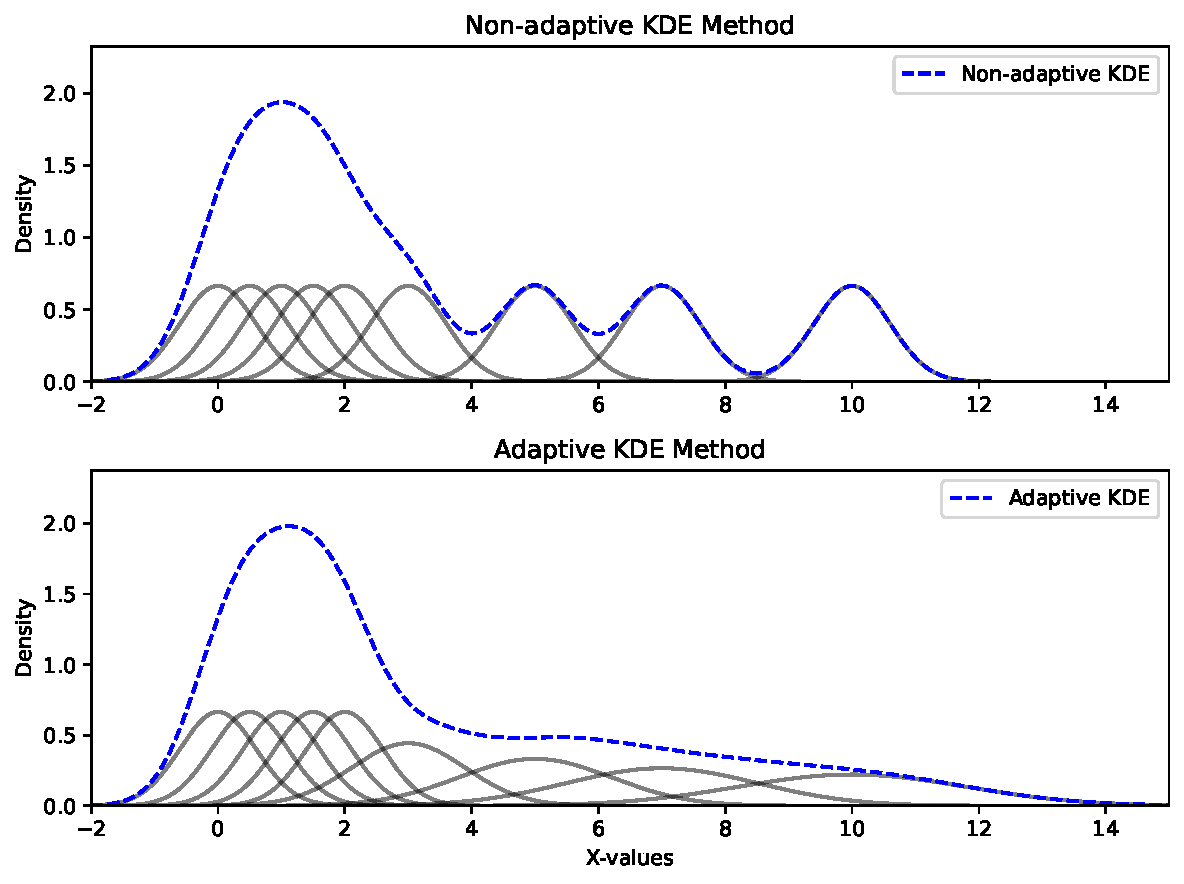
\includegraphics[width=0.6\linewidth]{4_photonid/ffs/smoothing/kde}
    \caption{Esquema del suavizado no adaptativo y adaptativo del método \ac{KDE}.}
    \label{fig:ss_corrections:ffs:calculation:adaptive_nonadaptive_kde}
\end{figure}

\begin{figure}[ht!]
    \centering
    \begin{subfigure}[h]{0.49\linewidth}
        \centering
        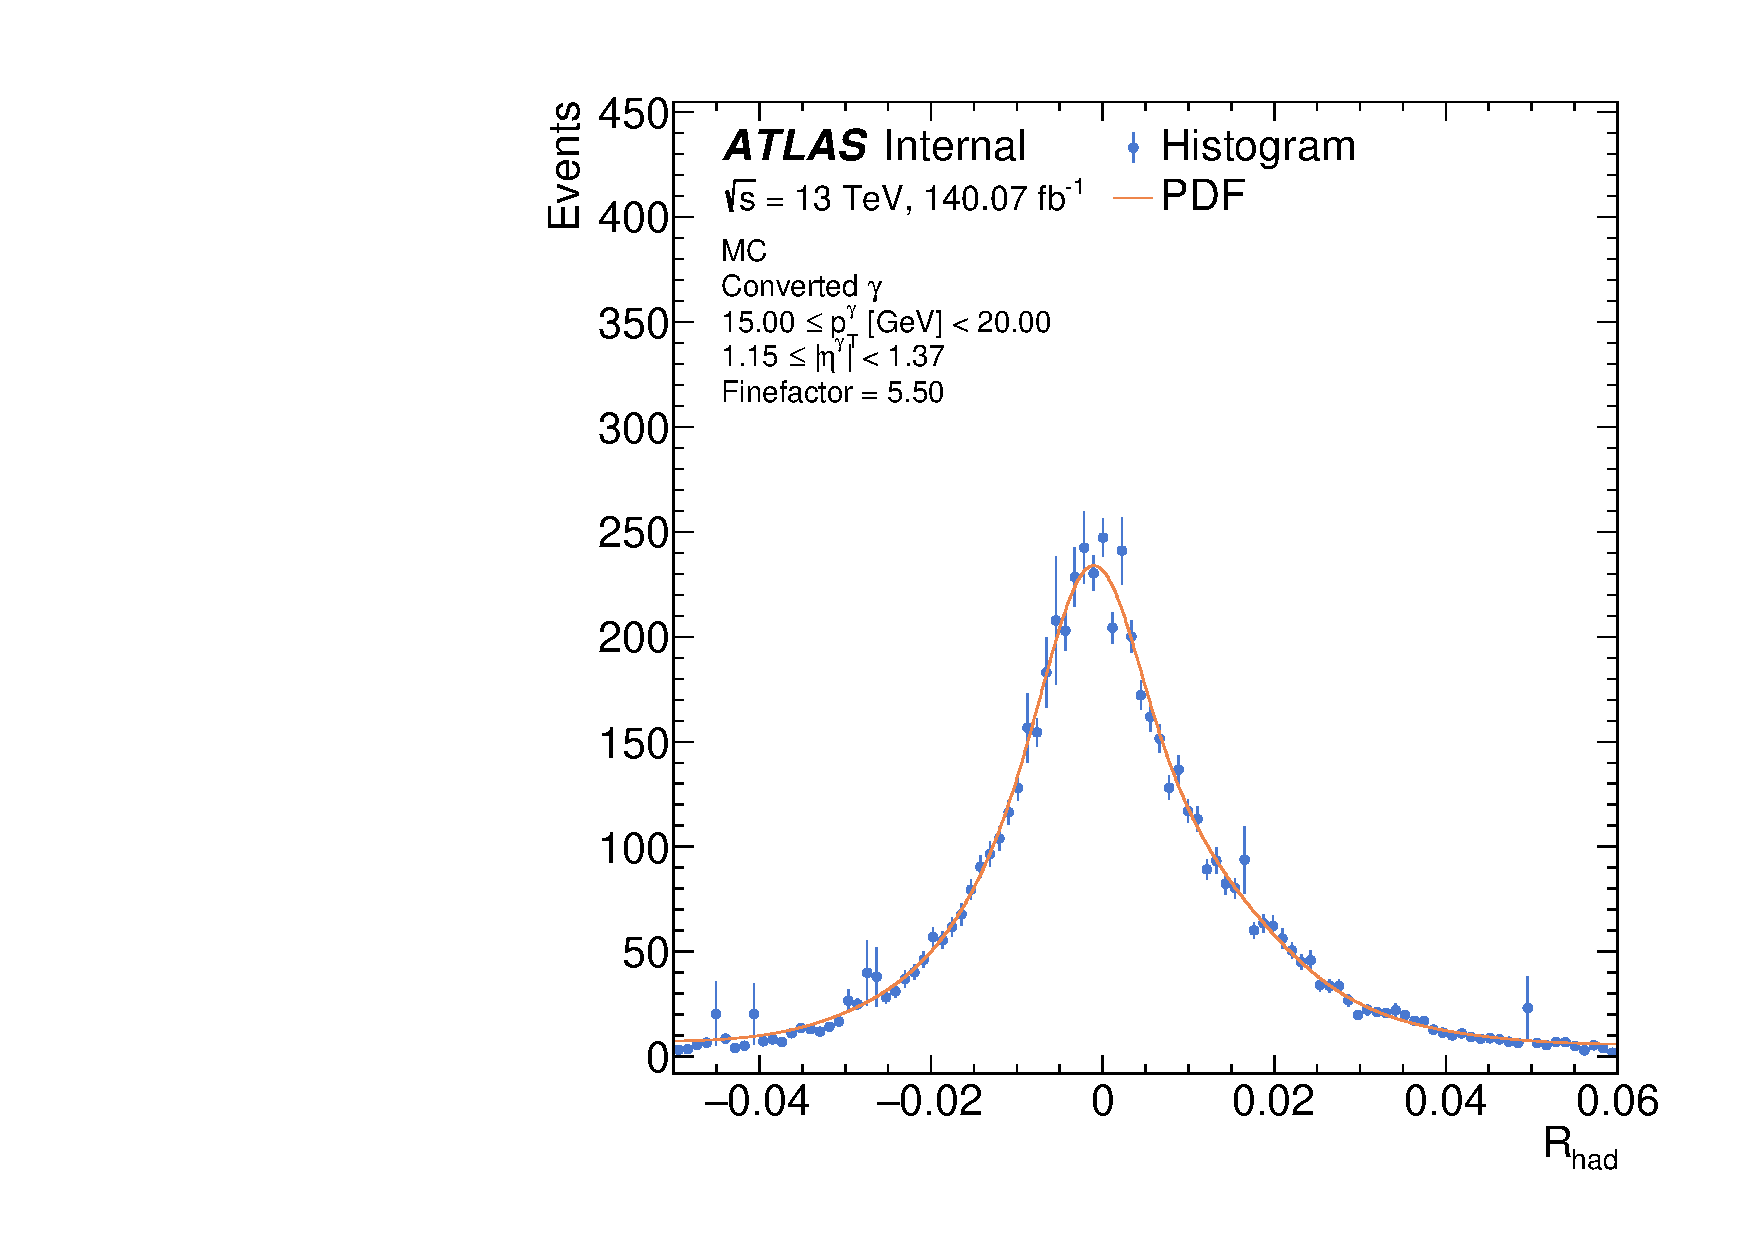
\includegraphics[width=\linewidth]{4_photonid/ffs/smoothing/can__pdfhist__mc__ph_rhad1__c_pt15p0_eta1p15}
        \caption{Caso de baja estadística: muestras de \ac{RZ}}
    \end{subfigure}
    \hfill
    \begin{subfigure}[h]{0.49\linewidth}
        \centering
        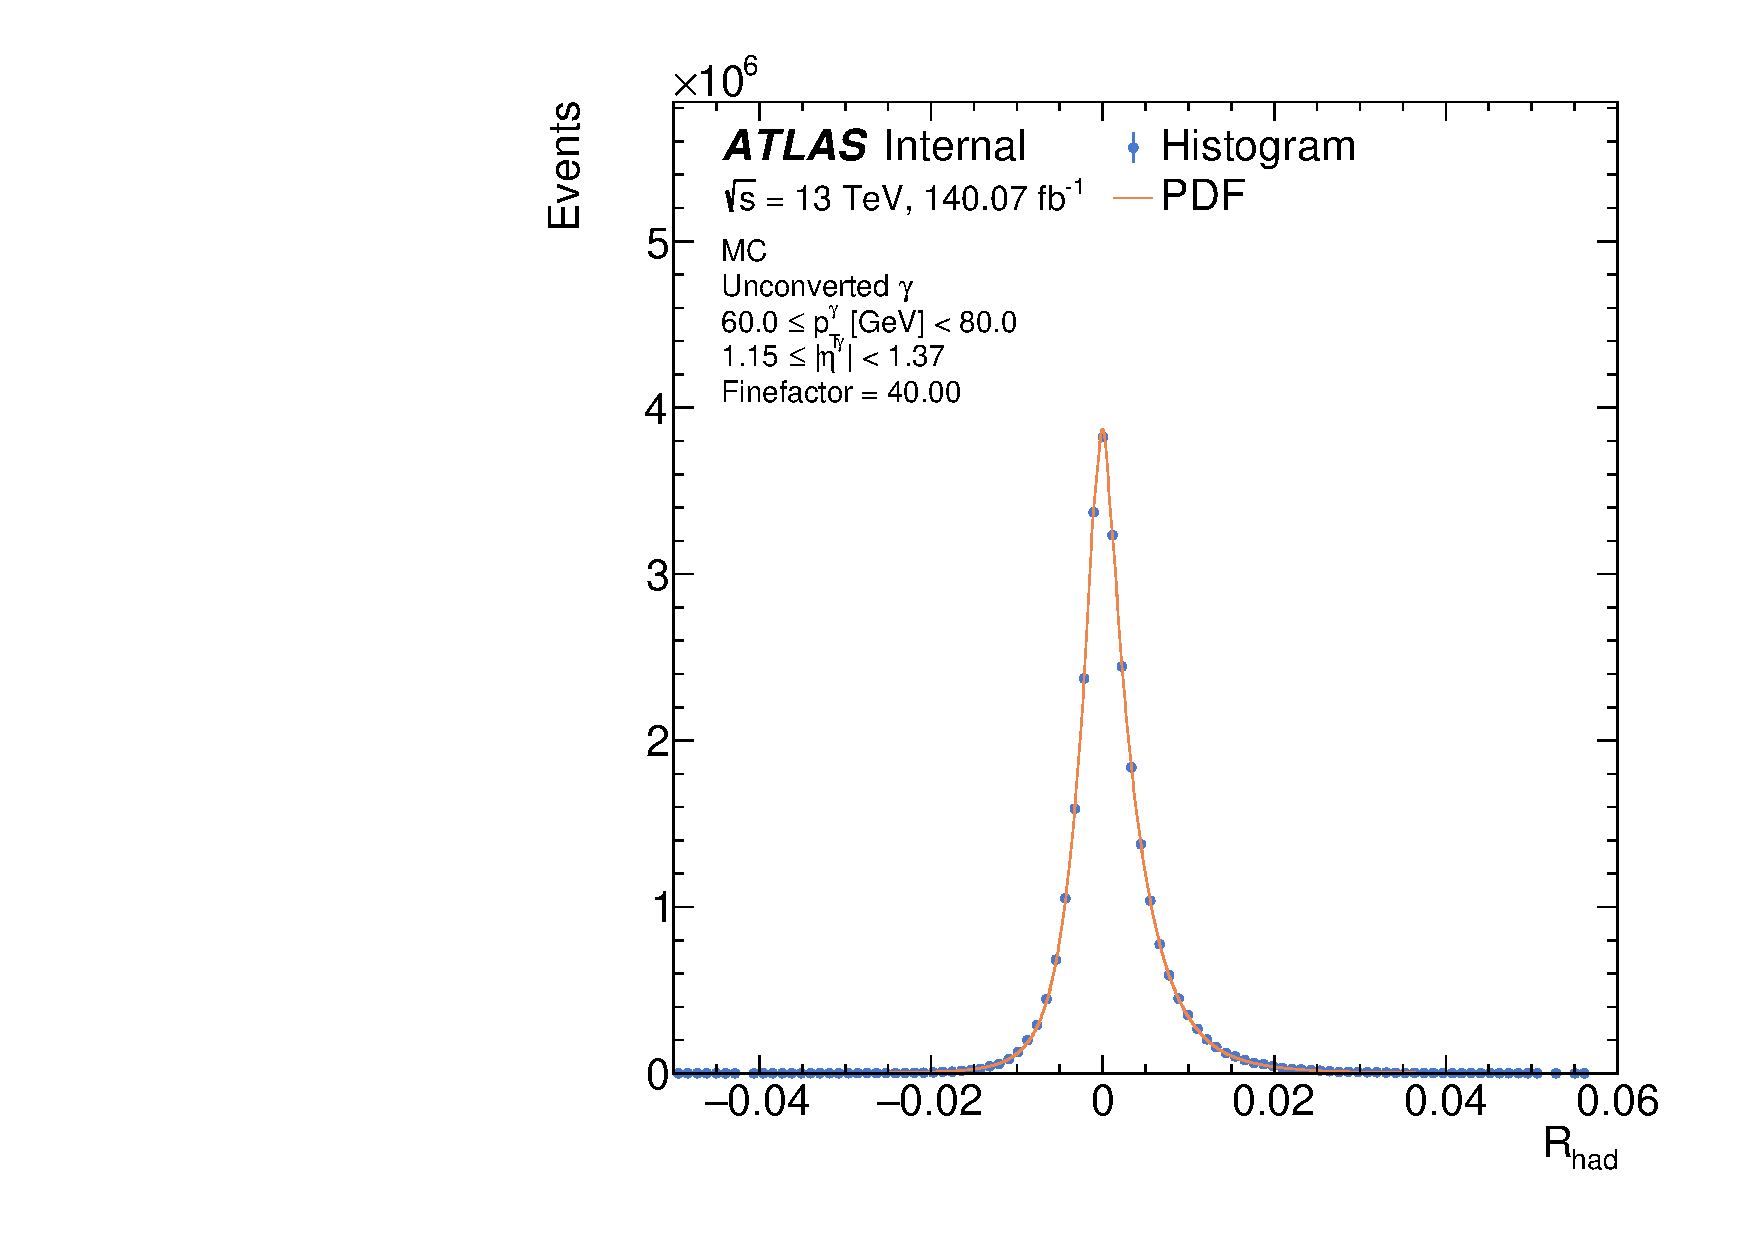
\includegraphics[width=\linewidth]{4_photonid/ffs/smoothing/can__pdfhist__mc__ph_rhad1__u_pt0060p0_eta1p15}
        \caption{Caso de alta estadística: muestras de \ac{SP}}
    \end{subfigure}
    \caption{Suavizado de la \ac{SS} \rhad utilizando el método \ac{KDE} para fotones en \(1.15<\abseta<1.37\) bajo dos posibles escenarios: baja y alta estadística. El histograma original se muestra con los puntos azules y las correspondientes \acp{PDF2} con la línea naranja. Además, se muestran los valores de los fine factors usados en cada caso.}
    \label{fig:ss_corrections:ffs:calculation:smoothing_ss}
\end{figure}


Una vez creadas las \acp{PDF2} de los datos y la simulación \ac{MC} para una dada variable, bin de \pt y \abseta y tipo de conversión, la \ac{PDF2} de \ac{MC} se normaliza a la de los datos y se calcula un valor \chisq entre ambos como~\cite{Chi2Histograms}:
\begin{equation}
	\chisq = \sum_{i=1}^{N} \dfrac{(w_{\text{MC},i} W_{\text{data}} - w_{\text{data},i} W_{\text{MC}})^2}{s_{\text{MC},i}^2 W_{\text{data}}^2 + s_{\text{data},i}^2 W_{\text{MC}}^2}.
\end{equation}
\(N\) es el número de bines de las \acp{PDF2}, \(w_{\text{MC},i}\) y \(w_{\text{data},i}\) son los números de eventos de \ac{MC} y datos en cada bin, respectivamente, \(s_{\text{MC},i}\) y \(s_{\text{data},i}\) son los errores del bin y, por último, \(W_{\text{data}}\) y \(W_{\text{MC}}\) son la suma de los pesos en datos y \ac{MC}, respectivamente.

\subsubsection{Correcciones \textit{shift-only}}

Las correcciones a las \acp{SS} de \ac{MC} han sido realizadas hasta el presente a partir de simples corrimientos de ellas. Estos corrimientos o desplazamientos se denominan, de aquí en adelante, \textit{shift fugde-factors} \ac{FF}, o simplemente \textit{shifts}.
Para ello, se desplaza a la \ac{PDF2} de \ac{MC} a la izquierda y a la derecha un bin a la vez.
El número inicial de bines que se debe desplazar a la distribución \ac{MC} se calcula mediante la diferencia de los valores medios de las distribuciones de datos y \ac{MC}. A partir de este valor inicial se consideran shifts de hasta 100 bines a cada lado.
Como consecuencia de este procedimiento la resolución del shift depende directamente del ancho del bin de la \ac{PDF2}, por lo que bines más pequeños conducen a una mejor resolución del shift. Dado que los histogramas, en primer lugar, se construyen con bines relativamente anchos, la \ac{PDF2} puede construirse utilizando bines pequeños de alta precisión para asegurar una alta resolución. Después de pruebas de convergencia de los \acp{FF}, se decide construir las \acp{PDF2} con 5000 bines.

Para cada bin que se ha desplazado la distribución se calcula y se registra el valor \chisq. Suponiendo que los errores \(s_{\text{MC},i}\) y \(s_{\text{data},i}\) tienen una distribución gaussiana estándar~\footnote{Este requsito se cumple siempre que los contenidos de los bines de ambas \acp{PDF2} sean mayores que 10, lo que también se satisface puesto que los histogramas se construyen con bines relativamente amplios.}, se espera que la forma seguida por los valores \chisq cerca del mínimo sea aproximadamente parabólica.

Para extraer los \acp{FF} se realiza un ajuste a los valores de \chisq cercanos al mínimo (5 bines a cada lado del bin mínimo) utilizando una función parabólica y el \ac{FF} de shift se obtiene a partir del mínimo ajustado. Por último, utlilizando este valor se puede corregir a la \ac{SS} evento a evento como:
\[
	x = x_{\text{old}} + \text{shift}.
\]
donde \(x_{\text{old}}\) y \(x\) representan el valor original y el valor post-corrección de la variable que se quiere corregir, respectivamente.


\subsubsection{Correcciones \textit{shift+stretch}}

Se observó que incluso después de aplicar correcciones de shift a las \acp{SS} de \ac{MC}, continuaban existiendo diferencias en las formas de las mismas y, en algunos casos, éstas pueden ser bastante sustanciales. 
En el contexto de esta tesis se propuso continuar mejorando las distribuciones introduciendo una corrección de orden superior a las simulaciones \ac{MC}, denominada \textit{stretching}. Las dos correcciones, actuando en conjunto, son denominadas como correcciones shift+stretch (o desplazamiento+estiramiento), que pretenden corregir simultáneamente el valor medio y los anchos de las distribuciones de \ac{MC}, presentadas en la \Refn{\cite{ATLAS-QT-Sili}}.

El método de corrección shift+stretch empieza por encontrar el máximo de la \ac{PDF2} de \ac{MC}. Posteriormente, la \ac{PDF2} se estira alrededor del máximo calculando la nueva posición de cada bin por el producto \(\text{stretch}\times (x - \text{stretch point})\), donde \(x\) es el centro del bin en cuestión. De este modo, el centro de cada bin conserva la distancia inicial al centro de la distribución, multiplicada por el factor de stretch. En el escenario en el que el stretch es \(>1\), puede haber casos en los que sea lo suficientemente grande como para dar lugar a bines vacíos. El contenido de estos bines vacíos se interpola linealmente a partir de los bines vecinos distintos de cero.
Una vez \textit{estirada} la \ac{PDF2}, se desplaza a izquierda y derecha siguiendo el mismo procedimiento que para el caso de shift-only, calculando los valores \chisq para cada \(\text{shift}_i\) después de aplicar el \(\text{stretch}_j\). Como resultado de este procedimiento, ahora se obtiene una grilla bidimensional de valores de \chisq en el plano de shift-stretch. El par shift-stretch se obtiene del centro del bin mínimo y comprende ahora los \acp{FF}. Las correcciones pueden ser aplicadas a cada \ac{SS} \(x\), evento a evento, como:
\begin{equation}
	x = \text{stretch}\times(x_{\text{old}} - \text{stretch point}) + \text{shift} + \text{stretch point},
\end{equation}
donde nuevamente \(x_\text{old}\) representa el valor de la variable sin corregir.

Un ejemplo de los valores de \chisq resultantes para la variable \fside se muestra en la \Fig{\ref{fig:ss_corrections:ffs:calculation:fside_calculation:chi2}}, donde el shift está representado en el eje \(x\) y el stretch en el eje \(y\). El valor óptimo de shift-stretch en este caso corresponde a \(\text{shift}=0.03\) y \(\text{stretch}=1.09\). En la \Fig{\ref{fig:ss_corrections:ffs:calculation:fside_calculation:pdfs}} se muestran las \acp{PDF2} antes y después de aplicar las correcciones donde se comparan con la \ac{PDF2} de los datos. Como se ve en la figura, hay una gran mejora y las distribuciones coinciden casi a la perfección.

\begin{figure}[ht!]
    \centering
    \begin{subfigure}[t]{0.49\linewidth}
        \centering
        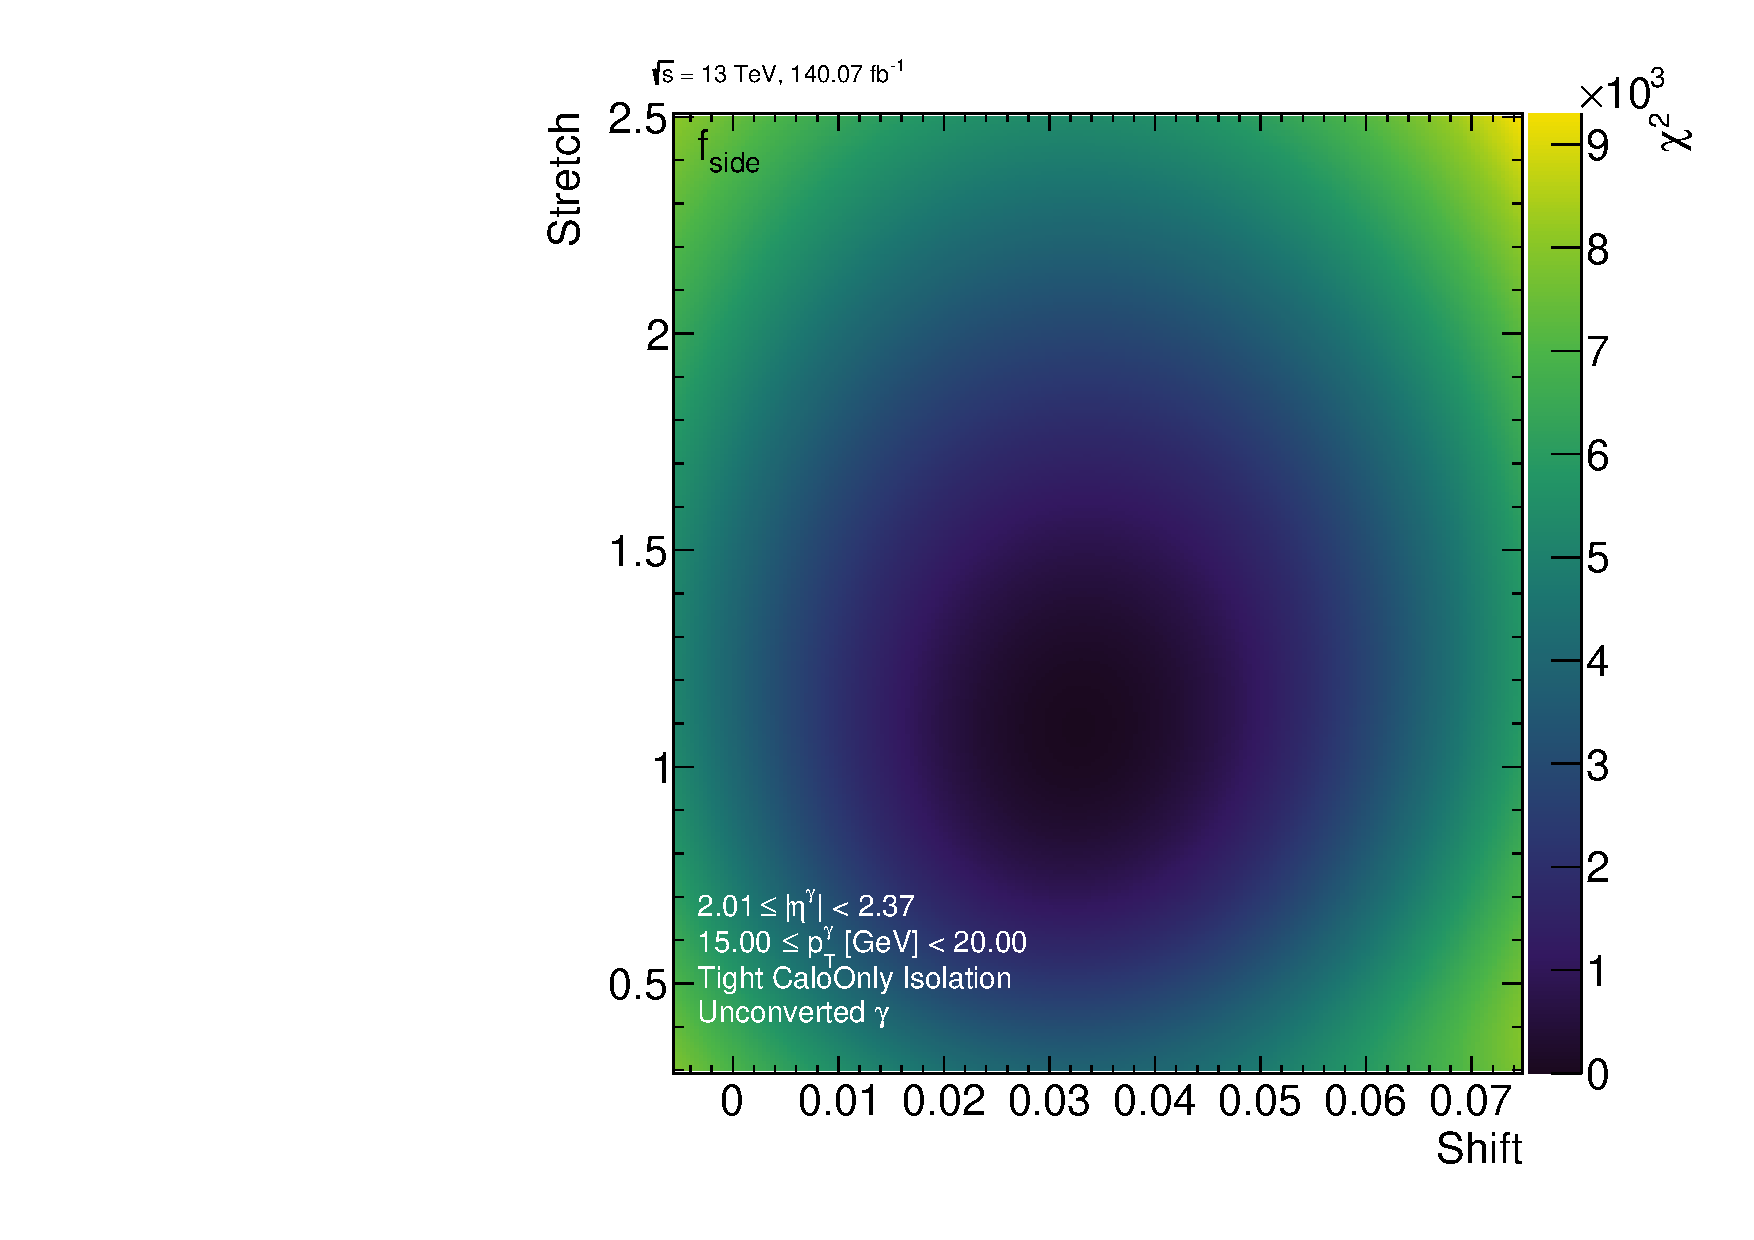
\includegraphics[width=\linewidth]{4_photonid/ffs/procedure/can2d__chi2scan_nocontour__ph_fside__Isotightcaloonly_IdNone_u_pt15p0_eta2p01}
        \caption{Valores de \chisq en el plano shift-stretch.}
        \label{fig:ss_corrections:ffs:calculation:fside_calculation:chi2}
    \end{subfigure}
    \hfill
    \begin{subfigure}[t]{0.49\linewidth}
        \centering
        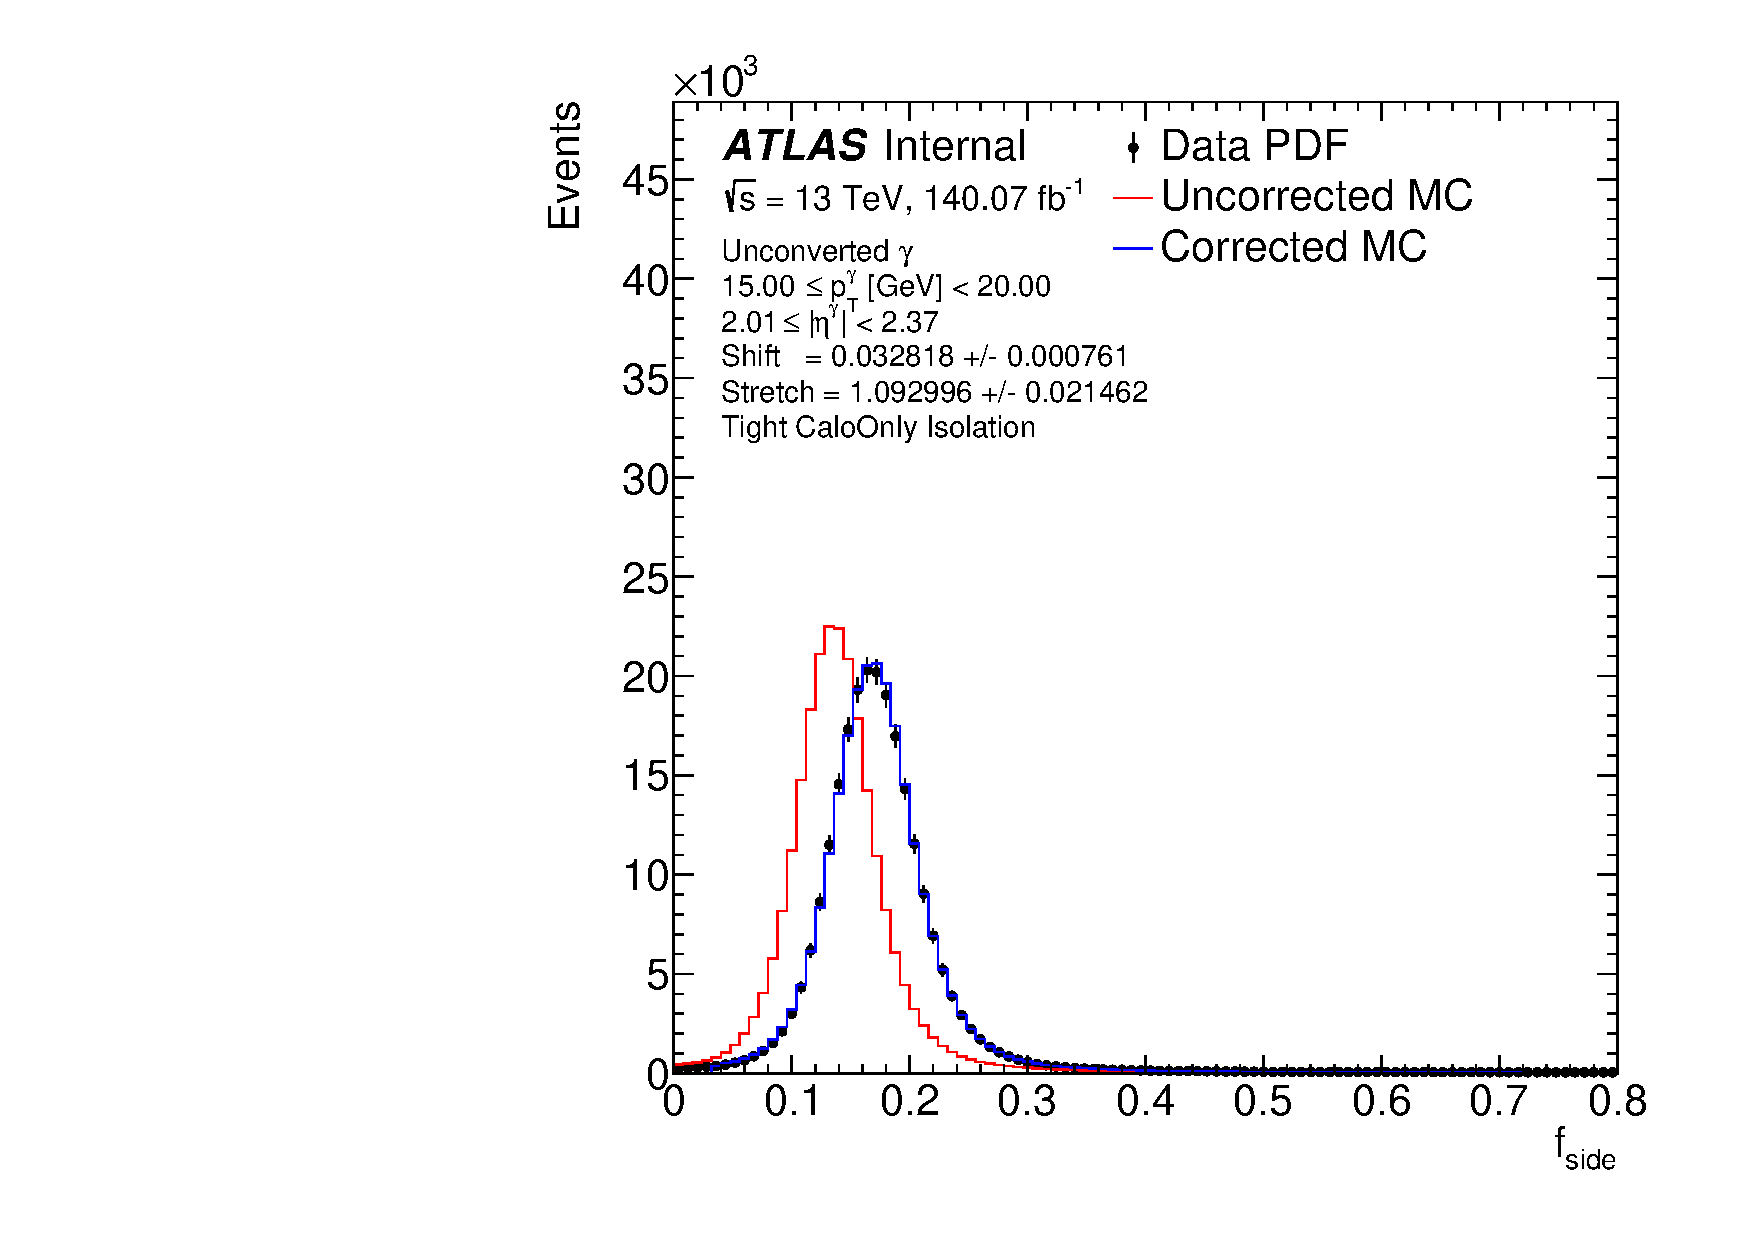
\includegraphics[width=\linewidth]{4_photonid/ffs/procedure/can__data_mc_fudged_comp__ph_fside__Isotightcaloonly_IdNone_u_pt15p0_eta2p01}
        \caption{\acp{PDF2} de datos (puntos negros) y simulación \ac{MC} sin corregir (línea roja) y corregida (línea azul), mostrando el impacto de las correcciones.}
        \label{fig:ss_corrections:ffs:calculation:fside_calculation:pdfs}
    \end{subfigure}
    \caption{Cálculo de los \acp{FF} de shift+stretch para \fside utilizando fotones no convertidos con momento transverso de \(15<\pt<20~\gev\) y pseudorapidez \(2.01<\abseta<2.37\) }
    \label{fig:ss_corrections:ffs:calculation:fside_calculation}
\end{figure}







\subsection{Cálculo de incertezas}
\label{subsec:ss_corrections:ffs:uncs}

\subsubsection{Incertezas estadísticas}

Para extraer las incertezas estadísticas de los \acp{FF} de shift y stretch, se realiza un ajuste al contorno de \(1\sigma\) (nivel de confianza del \(68.3\%\)) sobre los valores \chisq. Este contorno representa una elipse que toma la siguiente forma:
\begin{equation}
    \chi^2 = \chi^2_{\text{min}} + \frac{1}{1-\rho^2} \left[ \left( \frac{x-x_0}{\sigma_x} \right)^2 + \left( \frac{y-y_0}{\sigma_y} \right)^2 - 2\rho \left( \frac{x-x_0}{\sigma_x} \right) \left( \frac{y-y_0}{\sigma_y} \right) \right],
\end{equation}
donde \(\rho\) es el coeficiente de correlación entre ambas variables, \(\sigma_x\) y \(\sigma_y\) las incertezas sobre \(x\) y \(y\), respectivamente, \((x_0, y_0)\) es la posición del centro de la elipse y \(\chi^2_{\text{min}}\) es el valor mínimo de \(\chi^2\) obtenido del histograma bidimensional.


Extrayendo los semiejes mayor y menor de la elipse ajustada y con el ángulo de inclinación de la misma, las incertezas estadísticas sobre dos variables \(x\) y \(y\) (que en este caso representan el shift y el stretch, respectivamente) son (véase el \App{\ref{app:ellipse_formulae}}):
\begin{gather}
    \sigma_x = \sqrt{a^2 \cos^2\theta + b^2 \sin^2\theta}\\
    \sigma_y = \sqrt{a^2 \sin^2\theta + b^2 \cos^2\theta}.
\end{gather}

\subsubsection{Incertezas sistemáticas}

Las incertezas sistemáticas se obtienen variando los criterios de preselección, es decir, la identificación y el aislamiento de fotones. El cambio de los diferentes criterios de preselección permite que las \acp{SS} varíen dependiendo de la cantidad de contaminación de fondo, y en consecuencia también lo hacen los \acp{FF}.
Las diferentes selecciones son, para cada muestra:
\begin{itemize}
    \item \acf{RZ}:
        \begin{itemize}
            \item Nominal: Sin criterio de identificación, aislamiento \texttt{TightCaloOnly}.
            \item Identificación \texttt{Loose}, sin aislamiento.
            \item Identificación \texttt{Loose}, aislamiento \texttt{TightCaloOnly}.
            \item Sin identificación, aislamiento \texttt{Loose}.
        \end{itemize}
    \item \acf{SP}:
        \begin{itemize}
            \item Nominal: identificación \texttt{Tight}, aislamiento \texttt{Loose}.
            \item Identificación \texttt{Tight}, aislamiento \texttt{Tight} .
        \end{itemize}
\end{itemize}
Todas las demás combinaciones (o falta de ellas) de criterios de selección darían como resultado una muestra con estadísticas demasiado bajas o una muy baja pureza.

Los \acp{FF} se derivan para cada una de las selecciones anteriores calculando la diferencia entre la nominal y la variada. La diferencia máxima se toma como incerteza sistemática, como el caso más conservativo. Finalmente, las incertezas estadísticas y sistemáticas se suman en cuadratura.










\subsection{Resultados}
\label{subsec:ss_corrections:ffs:results}


Debido al hecho de que los \acp{FF} se calculan en un amplio rango de \pt y utilizando dos muestras distintas que abarcan regiones complementarias, los resultados se concatenan en \(50~\gev\) donde ocurre la superposición entre ambas.


En la \Fig{\ref{fig:ss_corrections:ffs:reslts:ffs}} se presentan ejemplos de los \acp{FF} resultantes para las variables \reta y \weta utilizando fotones convertidos.
Los valores de shift se normalizan utilizando la desviación estándar de la \ac{SS} luego de aplicar el \ac{FF} de stretch, ya que esta cantidad permite comprender cuánto se desplaza cada variable con respecto a su ancho. Además, proporciona una medida única para todas las variables consideradas ya que cada una de ellas abarca rangos diferentes. No obstante, el ancho de las variables varía según los distintos bines de \pt y \abseta lo que puede dar lugar a grandes diferencias entre bines vecinos.
Se puede observar que para ambas variables los \acp{FF} dependen de \pt, especialmente hacia momentos transversos más altos. Este comportamiento también se repite en todas las variables.
Inspeccionando los comportamientos y tendencias de los \acp{FF} también es posible recuperar información sobre el deficiente modelado de las \acp{SS} por el \ac{MC}. Como se mencionó en la \Sect{\ref{sec:pid_ss:ss_differences}}, se observaron anchos y perfiles en \(\eta\) más amplios para los datos en comparación con la simulación. De hecho, esto se puede inferir dado que los valores de stretch aumentan a valores más altos de \pt estirando las simulaciones \ac{MC} hasta el doble de su ancho inicial. En el caso de \reta (\weta) mostrado, la simulación \ac{MC} sobreestima (subestima) el valor central de la distribución en casi una desviación estándar después de corregir el ancho, lo que significa que las diferencias entre la distribución \ac{MC} sin corregir con la de los datos son muy grandes.

\begin{figure}[ht!]
    \centering
    \begin{subfigure}[h]{0.49\linewidth}
        \centering
        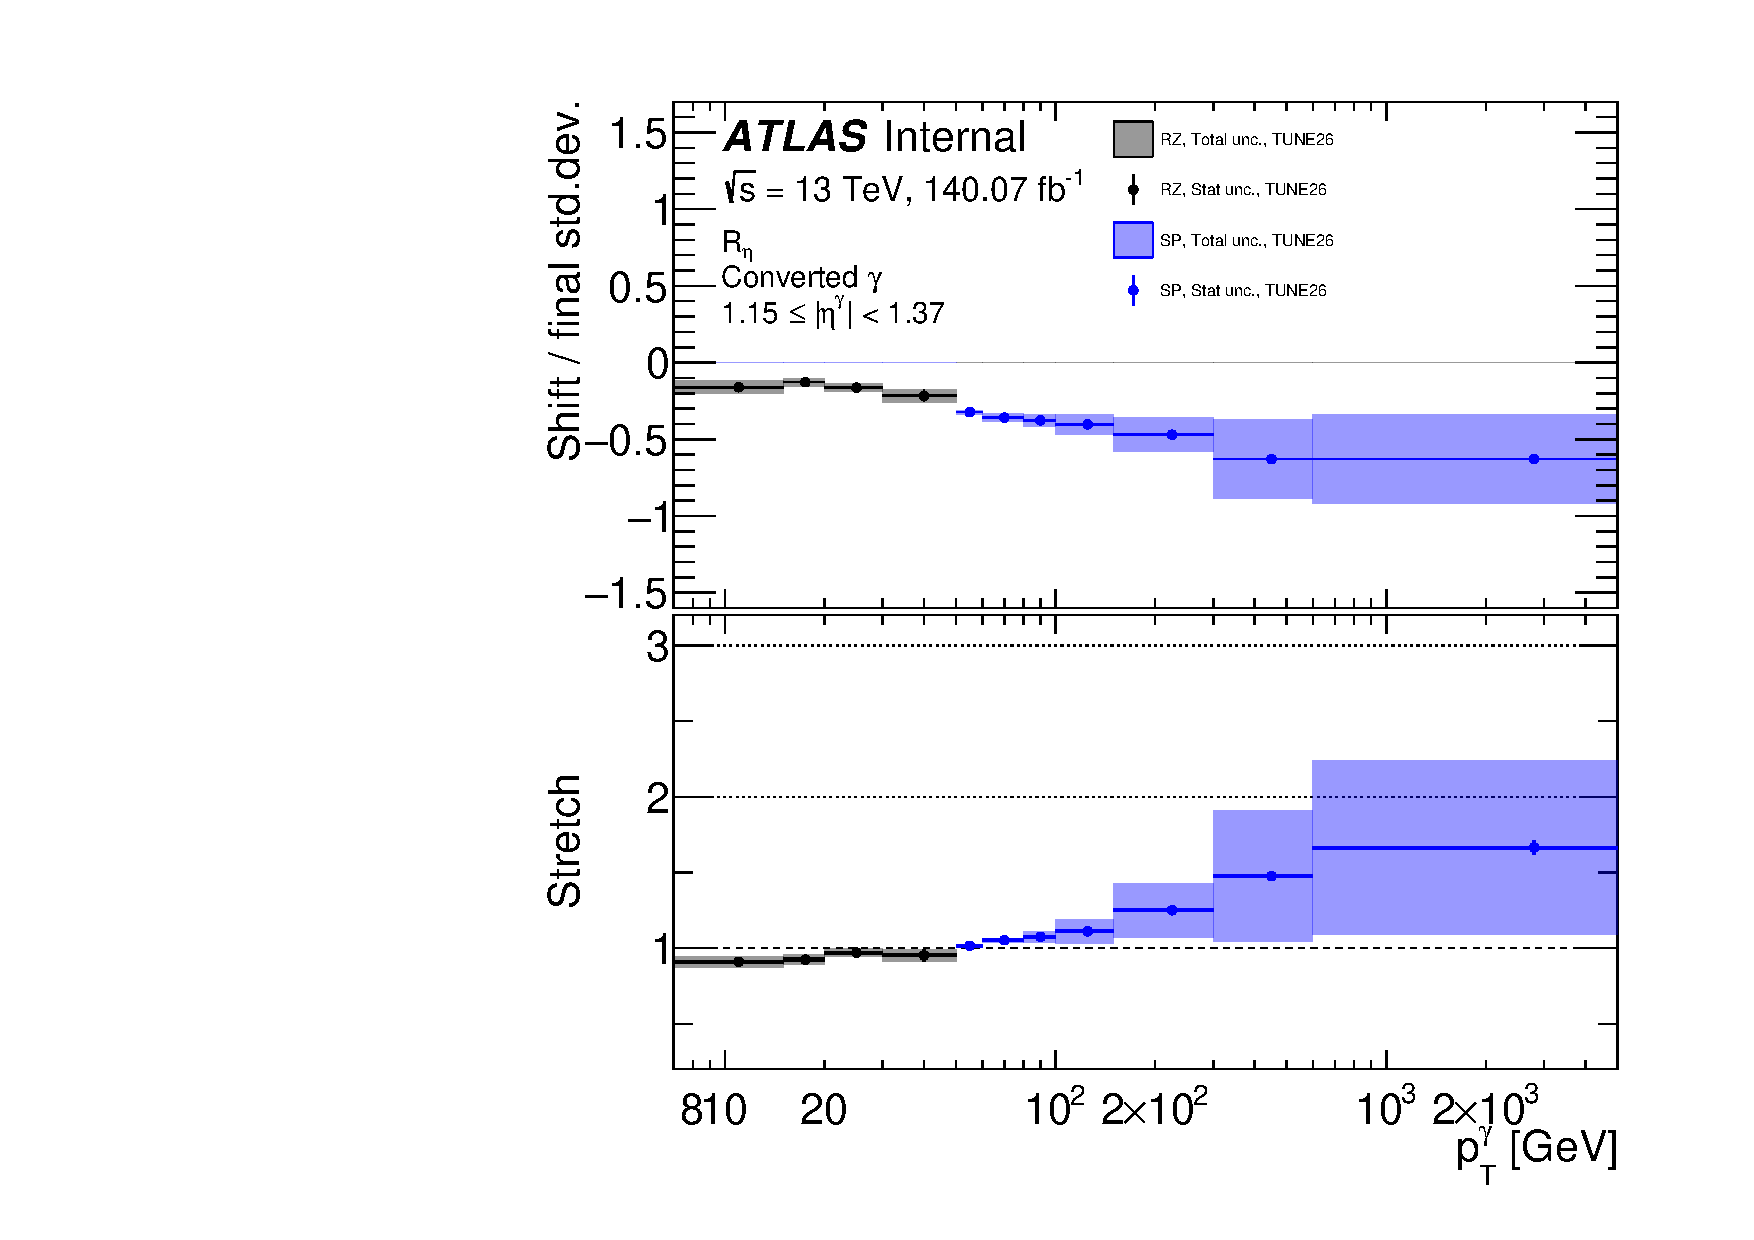
\includegraphics[width=\linewidth]{4_photonid/ffs/results/combined/1d/can__comb__ph_reta__c__eta1p15__shift_normalized}
        \caption{\reta}
        \label{fig:ss_corrections:ffs:reslts:ffs:reta}
    \end{subfigure}
    \hfill
    \begin{subfigure}[h]{0.49\linewidth}
        \centering
        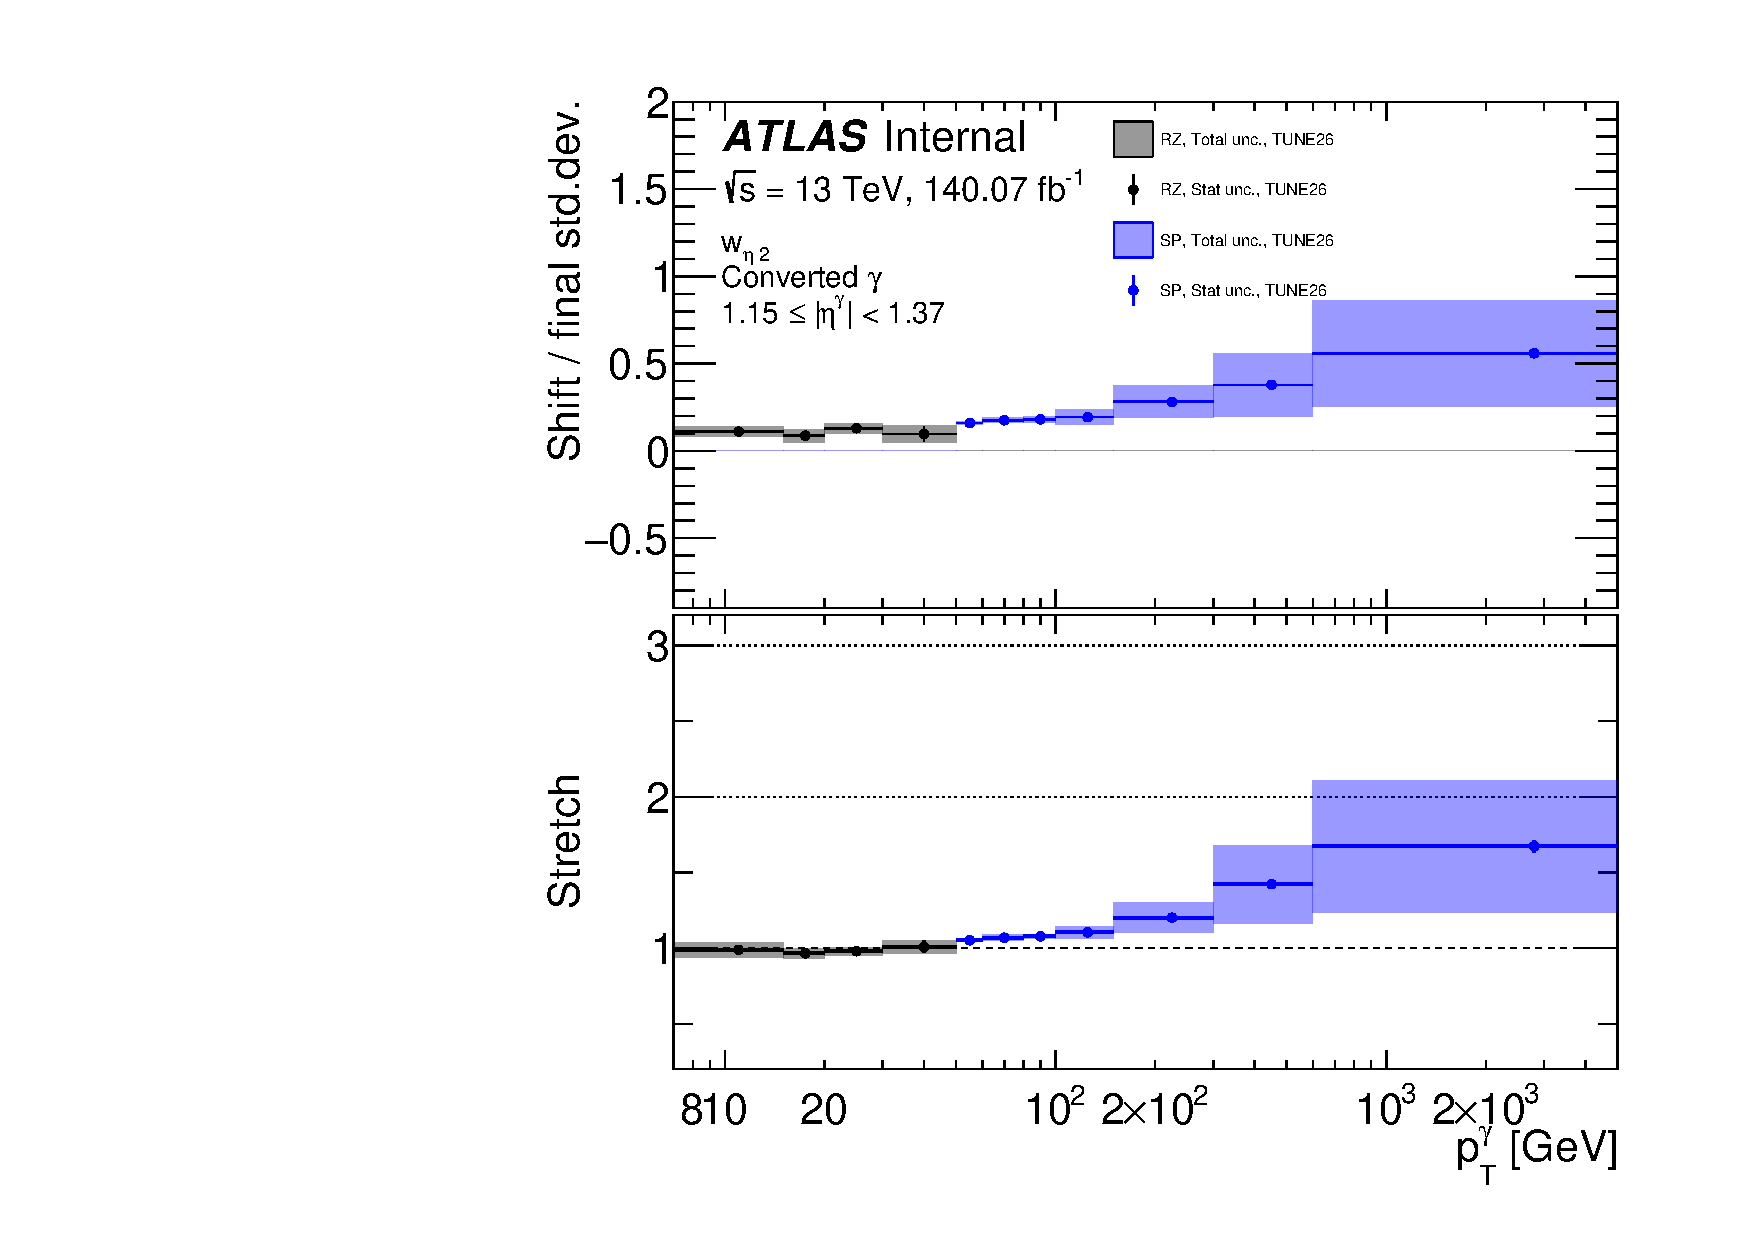
\includegraphics[width=\linewidth]{4_photonid/ffs/results/combined/1d/can__comb__ph_weta2__c__eta1p15__shift_normalized}
        \caption{\weta}
        \label{fig:ss_corrections:ffs:reslts:ffs:weta}
    \end{subfigure}
    \caption{Valores de los \acp{FF} de shift y stretch para las \reta (izquierda) y \weta (derecha) para fotones convertidos con \(1.15<\abseta<1.37\), en función de \pt. Los resultados obtenidos por las muestras de \ac{RZ} están representados por el color negro, mientras que los resultados de \ac{SP} se muestran en azul. Los puntos y las líneas denotan los valores centrales con sus incertezas estadísticas, mientras que las regiones sombreadas representan las incertezas totales. Los valores de shift se muestran en el panel superior, los cuales son normalizados por el ancho de la distribución luego de ser estirada por el stretch, como se ha explicado en el texto. Este último valor se muestra en el panel inferior de las figuras.}
    \label{fig:ss_corrections:ffs:reslts:ffs}
\end{figure}

También es útil visualizar los \acp{FF} en un bin de \pt fijo y en función de \abseta para así determinar qué tan dependientes de \abseta son las correcciones. Esto se muestra para \wstot utilizando fotones convertidos con \(50<\pt<60~\gev\) en la \Fig{\ref{fig:ss_corrections:ffs:reslts:ffs_eta_wstot}}. Como se puede notar, para \(\abseta>1.81\) (los dos últimos bines), los valores de shift normalizados son mayores que los de los bines anteriores en, al menos, un factor 2. Sin embargo, los valores de shift sin normalizar mostrados en la \Fig{\ref{fig:ss_corrections:ffs:reslts:ffs_eta_wstot:raw_shift}} no presentan un cambio tan marcado observándose sólo una pequeña dependencia en \abseta. Como consecuencia de este comportamiento se puede concluir que el cambio brusco observado es debido al cambio en el ancho de la distribución entre los distintos bines de \abseta, tal como se había anticipado.


\begin{figure}[ht!]
    \centering
    \begin{subfigure}[h]{0.49\linewidth}
        \centering
        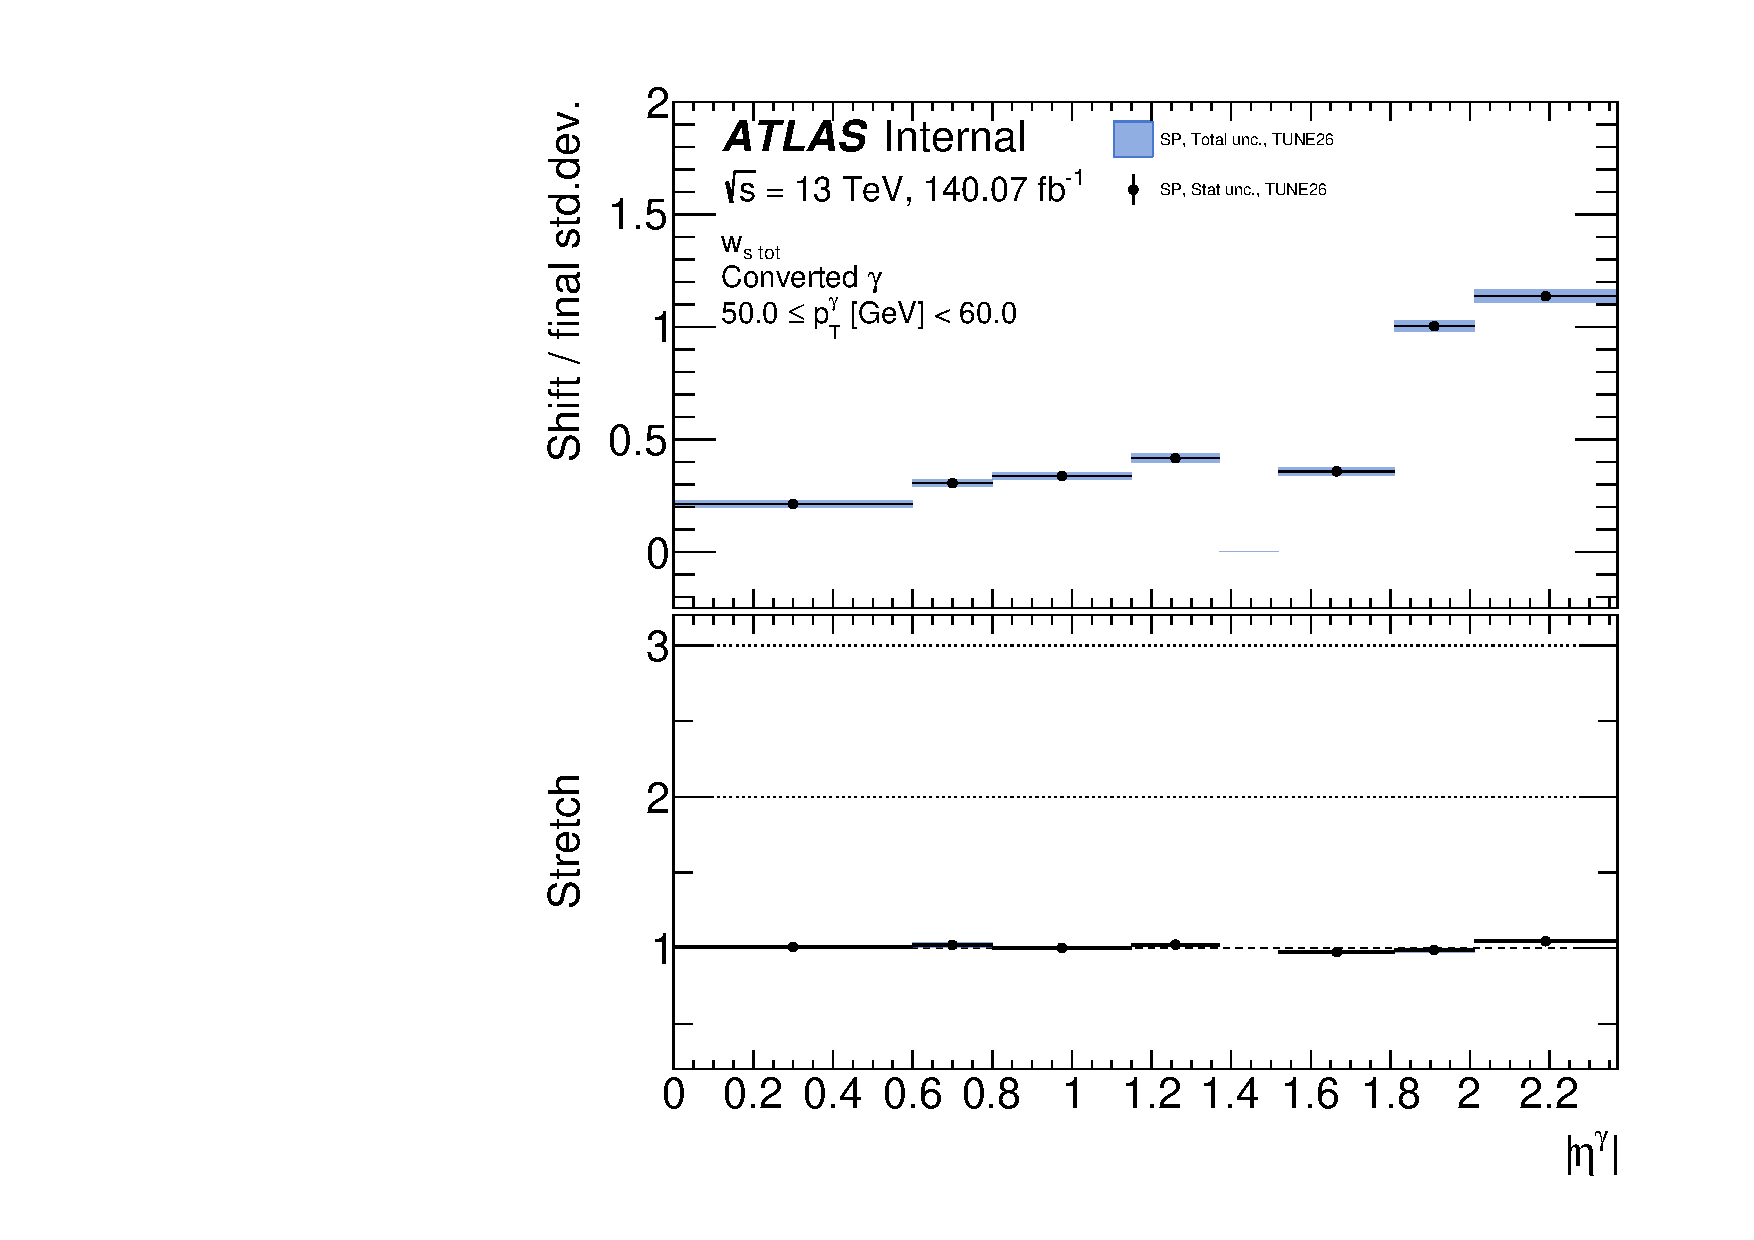
\includegraphics[width=\linewidth]{4_photonid/ffs/results/SP/1d/can__SP__ph_wstot__c__pt0050p0__shift_normalized}
        \caption{Valores de shift normalizados.}
        \label{fig:ss_corrections:ffs:reslts:ffs_eta_wstot:normalised_shift}
    \end{subfigure}
    \hfill
    \begin{subfigure}[h]{0.49\linewidth}
        \centering
        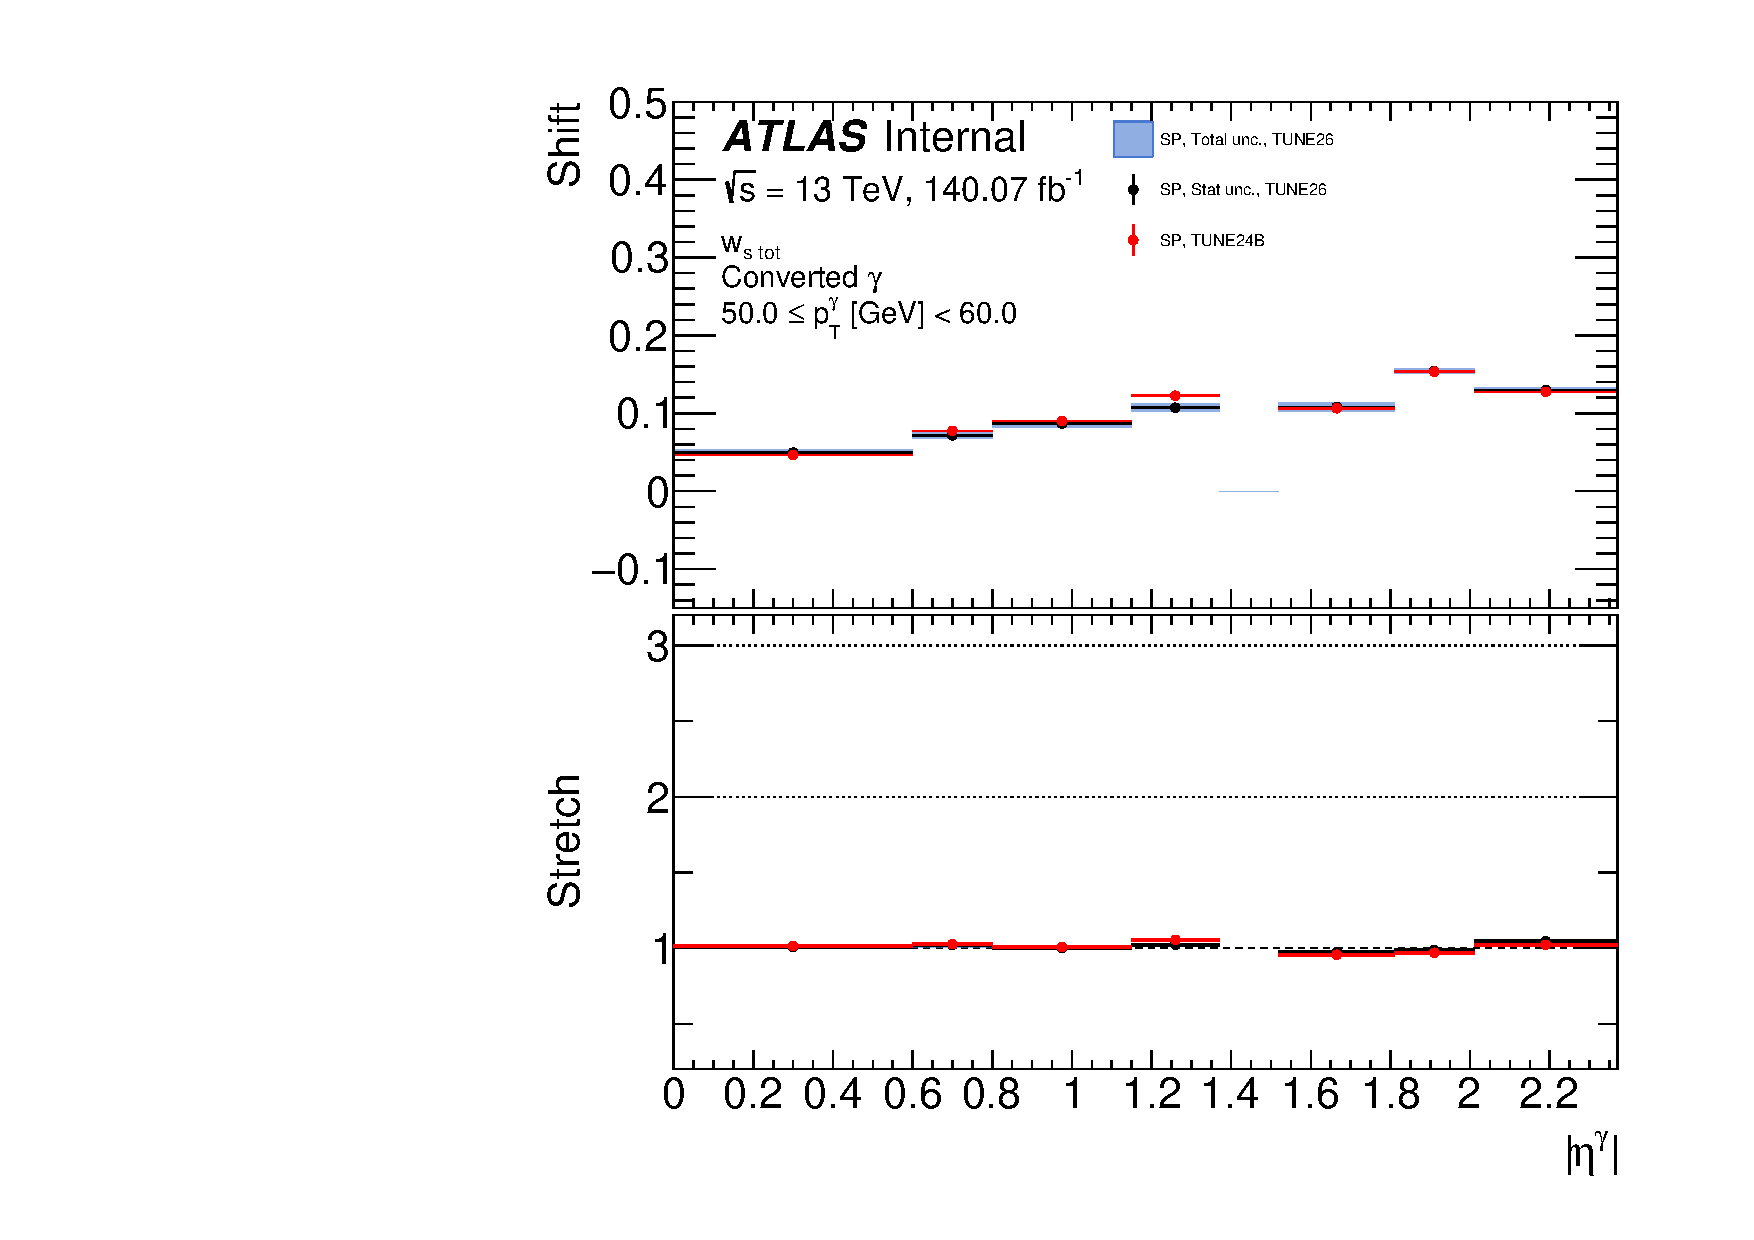
\includegraphics[width=\linewidth]{4_photonid/ffs/results/SP/1d/can__SP__ph_wstot__c__pt0050p0}
        \caption{Valores de shift sin normalizar.}
        \label{fig:ss_corrections:ffs:reslts:ffs_eta_wstot:raw_shift}
    \end{subfigure}\\
    \caption{Valores de los \acp{FF} de shift y stretch para \wstot en función de \abseta utilizando fotones convertidos con \(50<\pt<60~\gev\) de las muestras de \ac{SP}. La \Fig{\subref{fig:ss_corrections:ffs:reslts:ffs_eta_wstot:normalised_shift}} muestra los valores de shift normalizados, mientras que los no normalizados se encuentra en la \Fig{\subref{fig:ss_corrections:ffs:reslts:ffs_eta_wstot:raw_shift}}. Los puntos con las líneas de color muestran los valores centrales y las incertezas estadísticas, mientras que las áreas sombreadas representan las incertezas totales en cada bin. Los valores de stretch se muestran en los paneles inferiores de cada figura.}
    \label{fig:ss_corrections:ffs:reslts:ffs_eta_wstot}
\end{figure}


Para validar los \acp{FF} obtenidos las correcciones se aplican a las \acp{SS} evento por evento.
Las \Figs{\ref{fig:ss_corrections:ffs:results:ss_rz}}{\ref{fig:ss_corrections:ffs:results:ss_sp}} muestrans \acp{SS} luego de aplicar los \acp{FF} utilizando las muestras \ac{RZ} y \ac{SP}, respectivamente, divididas en las regiones barrel y endcap en \abseta. Las correcciones mejoran el acuerdo entre datos y \ac{MC} en la región barrel, pero la mejora no es tan significativa como en la región endcap, donde se observa un acuerdo excelente entre datos y \ac{MC}. Tomando como ejemplo las variables \wone y \wstot, se observan grandes diferencias en las formas entre la simulación nominal y los datos que los métodos shift+stretch consiguen corregir. El mismo comportamiento se observa con las muestras \ac{SP}, en las que estas variables presentan dos o más picos, y que se corrigen correctamente con el método de \acp{FF}. En todos los casos mostrados, el \ac{MC} corregido y los datos son casi indistinguibles lo que demuestra la importancia de estas correcciones y cómo logran un excelente acuerdo.

\begin{figure}[ht!]
    \centering
    \begin{subfigure}[h]{0.32\linewidth}
        \centering
        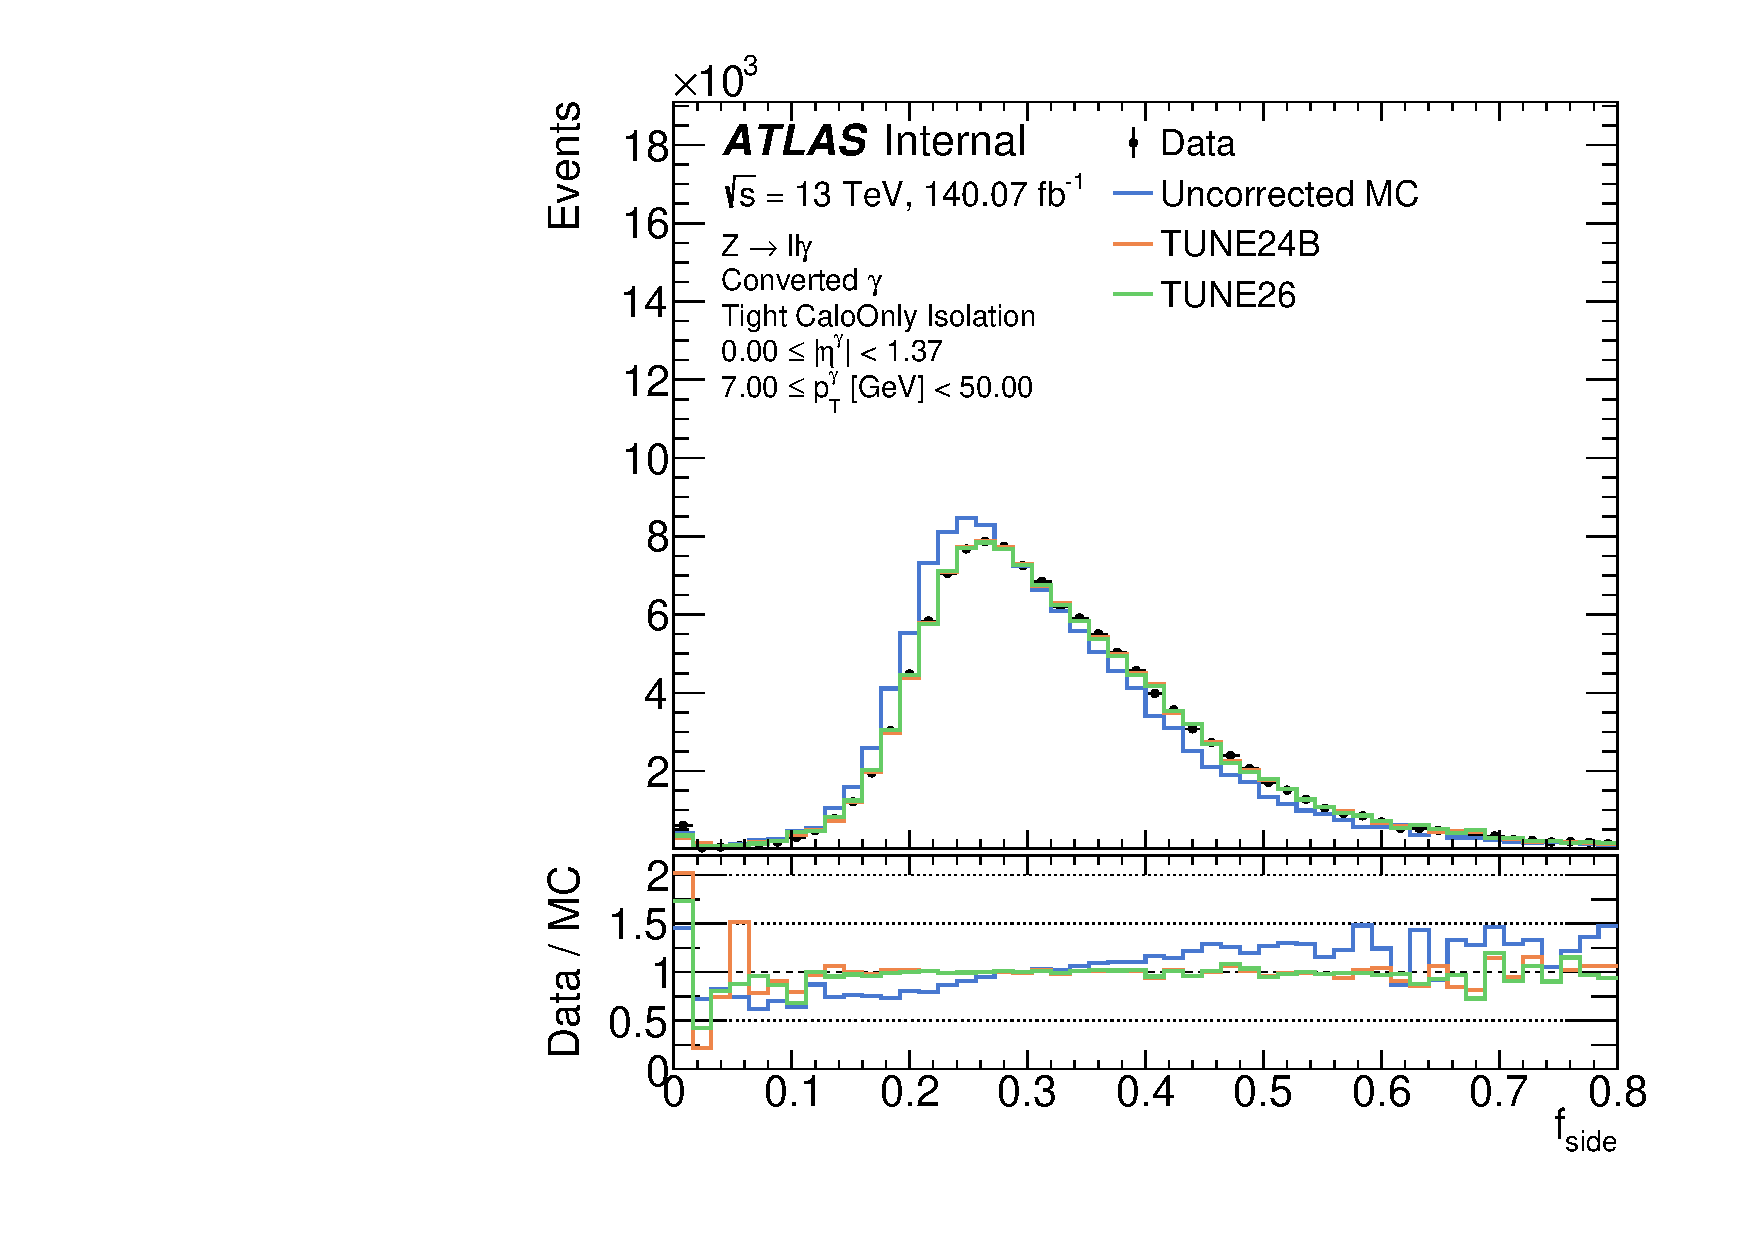
\includegraphics[width=\linewidth]{4_photonid/ffs/results/RZ/corrections/c/ptFull/etaCoarse/can__correction__ph_fside__Isotightcaloonly_IdNone__c__ptFullpt07p0__etaCoarseeta0p00}
        \caption{\fside, barrel.}
    \end{subfigure}
    \hfill
    \begin{subfigure}[h]{0.32\linewidth}
        \centering
        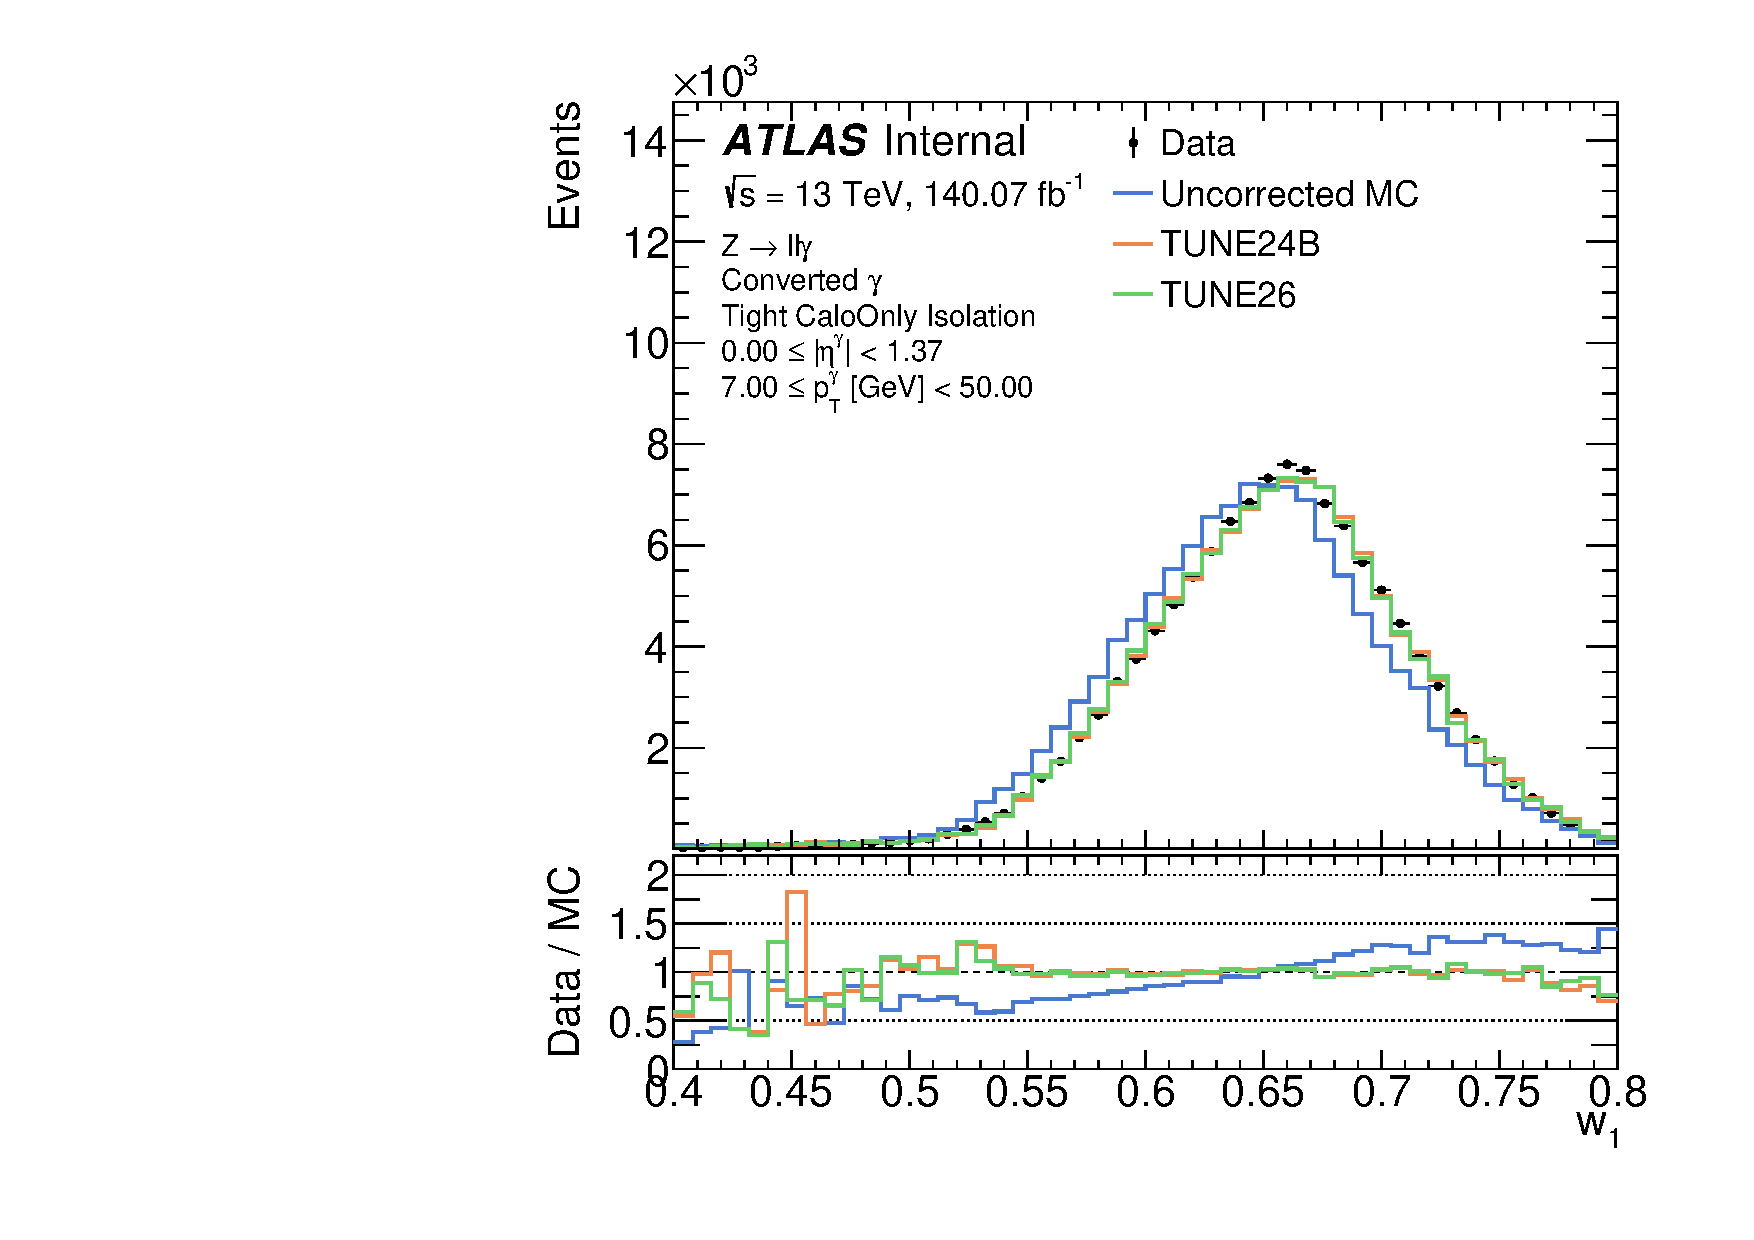
\includegraphics[width=\linewidth]{4_photonid/ffs/results/RZ/corrections/c/ptFull/etaCoarse/can__correction__ph_w1__Isotightcaloonly_IdNone__c__ptFullpt07p0__etaCoarseeta0p00}
        \caption{\wone, barrel.}
    \end{subfigure}
    \hfill
    \begin{subfigure}[h]{0.32\linewidth}
        \centering
        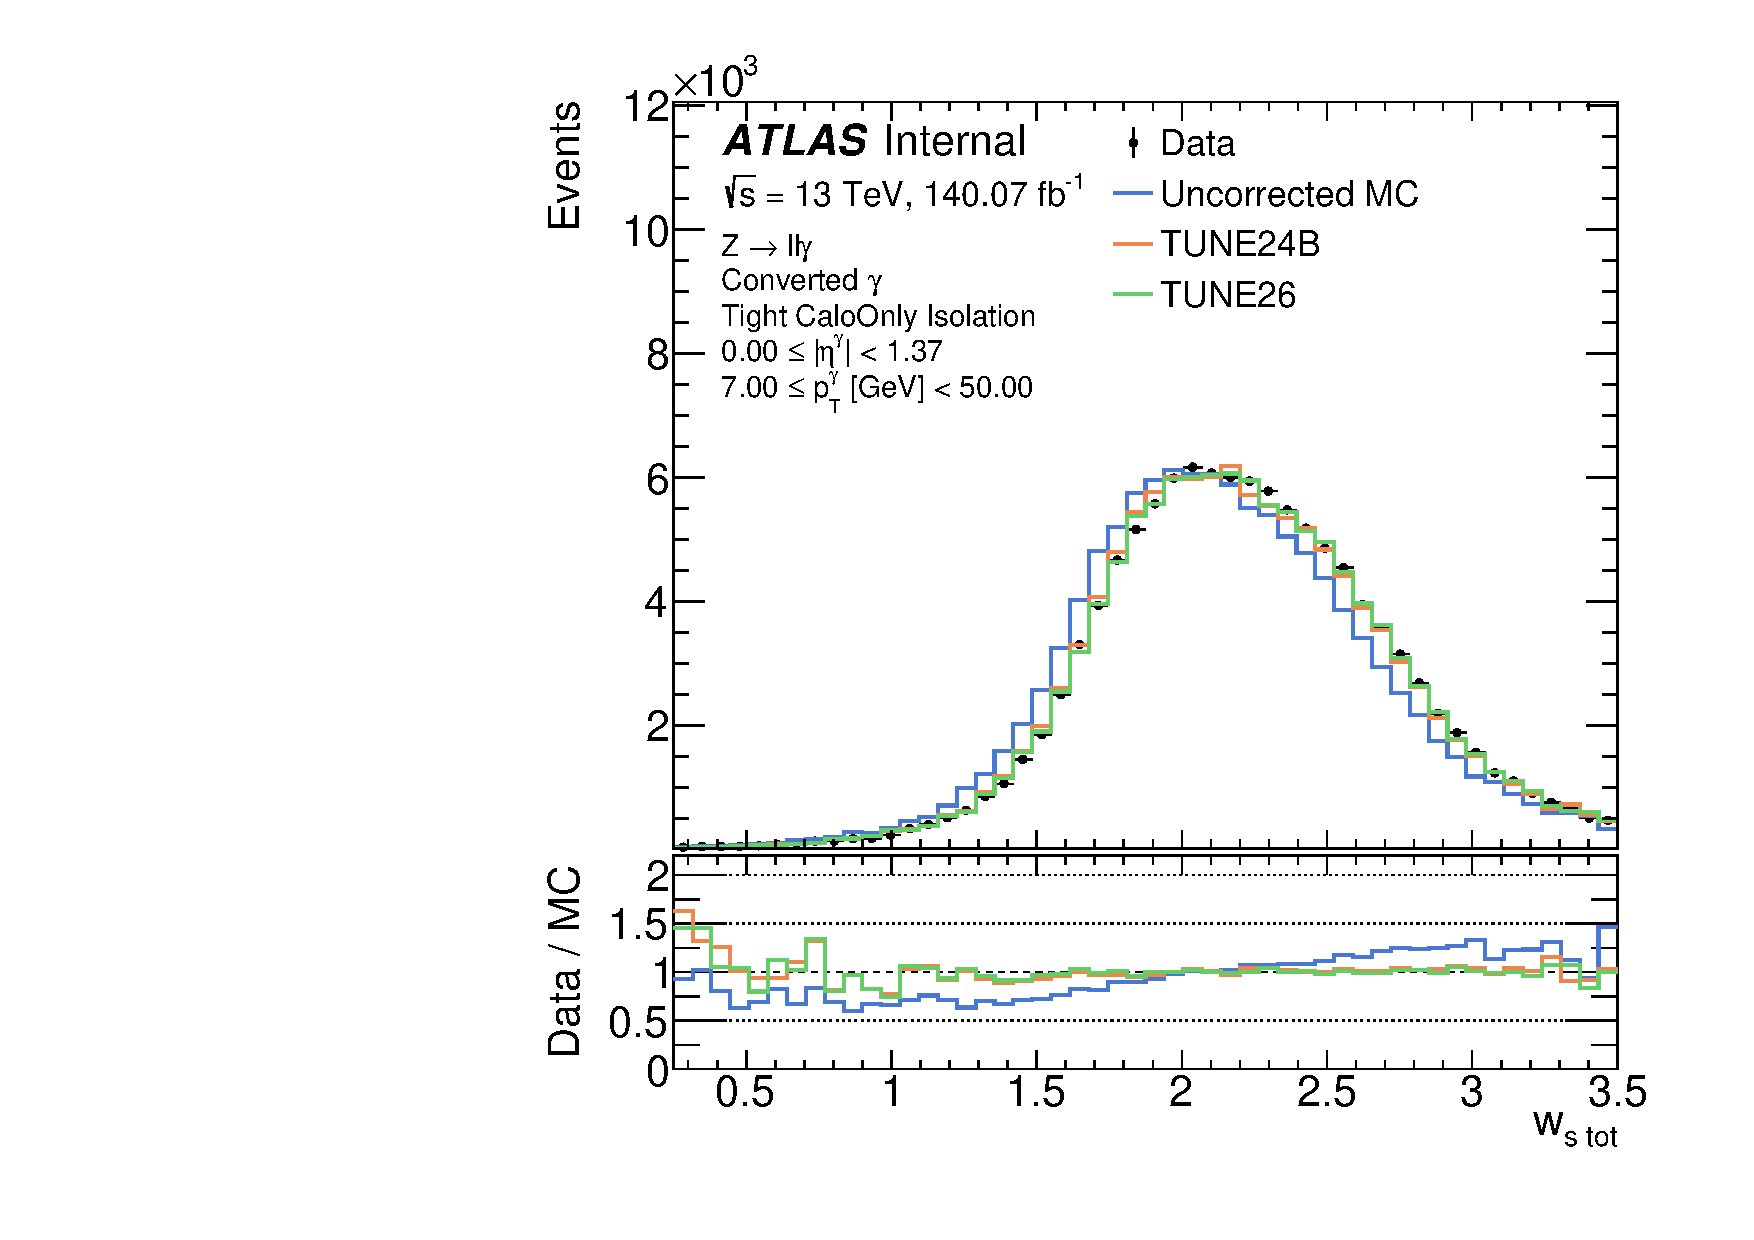
\includegraphics[width=\linewidth]{4_photonid/ffs/results/RZ/corrections/c/ptFull/etaCoarse/can__correction__ph_wstot__Isotightcaloonly_IdNone__c__ptFullpt07p0__etaCoarseeta0p00}
        \caption{\wstot, barrel.}
    \end{subfigure}\\
    \begin{subfigure}[h]{0.32\linewidth}
        \centering
        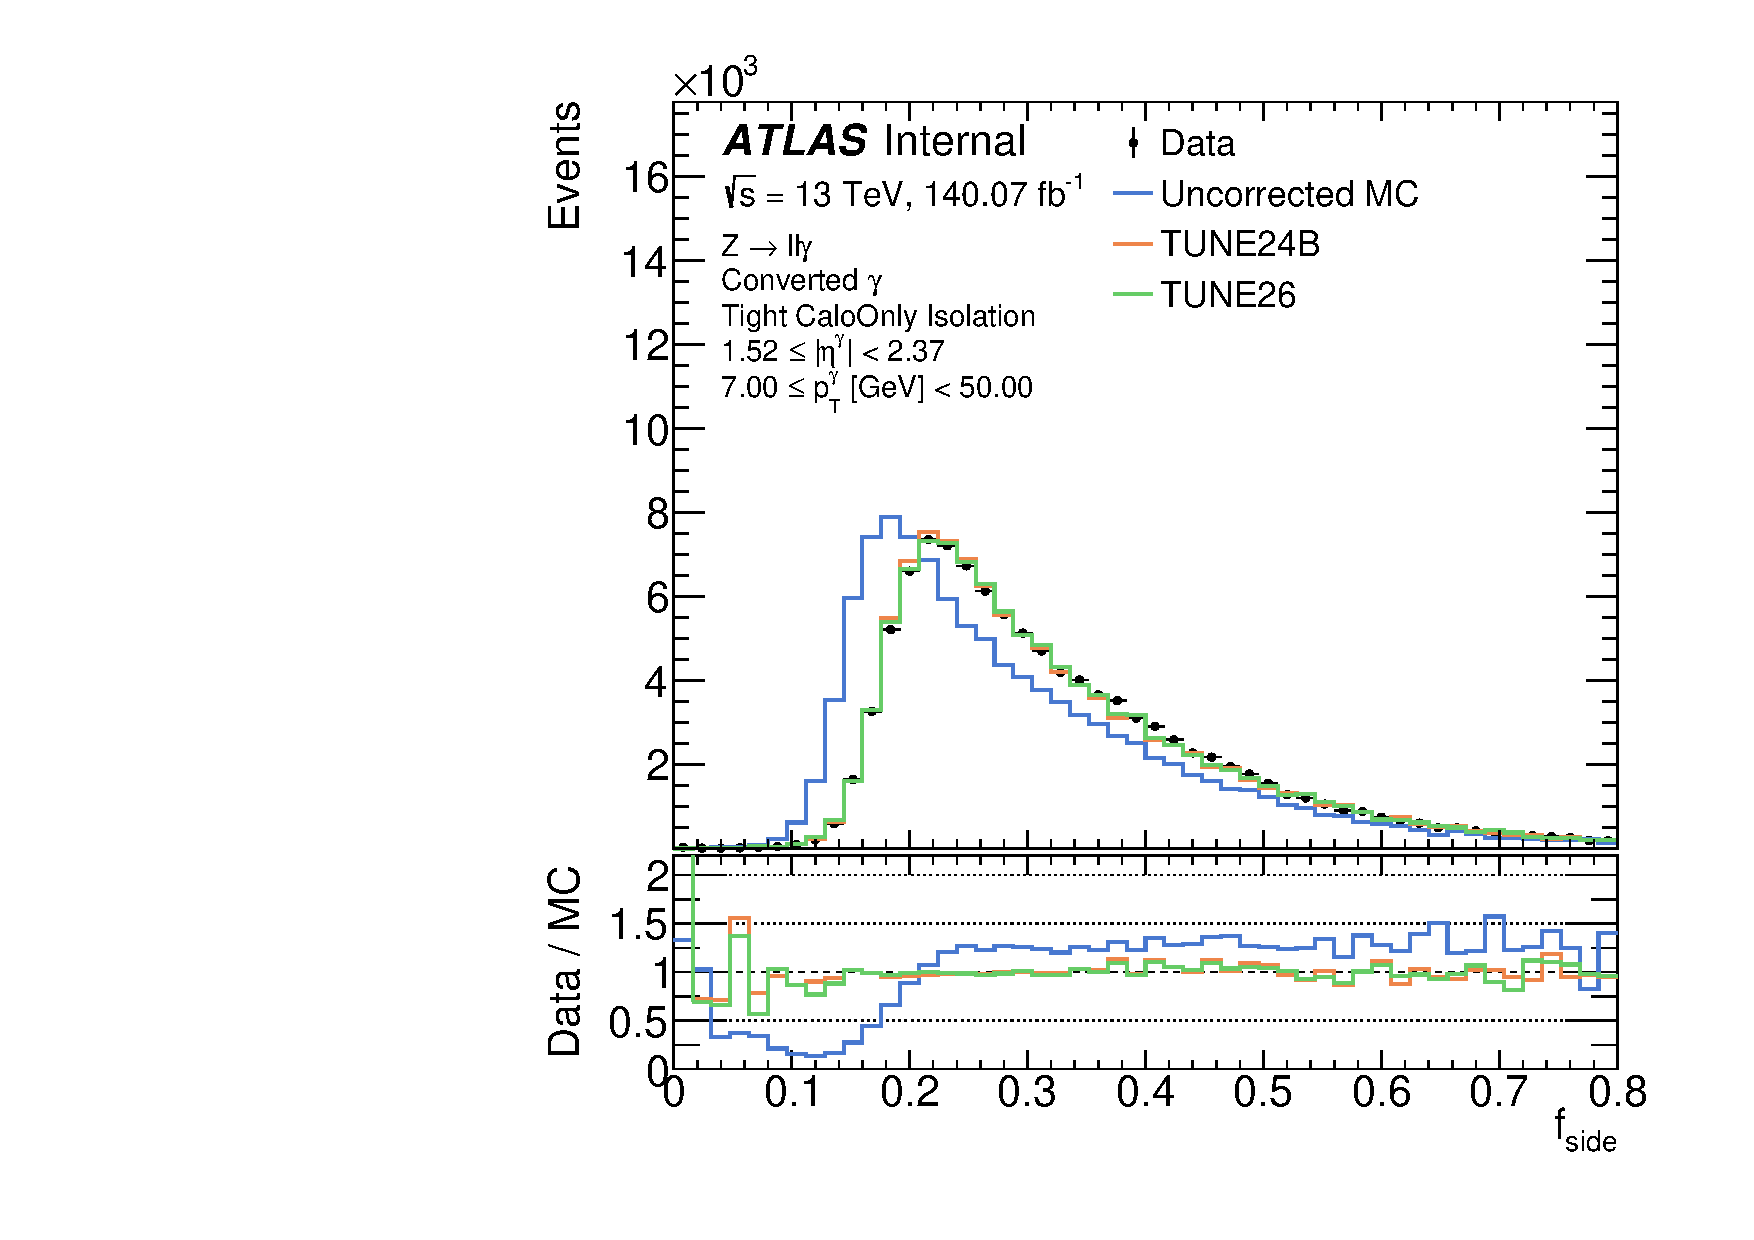
\includegraphics[width=\linewidth]{4_photonid/ffs/results/RZ/corrections/c/ptFull/etaCoarse/can__correction__ph_fside__Isotightcaloonly_IdNone__c__ptFullpt07p0__etaCoarseeta1p52}
        \caption{\fside, endcap.}
    \end{subfigure}
    \hfill
    \begin{subfigure}[h]{0.32\linewidth}
        \centering
        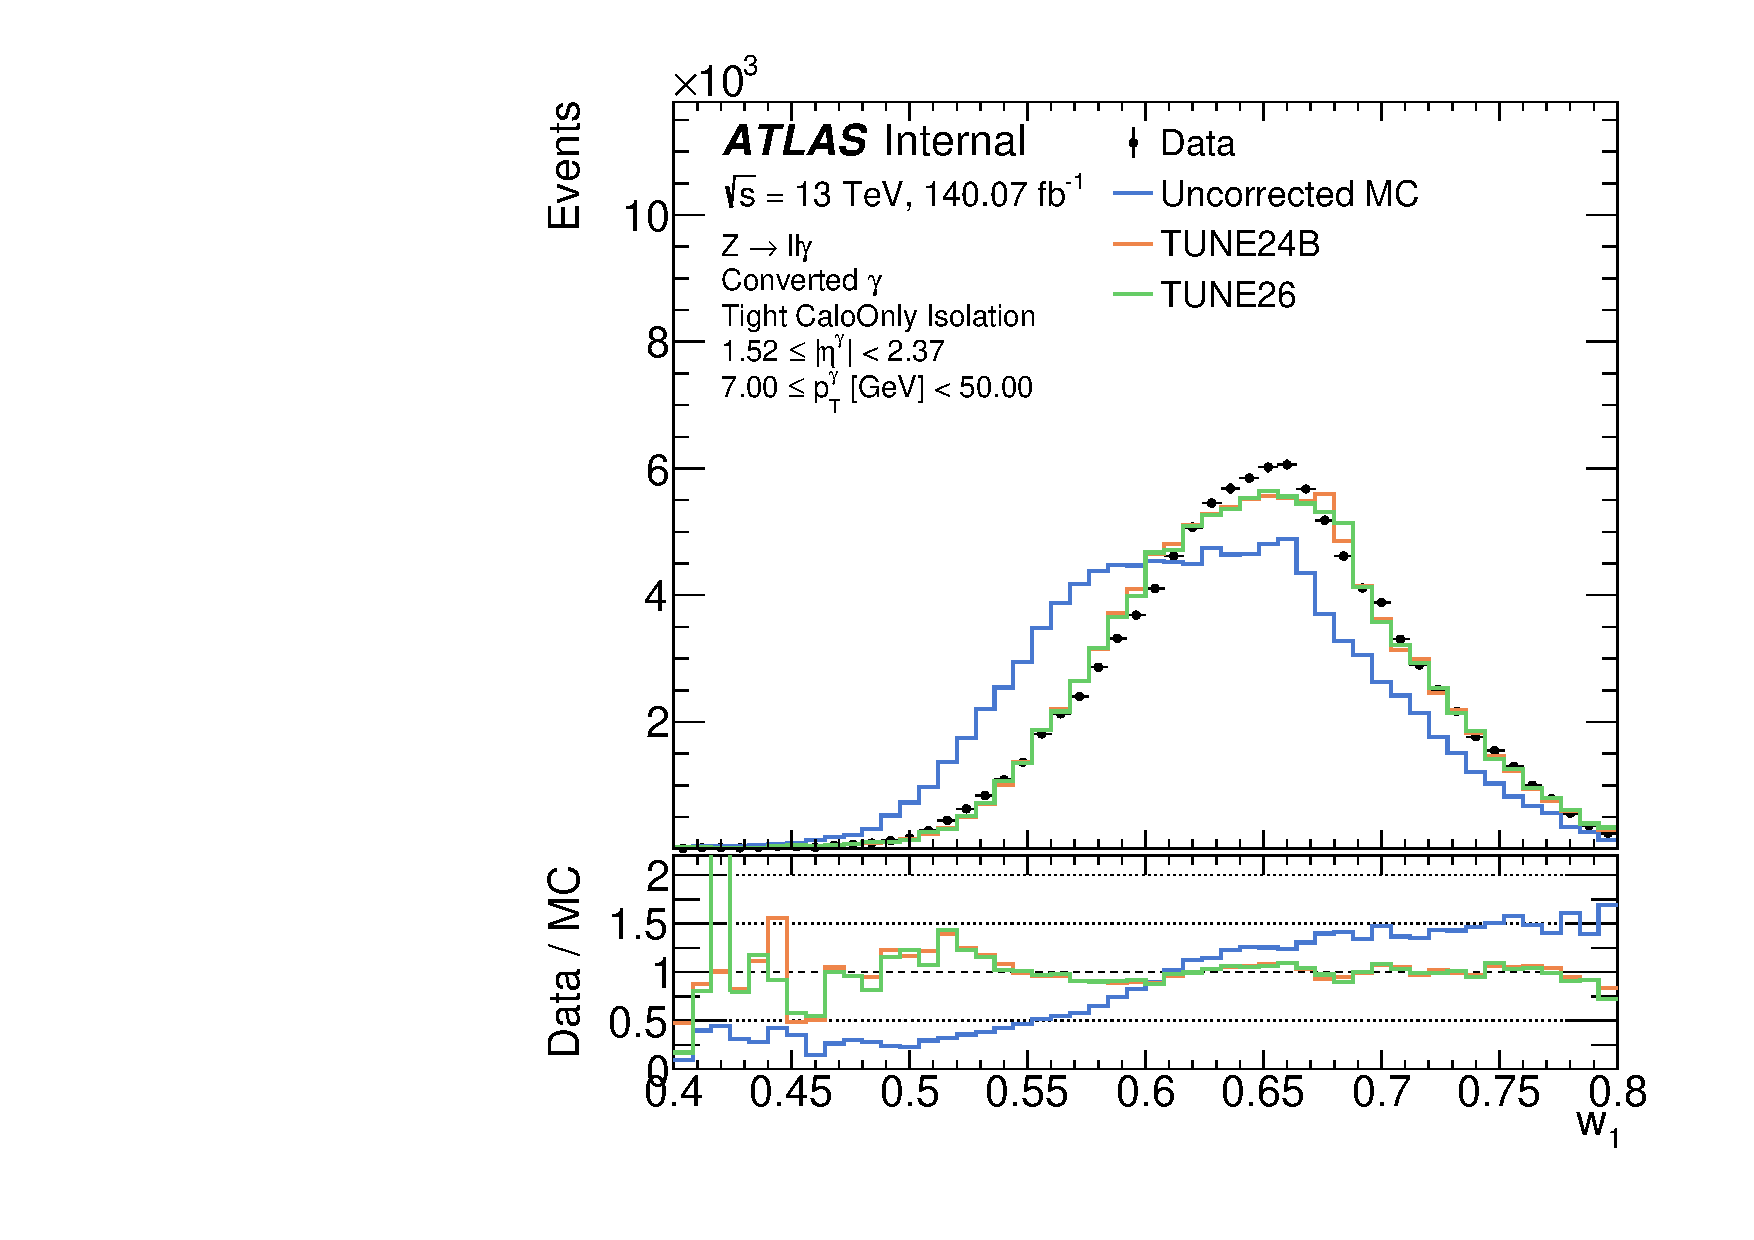
\includegraphics[width=\linewidth]{4_photonid/ffs/results/RZ/corrections/c/ptFull/etaCoarse/can__correction__ph_w1__Isotightcaloonly_IdNone__c__ptFullpt07p0__etaCoarseeta1p52}
        \caption{\wone, endcap.}
    \end{subfigure}
    \hfill
    \begin{subfigure}[h]{0.32\linewidth}
        \centering
        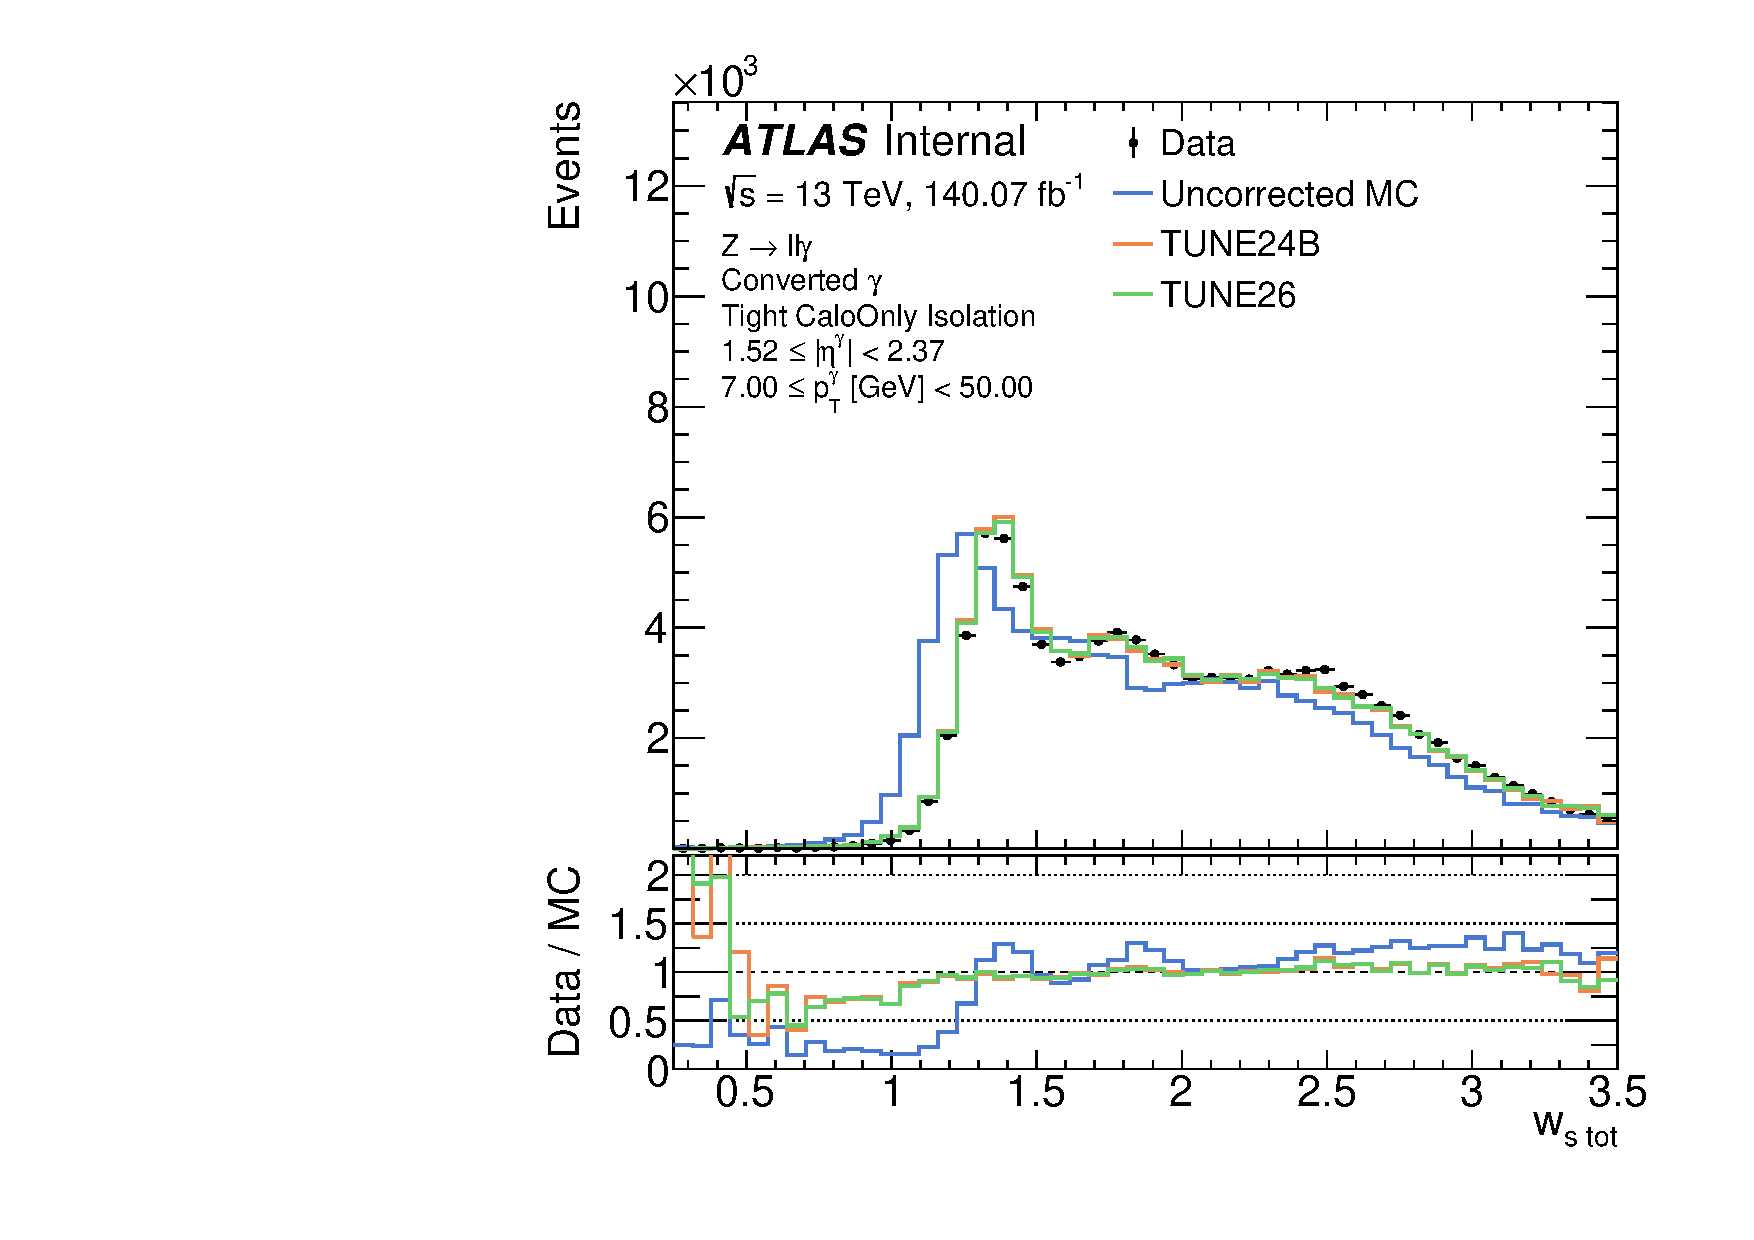
\includegraphics[width=\linewidth]{4_photonid/ffs/results/RZ/corrections/c/ptFull/etaCoarse/can__correction__ph_wstot__Isotightcaloonly_IdNone__c__ptFullpt07p0__etaCoarseeta1p52}
        \caption{\wstot, endcap.}
    \end{subfigure}\\
    \caption{Distribuciones de algunas \acp{SS} seleccionadas usando las muestras de \ac{RZ} para fotones convertidos luego de aplicar las correcciones de los \acp{FF} en la simulación. Las distribuciones de las \ac{SS} están separadas para fotones en la región del barrel (fila de arriba) y en la región del endcap (fila de abajo). Los puntos negros representan los datos recolectados por \ac{ATLAS}, mientras que las simulaciones no corregidas y corregidas están mostradas por las líneas azules y verdes, respectivamente. El panel inferior muestra el cociente entre el histograma de datos con cada uno de los obtenidos de las simulaciones \ac{MC}.}
    \label{fig:ss_corrections:ffs:results:ss_rz}
\end{figure}

\begin{figure}[ht!]
    \centering
    \begin{subfigure}[h]{0.32\linewidth}
        \centering
        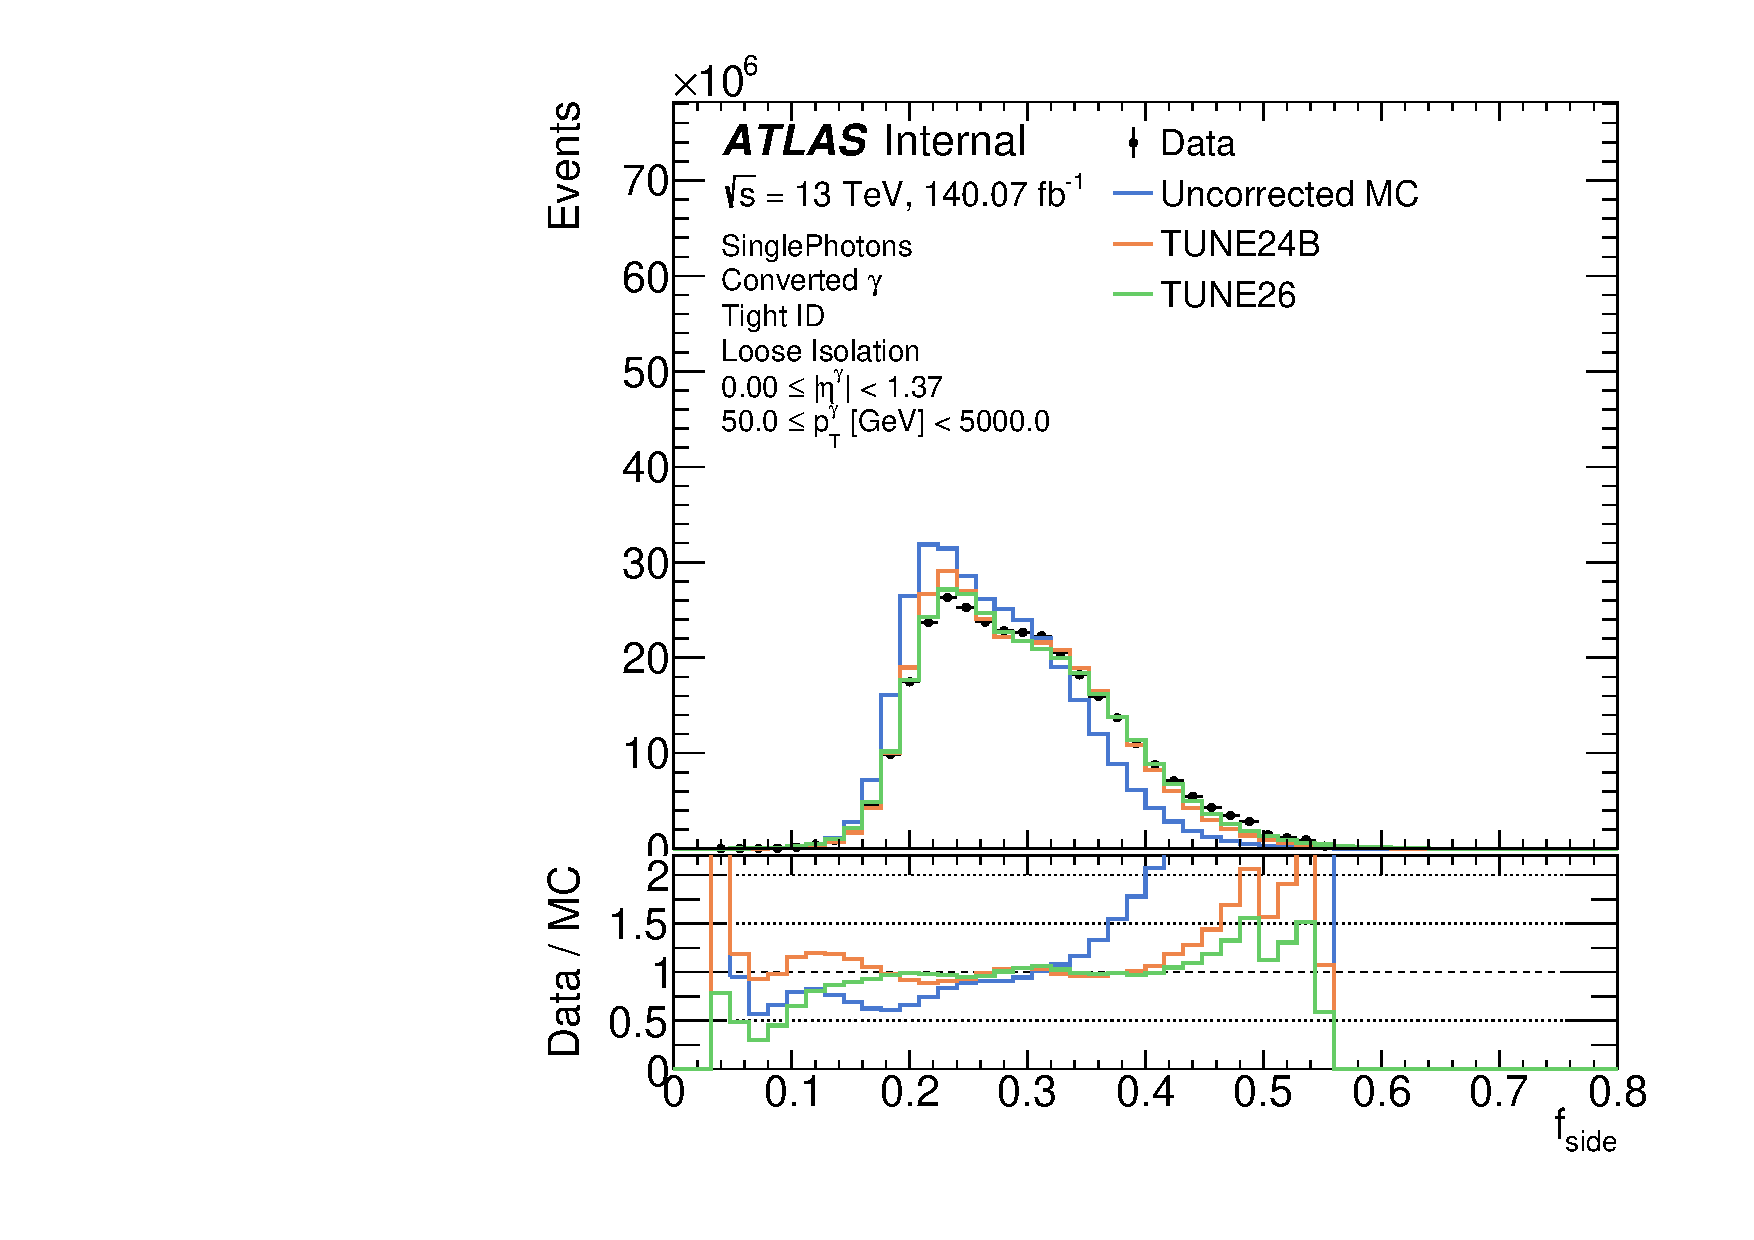
\includegraphics[width=\linewidth]{4_photonid/ffs/results/SP/corrections/c/ptFull/etaCoarse/can__correction__ph_fside__Isoloose_Idtight__c__ptFullpt0050p0__etaCoarseeta0p00}
        \caption{\fside, barrel.}
    \end{subfigure}
    \hfill
    \begin{subfigure}[h]{0.32\linewidth}
        \centering
        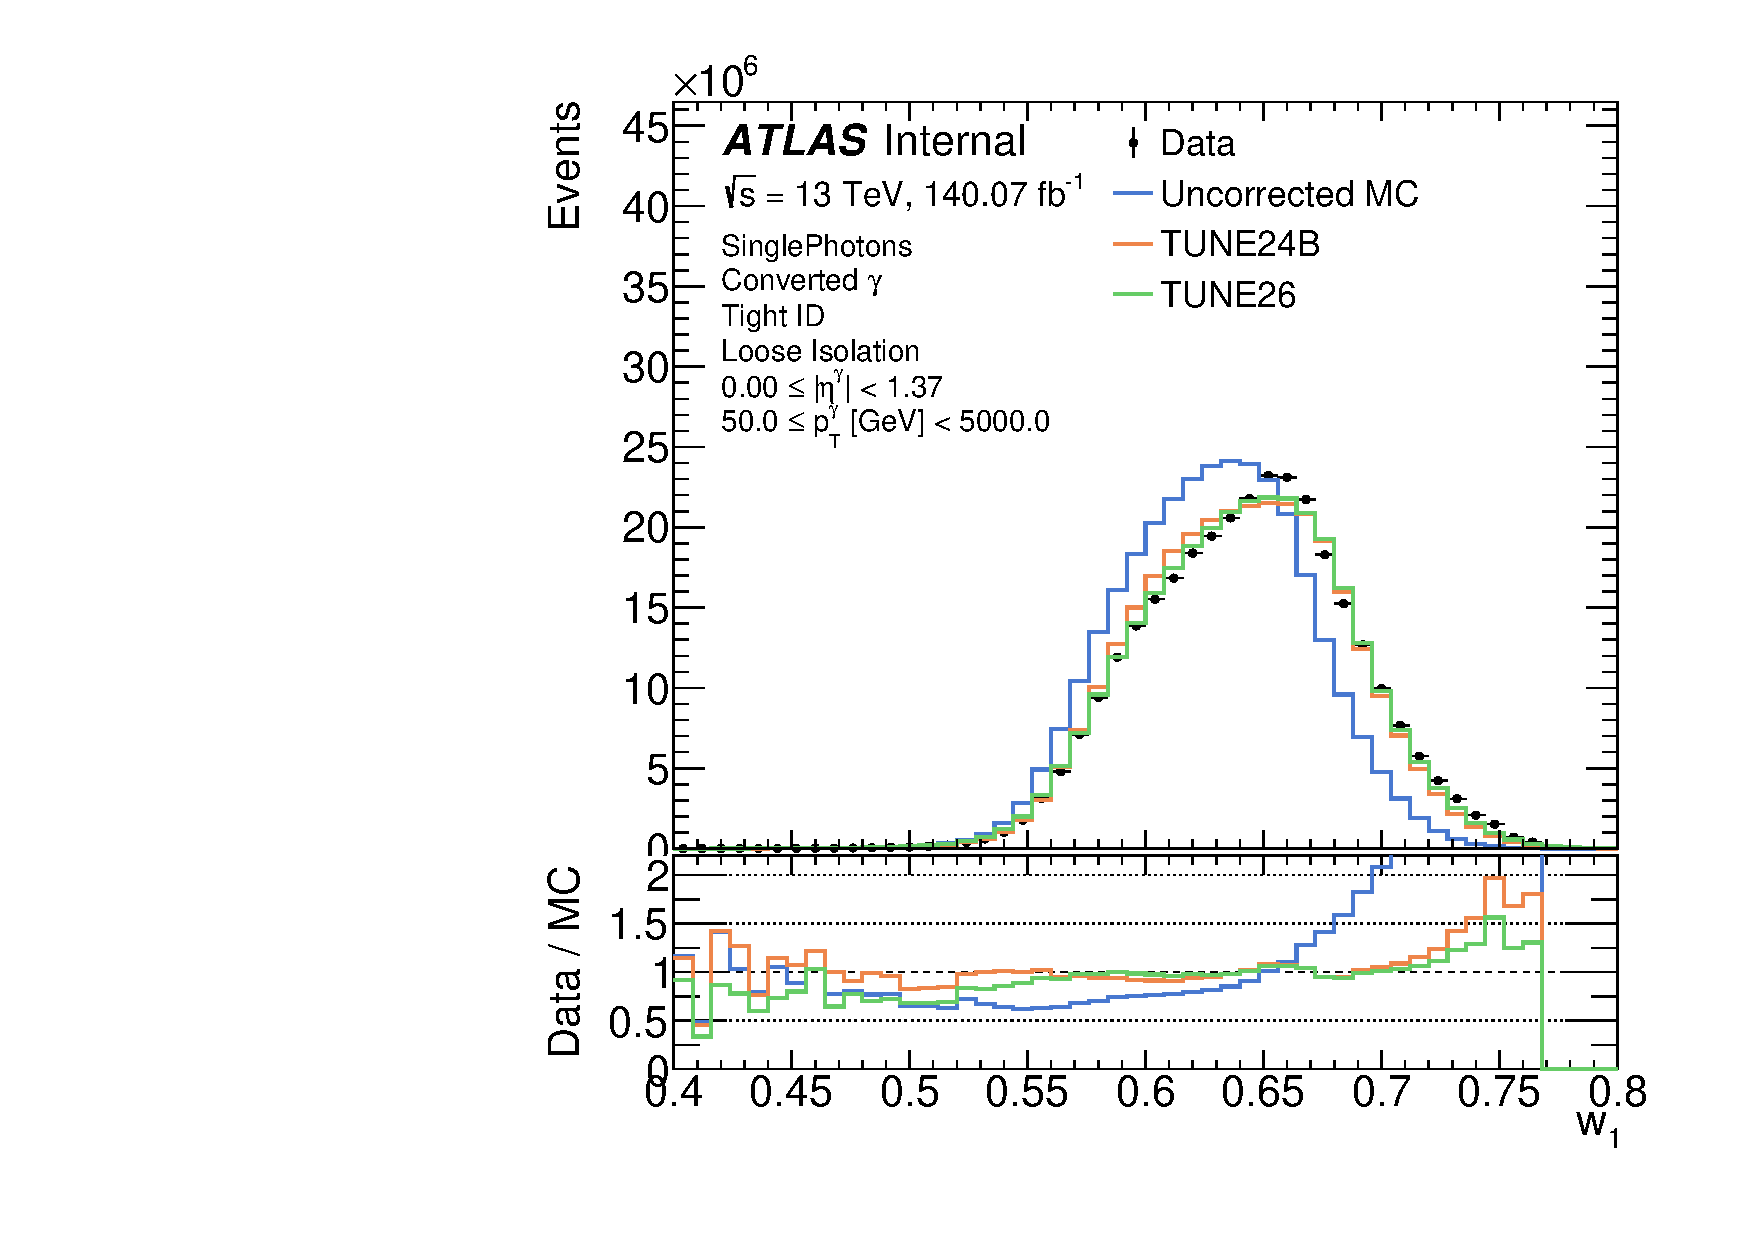
\includegraphics[width=\linewidth]{4_photonid/ffs/results/SP/corrections/c/ptFull/etaCoarse/can__correction__ph_w1__Isoloose_Idtight__c__ptFullpt0050p0__etaCoarseeta0p00}
        \caption{\wone, barrel.}
    \end{subfigure}
    \hfill
    \begin{subfigure}[h]{0.32\linewidth}
        \centering
        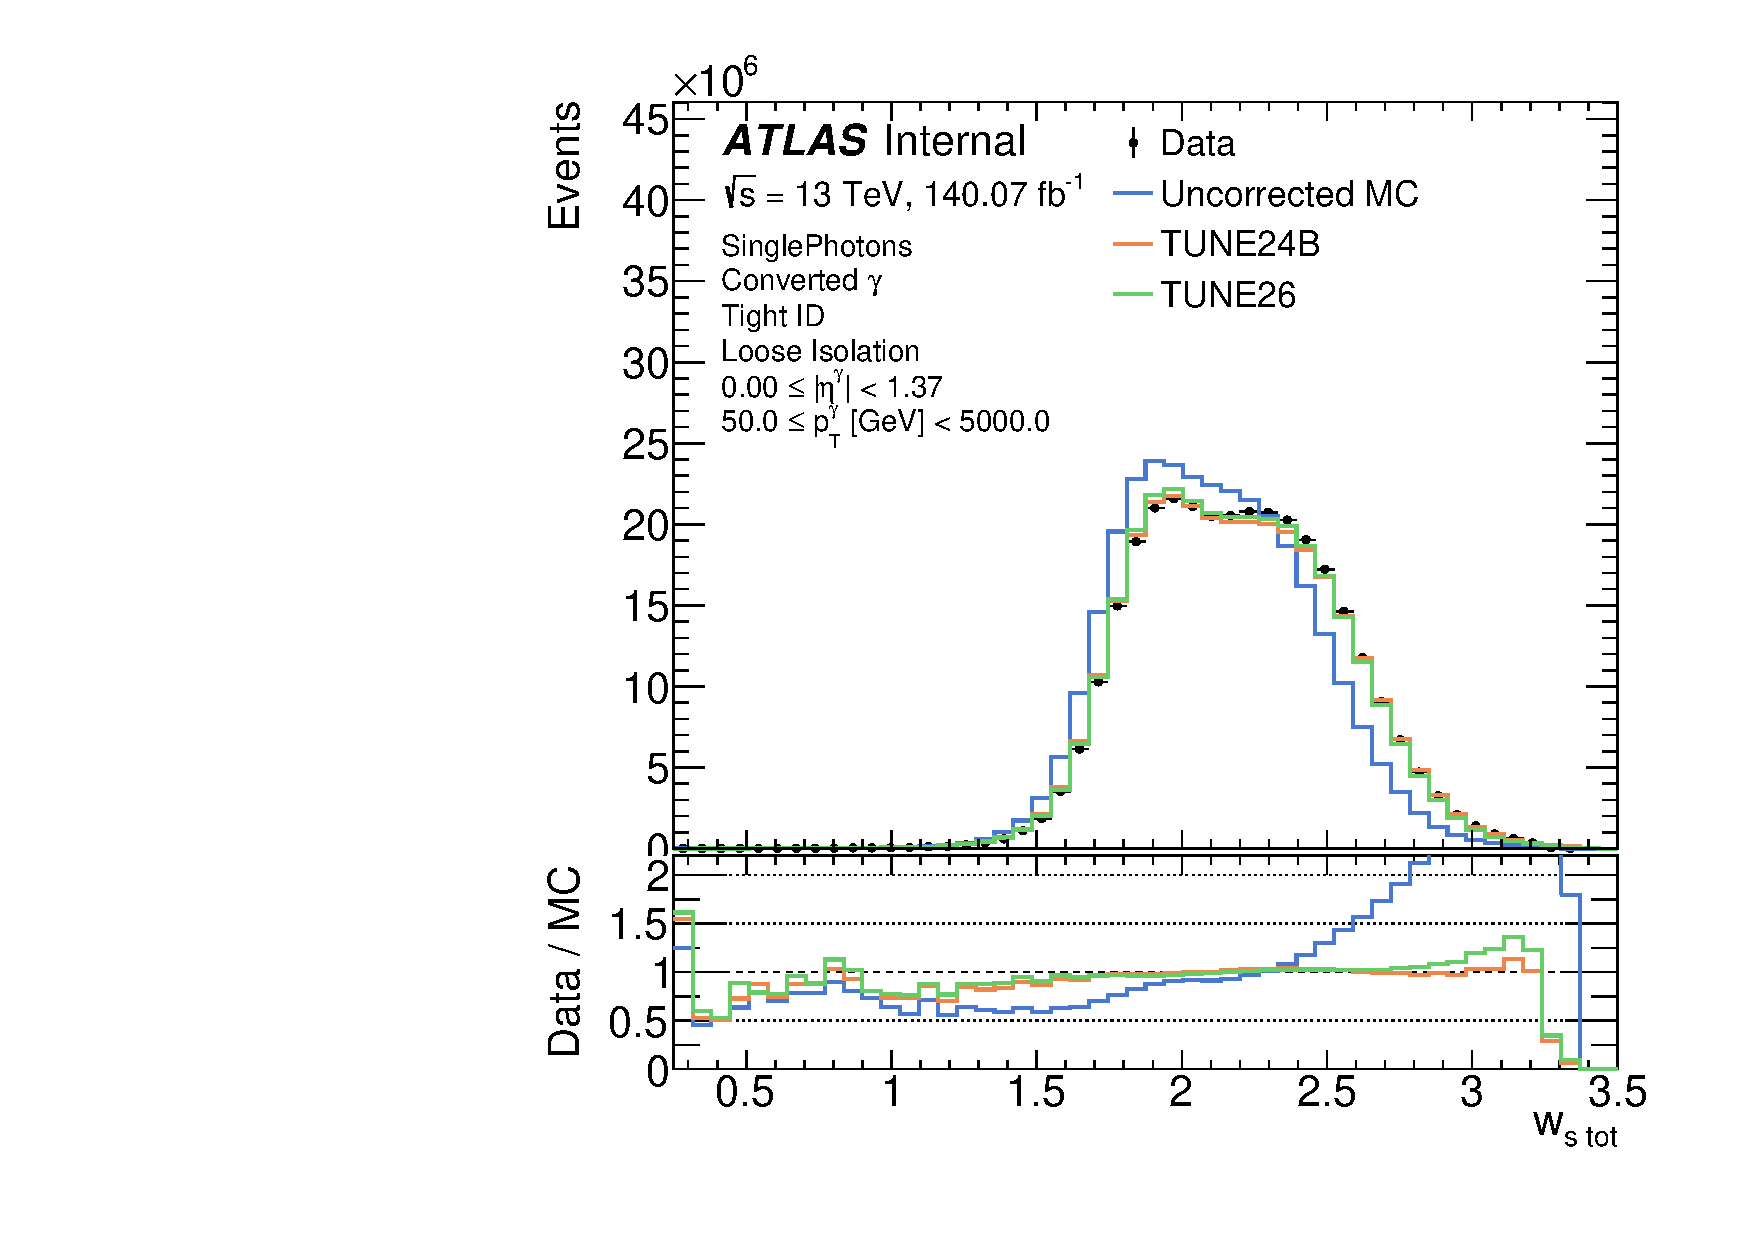
\includegraphics[width=\linewidth]{4_photonid/ffs/results/SP/corrections/c/ptFull/etaCoarse/can__correction__ph_wstot__Isoloose_Idtight__c__ptFullpt0050p0__etaCoarseeta0p00}
        \caption{\wstot, barrel.}
    \end{subfigure}\\
    \begin{subfigure}[h]{0.32\linewidth}
        \centering
        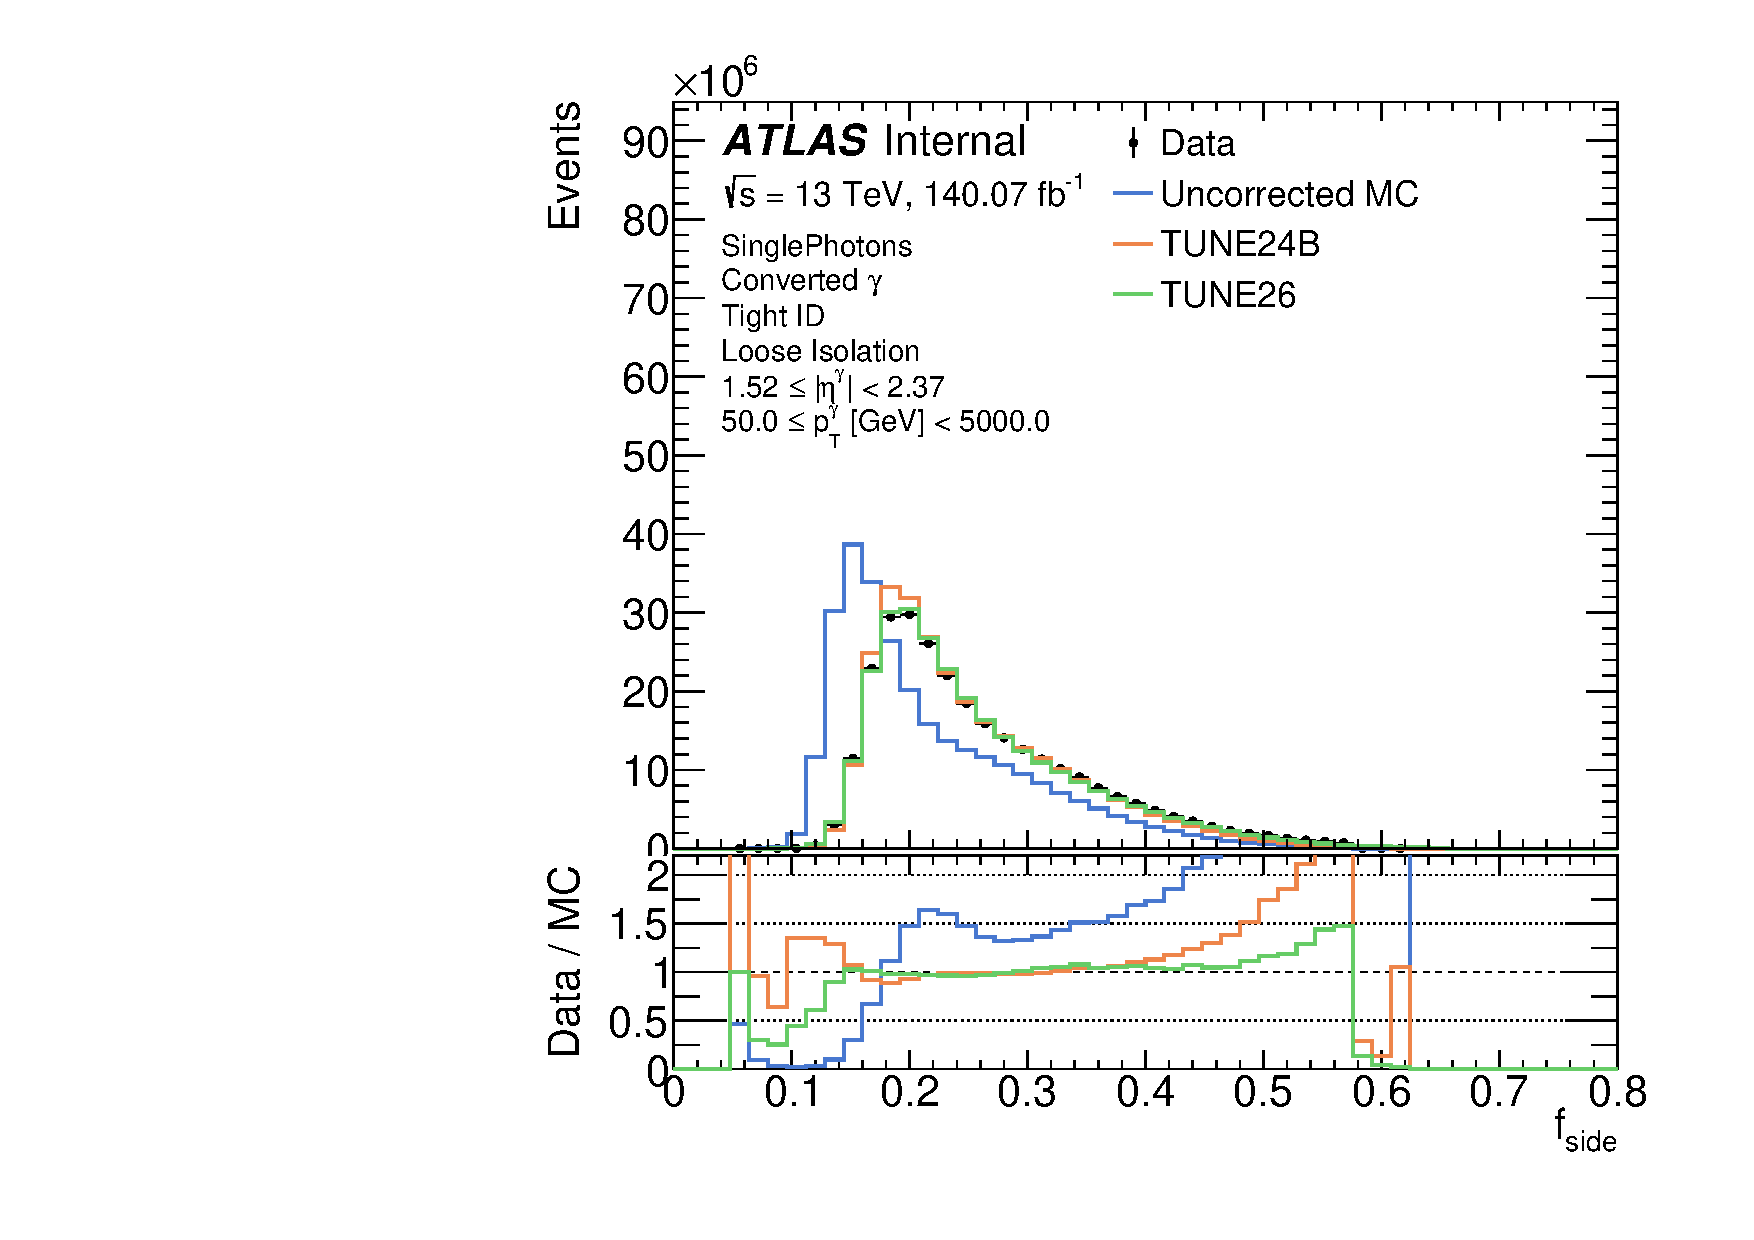
\includegraphics[width=\linewidth]{4_photonid/ffs/results/SP/corrections/c/ptFull/etaCoarse/can__correction__ph_fside__Isoloose_Idtight__c__ptFullpt0050p0__etaCoarseeta1p52}
        \caption{\fside, endcap.}
    \end{subfigure}
    \hfill
    \begin{subfigure}[h]{0.32\linewidth}
        \centering
        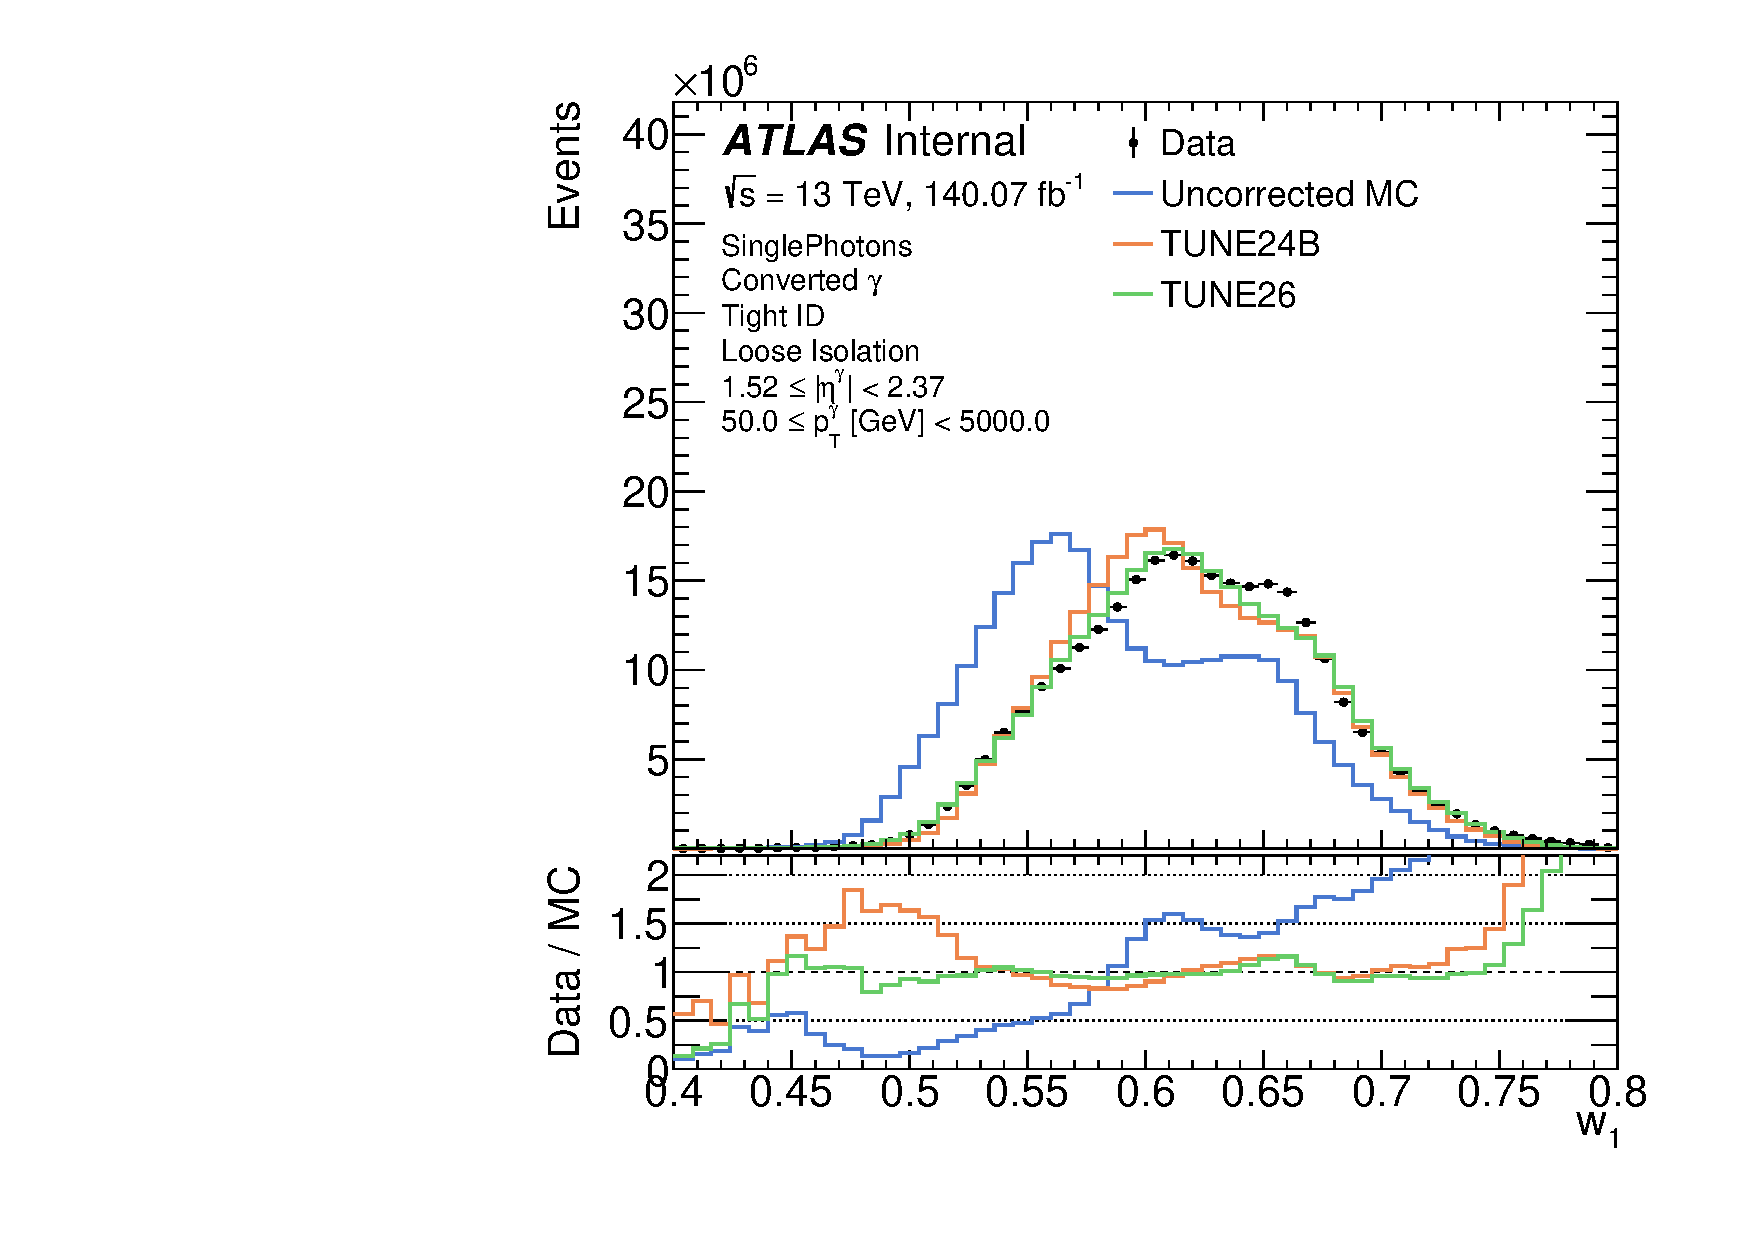
\includegraphics[width=\linewidth]{4_photonid/ffs/results/SP/corrections/c/ptFull/etaCoarse/can__correction__ph_w1__Isoloose_Idtight__c__ptFullpt0050p0__etaCoarseeta1p52}
        \caption{\wone, endcap.}
    \end{subfigure}
    \hfill
    \begin{subfigure}[h]{0.32\linewidth}
        \centering
        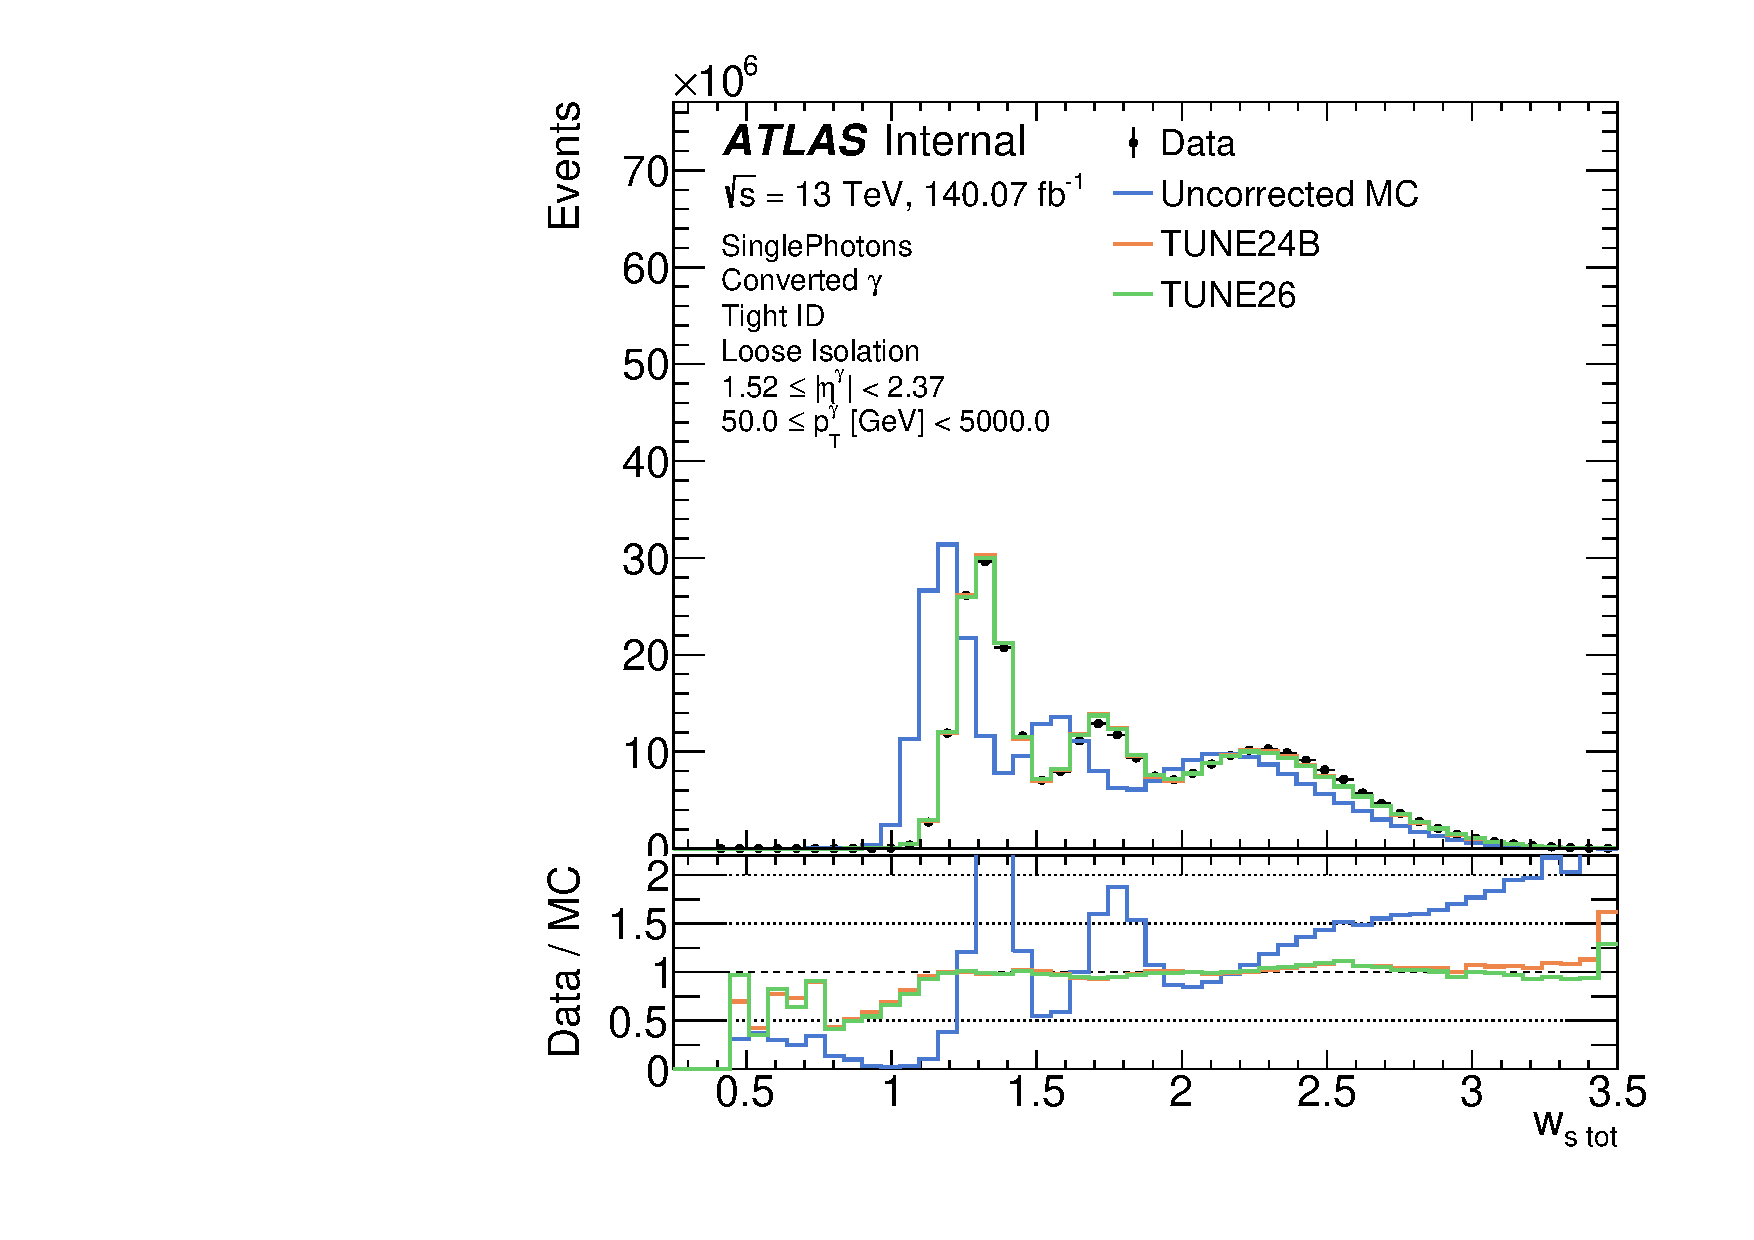
\includegraphics[width=\linewidth]{4_photonid/ffs/results/SP/corrections/c/ptFull/etaCoarse/can__correction__ph_wstot__Isoloose_Idtight__c__ptFullpt0050p0__etaCoarseeta1p52}
        \caption{\wstot, endcap.}
    \end{subfigure}\\
    \caption{Ídem a la \Fig{\ref{fig:ss_corrections:ffs:results:ss_rz}} pero utilizando las muestras de \ac{SP}.}
    \label{fig:ss_corrections:ffs:results:ss_sp}
\end{figure}
























\section{Correcciones de energía de las celdas}
\label{sec:ss_corrections:cell_rw}

El diseño y la funcionalidad del \ac{ECAL} de \ac{ATLAS} se describió en la \Sect{\ref{subsubsec:atlas:atlas:cals:ecal}}, así como el proceso a partir del cual los electrones y los fotones depositan sus energías en el \ac{ECAL}: creación de pares y radiación bremsstrahlung. Luego, a partir de estas deposiciones de energía en el \ac{ECAL} se construyen los \acp{SS} y se utilizan para la identificación de fotones. Sin embargo, el hecho de que las \acp{SS} calculadas mediante las simulación \ac{MC} y los datos no coincidan indica que las deposiciones de energía son diferentes, significando que el desacuerdo ocurre, en realidad, a un nivel inferior.

Aunque el método de \ac{FF} descripto anteriormente condujo a una excelente mejora del acuerdo entre los datos y las distribuciones \ac{MC}, sigue siendo una modificación en las variables de alto nivel y todas independientemente unas de otras. Un enfoque diferente consistía en modificar directamente los depósitos de energía de las celdas en la simulación \ac{MC}, corrigiendo todas las variables calculadas a partir de estas energías corregidas, incluidas las \acp{SS}.


El enfoque de corregir las energías de las celdas del \ac{ECAL} se ha desarrollado y probado inicialmente para electrones~\cite{thesis_khandoga} y posteriormente para fotones~\cite{thesis_belfkir}. Para el caso de los electrones, los resultados han sido muy prometedores ya que se corrigieron sustancialmente las \acp{SS} de la segunda capa del calorímetro. Sin embargo, para fotones, el mismo método que se utilizó para los electrones no funcionó de la forma que se esperaba ya que sólo permitió corregir las energías en promedio.
% Otro enfoque para corregir la simulación se basó en hacer coincidir eventos de datos y eventos simulados, estudio que sólo fue probado pseudodatos y resulta técnicamente complicado, pero que condujo a mejores resultados~\cite{thesis_belfkir}.

En la presente sección se estudia una nueva forma de corregir las energías de las celdas en \ac{MC}~\cite{ATLAS-QT-Sili}. Por simplicidad, en una primera etapa, se estudió solo la segunda capa del \ac{ECAL}. El método tiene similitudes con el método \ac{FF} lo que además facilita su comprensión.
% En primer lugar, se presenta la selección de eventos especiales utilizada para este estudio. Se discute brevemente el método de corrección de energías utilizado por los primeros estudios basados en electrones y fotones, y luego se presenta en detalle cómo se mejora este método.






\subsection{Cálculo de las correcciones}
\label{subsec:ss_corrections:cell_rw:calculation}


Los estudios presentados en esta sección se llevan a cabo con el mismo conjunto de datos utilizado para el cálculo \ac{FF}, descripto en la \Sect{\ref{subsec:ss_corrections:ffs:samples}}. Sin embargo, en este caso sólo se utilizan las muestras de \ac{RZ}.
Los eventos se seleccionan como se describe en la \Sect{\ref{subsec:pid_ss:pid:event_selection}}, utilizando fotones que pasan el criterio de aislamiento \texttt{Loose}.

Los electrones o fotones que atraviesan el \ac{ECAL} dejan su energía depositada en un conjunto de celdas. En este trabajo, utilizando la segunda capa del \ac{ECAL}, las celdas se agrupan en clusters de \(7\times 11\) celdas en \(\eta\times\phi\) y se encuentran centradas alrededor de la celda más energética. Esta disposición se puede observar en la \Fig{\ref{fig:ss_corrections:cell_rw:event_selection:cluster:arrangement}}. Aproximadamente el \(90\%\) de la energía del cluster se reparte entre las 9 celdas centrales, resaltadas en azul en la \Fig{\ref{fig:ss_corrections:cell_rw:event_selection:cluster:arrangement}}. La energía media normalizada de los datos se muestra en la \Fig{\ref{fig:ss_corrections:cell_rw:event_selection:cluster:energy}} visualizando cómo se distribuye la energía.

\begin{figure}[ht!]
    \centering
    \begin{subfigure}[t]{0.49\linewidth}
        \centering
        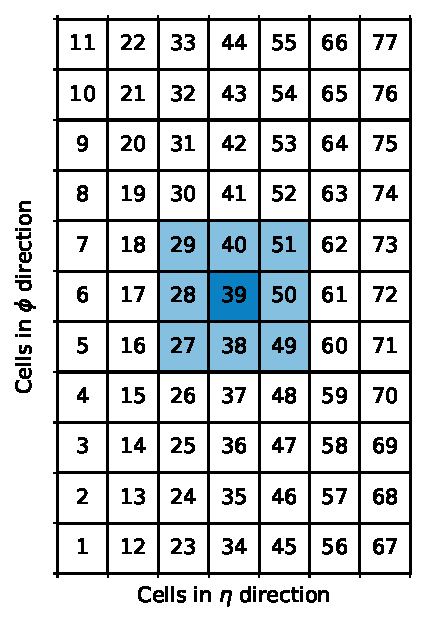
\includegraphics[width=0.5\linewidth]{4_photonid/cell_rw/cells_visualization}
        \caption{Disposición de las celdas, mostrando para cada una su número. La celda central corresponde a la celda número 39 resaltada en azul oscuro, mientras que las 8 celdas vecinas se muestran resaltadas en celeste.}
        \label{fig:ss_corrections:cell_rw:event_selection:cluster:arrangement}
    \end{subfigure}
    \hfill
    \begin{subfigure}[t]{0.49\linewidth}
        \centering
        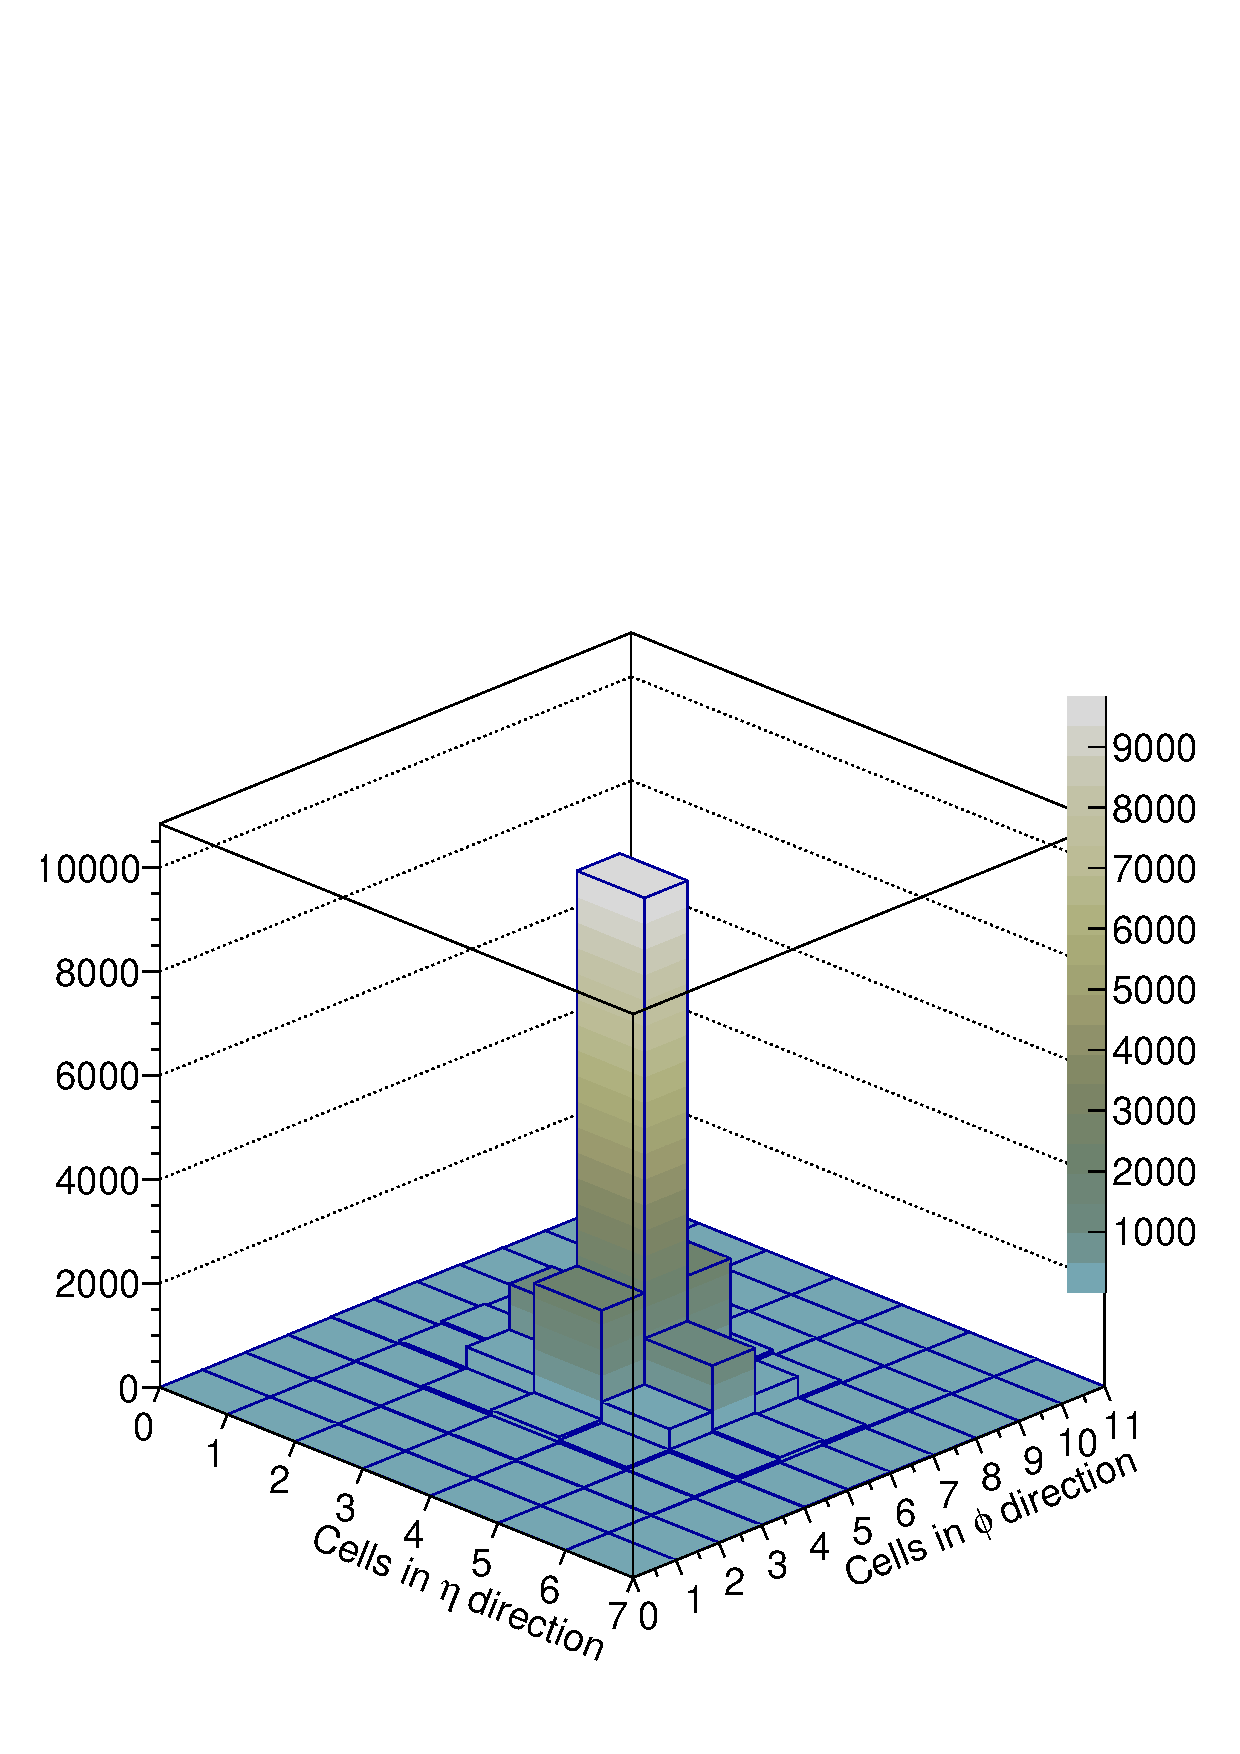
\includegraphics[width=0.8\linewidth]{4_photonid/cell_rw/cells-energy-u-etainclusive}
        \caption{Energía promedio en cada celda.}
        \label{fig:ss_corrections:cell_rw:event_selection:cluster:energy}
    \end{subfigure}
    \caption{Disposición de las celdas y distribución de la energía entre las celdas del cluster.}
    \label{fig:ss_corrections:cell_rw:event_selection:cluster}
\end{figure}


\subsubsection{Primeros pasos}
\label{subsubsec:ss_corrections:cell_rw:calculation:previous}

Todos los eventos que superen la selección mencionada tendrán asociados un cluster, cada uno de los cuales tendrá \(N\) celdas y cada celda tendrá una energía \(E_i\), con \(i=1,\dots,N\). Para cada evento, en primer lugar, se obtiene la energía total del cluster \(E\) sumando las energías de cada una de las celdas \(E_i\).
El método de las correcciones de las \acp{SS} mediante la corrección de las energías depositadas en el \ac{ECAL} hace uso de las energías normalizadas en cada celda, \(e_i = E_i/E\). Estos valores son la proporción de la energía total depositada que tiene una celda en particular.

El proceso de corrección comienza entonces calculando el valor medio de las distribuciones \(e_i\) (obtenidas una vez que todas los eventos pasan la selección) para la \(i\)-ésima celda, en la simulación \ac{MC} y en los datos, y la diferencia entre estos valores dan lugar a la corrección \(\Delta_i\) en dicha celda:
\begin{equation}
    \label{eq:ss_corrections:cell_rw:calculation:previous:old_corrections}
    \Delta_i = \overline{\left( \frac{ E_i^{\text{data}} }{ E^{\text{data}} } \right)} - \overline{\left( \frac{ E_i^{\text{MC}} }{ E^{\text{MC}} } \right)}
    = \bar e_i^{\text{data}} - \bar e_i^{\text{MC}}.
\end{equation}
Los valores \(E^{\text{data/MC}}\) son las energías totales del cluster para los datos y \ac{MC}, respectivamente.

La energía de la celda \(i\) se corrige entonces como
\begin{equation}
    \label{eq:ss_corrections:cell_rw:calculation:previous:correction_method}
    E_i^{\text{MC-RW}} = E_i^{\text{MC}} + \Delta_i E^{\text{MC}},
\end{equation}
que se traduce en desplazar la energía normalizada de la celda \(e_i^{\text{MC}}\) en una cantidad \(\Delta_i\) para que los valores medios de las distribuciones de \(e_i\) de datos y \ac{MC} coincidan. 

También es importante notar que, por definición, estos coeficientes de corrección suman 0 en todo el cluster:
\begin{equation*}
    \sum_i \Delta_i = \sum_i \overline{\left( \frac{ E_i^{\text{data}} }{ E^{\text{data}} } \right)} - \sum_i \overline{\left( \frac{ E_i^{\text{MC}} }{ E^{\text{MC}} } \right)}
    = \overline{\sum_i \frac{ E_i^{\text{data}} }{ E^{\text{data}} }} - \overline{\sum_i \frac{ E_i^{\text{MC}} }{ E^{\text{MC}} }}
    = 1 - 1 = 0,
\end{equation*}
implicando que el cambio de energía total del cluster se mantiene constante:
\begin{equation*}
    E^{\text{MC-RW}} \equiv \sum_i E_i^{\text{MC-RW}}
    = \sum_i E_i^{\text{MC}} + \sum_i \Delta_i E^{\text{MC}} = E^{\text{MC}} + E^{\text{MC}} \sum_i \Delta_i = E^{\text{MC}}.
\end{equation*}
Este hecho es de vital importancia ya que no se desea cambiar la energía total del cluster en la simulación \ac{MC} sino que se desea lograr una redistribución de la energía entre las celdas, de forma tal que cada una se asemeje a la de los datos.

Los coeficientes de corrección resultantes para cada celda en clusters de 77 celdas se pueden visualizar en la \Fig{\ref{fig:ss_corrections:cell_rw:calculation:previous:reweights}}. Como se puede notar de los valores mostrados, la celda central presenta una corrección negativa mientras que las 8 vecinas a la central tienen correcciones positivas. Esto se puede traducir a que, en la simulación, la celda central suele tener más energía en promedio que en los datos, mientras que lo opuesto ocurre en las vecinas. Mediante la aplicación de una corrección negativa (un corrimiento negativo de \(e_i\)) se remueve energía de la celda central que luego es distribuída en las circundantes.

\begin{figure}[htbp]
    \centering
    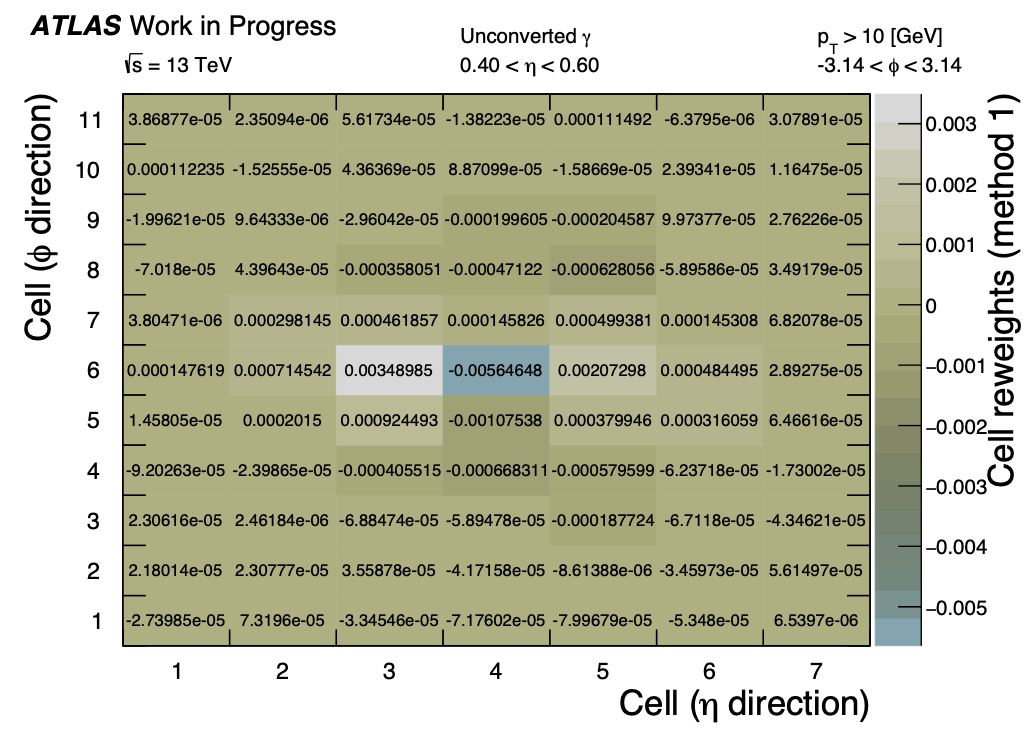
\includegraphics[width=0.6\linewidth]{4_photonid/cell_rw/old_method/reweights_method1u_ptInclusive_eta040_phiInclusive.png}
    \caption{Correcciones a las energías de las celdas de la simulación \ac{MC} utilizando el mismo método diseñado para electrones.}
    \label{fig:ss_corrections:cell_rw:calculation:previous:reweights}
\end{figure}

A partir de las energías de las celdas, se pueden calcular las \acp{SS} de la segunda capa del \ac{ECAL}, las cuales son \reta, \rphi y \weta:
\begin{gather*}
    \reta = \frac{E_{3\times 7}}{E_{7\times 7}}\\
    \rphi = \frac{E_{3\times 3}}{E_{7\times 3}}\\
    \weta = \sqrt{\frac{\sum_i E_i \eta^2_i}{\sum_i E_i} - \left( \frac{\sum_i E_i \eta_i}{\sum_i E_i} \right)^2}
\end{gather*}
donde \(E_{i\times j}\) es la energía de la celda sumada en una región de \(\eta\times\phi=i\times j\) celdas alrededor de la celda central. Se demostró en los estudios anteriores~\cite{thesis_belfkir} que este método sólo corrige las formas de las variables en promedio pero las diferencias en la forma permanecen. Esto se debe al hecho de que este método sólo corrige los valores medios de energía en las celdas. Sin embargo, estas distribuciones de energía siguen presentando diferencias, especialmente en lo que se refiere a las formas, lo que conduce a una situación muy similar a la observada para los \acp{FF}.
% De este modo, se puede emplear un enfoque muy similar para corregir los valores medios y los anchos de las distribuciones de energía normalizadas.
























\subsubsection{Nuevo método de corrección de energías}

Este nuevo método que se propone en esta tesis, pretende corregir tanto el valor medio como la varianza de las distribuciones normalizadas de energía de las celdas, mediante la aplicación de corrimientos (shift) y estiramientos (stretch) de las mismas. De forma similar al enfoque seguido para las \acp{SS} utilizando el método de \acp{FF}, una primera aproximación a los valores de shift y stretch de las distribuciones de energía consiste en calcular el valor medio y la raíz cuadrática media (RMS) de las mismas en cada celda, respectivamente.
Luego, la energía normalizada de la \(i\)-ésima celda se obtiene como:
\begin{equation}
    \label{eq:ss_corrections:cell_rw:calculation:new:normalized_e}
    e_i^{\text{MC-RW}} =
    \underbrace{\frac{\text{RMS}_{e,i}^{\text{data}}}{\text{RMS}_{e,i}^{\text{MC}}}}_{\text{stretch}} e_i^{\text{MC}}
    +
    \underbrace{\left(\bar e_i^{\text{data}} - \frac{\text{RMS}_{e,i}^{\text{data}}}{\text{RMS}_{e,i}^{\text{MC}}} \bar e_i^{\text{MC}}  \right)}_{\text{shift}},
\end{equation}
donde el subíndice \(e\) en los valores de RMS indica que estos se calculan a partir de las distribuciones de energía normalizadas y el índice \(i\) recorre todas las celdas del cluster. De la expresión anterior se pueden identificar nuevamente un factor de shift, que es una transformación constante de la energía normalizada, y un factor de stretch, lineal en la variable que se requiere corregir.

Dado que la energía normalizada en la celda \(i\) puede calcularse como \(e_i^{j} = E_i^{j} / E^{j}\) y que se requiere mantener la misma energía total del cluster constante (\(E^{\text{MC-RW}} = E^{\text{MC}}\)), se puede multiplicar la \Eqn{\ref{eq:ss_corrections:cell_rw:calculation:new:normalized_e}} por \(E^{\text{MC-RW}}\) y llegar a una expresión para \(E_i^{\text{MC-RW}}\):
\begin{equation}
    \label{eq:ss_corrections:cell_rw:calculation:new:correction_method}
    E_i^{\text{MC-RW}} =
    \frac{\text{RMS}_{e,i}^{\text{data}}}{\text{RMS}_{e,i}^{\text{MC}}} E_i^{\text{MC}}
    +
    \left( \bar e_i^{\text{data}} - \frac{\text{RMS}_{e,i}^{\text{data}}}{\text{RMS}_{e,i}^{\text{MC}}} \bar e_i^{\text{MC}} \right) E^{\text{MC}}.
\end{equation}
Por último, para garantizar que la energía del cluster permanezca constante, las energías de las celdas se normalizan por \(\sum_i E_i^{\text{MC}} / \sum_i E_i^{\text{MC-RW}}\).

Como el resultado de este procedimiento de corrección de energías involucra una corrección de shift y otra de stretch, se obtienen dos matrices de corrección y un ejemplo de ellas se presenta en la \Fig{\ref{fig:ss_corrections:cell_rw:calculation:new:reweights}}.
En lo que sigue, este nuevo método se aplica para corregir las energías de las celdas y se computa de forma inclusiva en \pt y \abseta, sólo separando entre fotones no convertidos y convertidos.

\begin{figure}[ht!]
    \centering
    \begin{subfigure}[h]{0.49\linewidth}
        \centering
        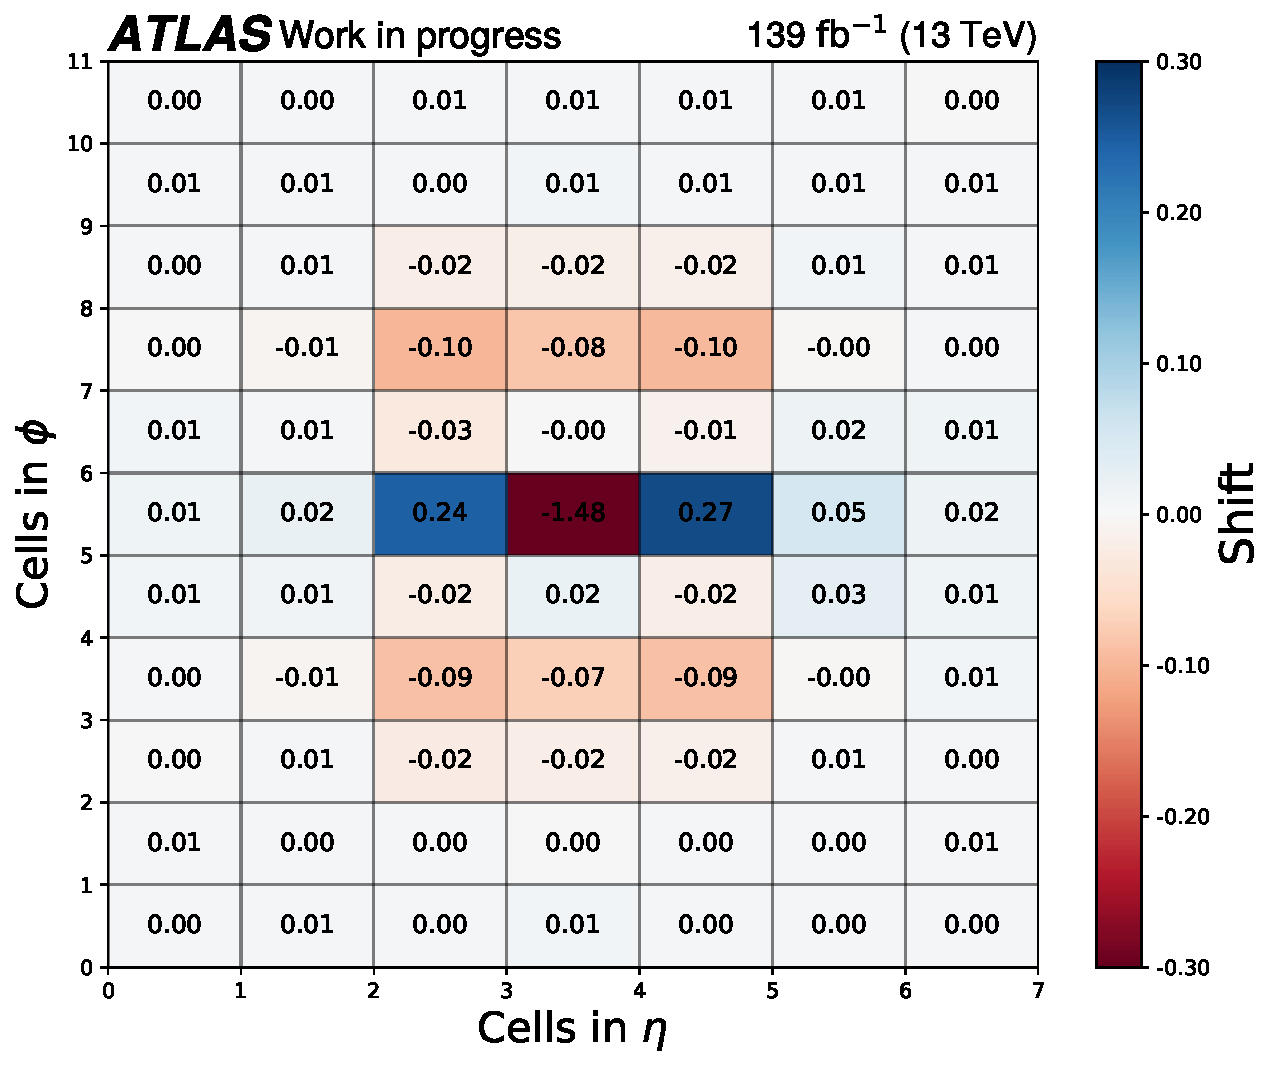
\includegraphics[width=\linewidth]{4_photonid/cell_rw/results/h_u_shift_mpl}
        \caption{Shift}
    \end{subfigure}
    \hfill
    \begin{subfigure}[h]{0.49\linewidth}
        \centering
        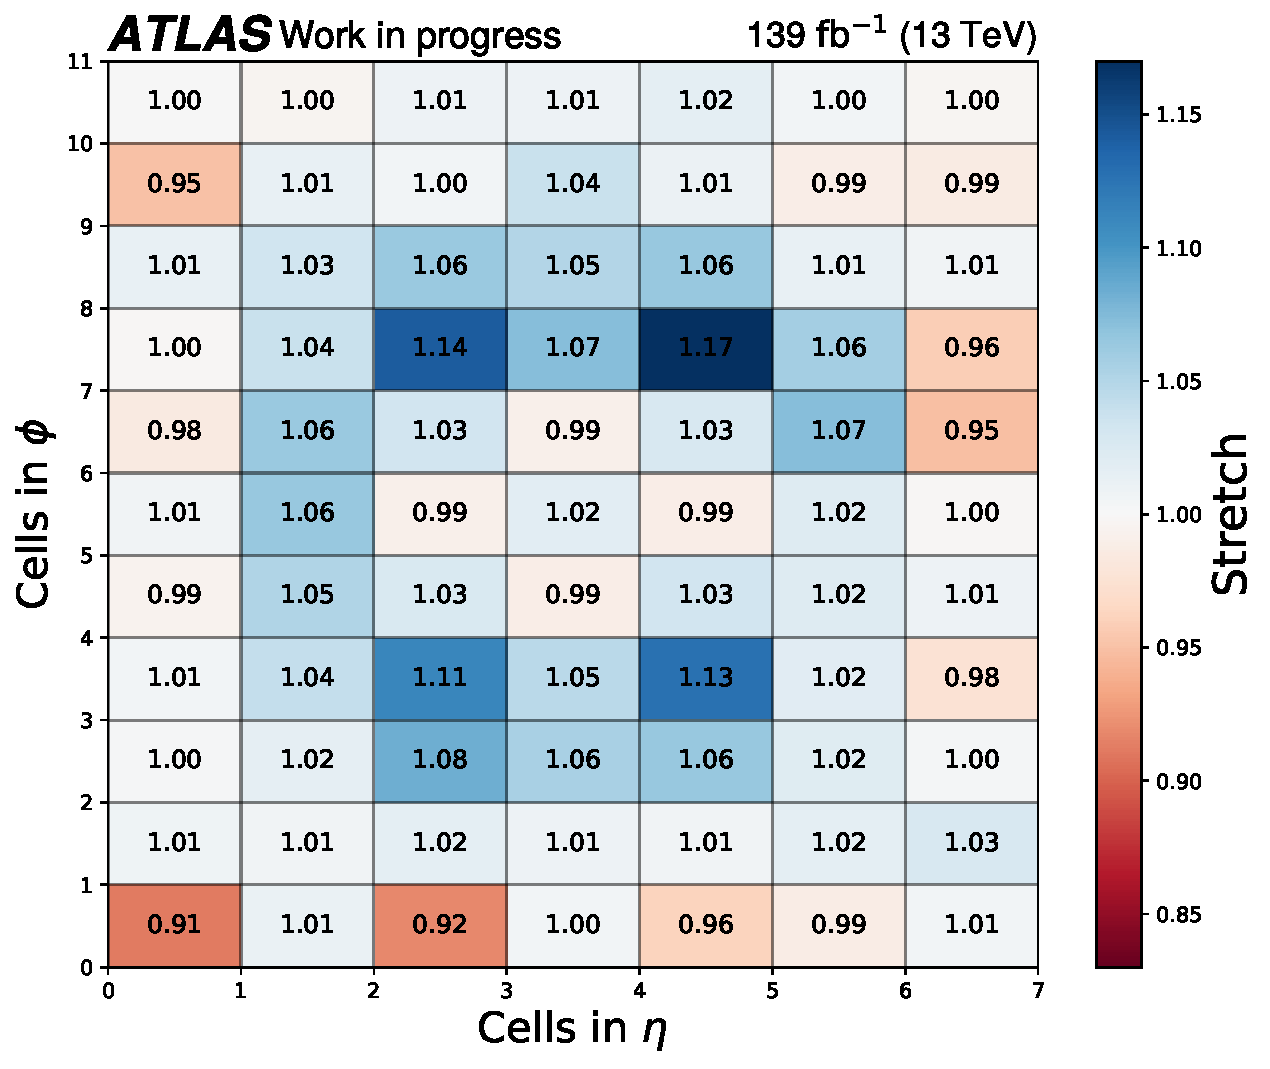
\includegraphics[width=\linewidth]{4_photonid/cell_rw/results/h_u_stretch_mpl}
        \caption{Stretch}
    \end{subfigure}
    \caption{Ejemplo de las matrices de corrección de shift (izquierda) y stretch (derecha). Los valores mostrados corresponden al cálculo de las correcciones utilizando fotones no convertidos. Los valores de shift son multiplicados por un factor de 100 para mejorar su visualización.}
    \label{fig:ss_corrections:cell_rw:calculation:new:reweights}
\end{figure}









\subsection{Resultados}
\label{subsec:ss_corrections:cell_rw:results}

La \Fig{\ref{fig:ss_corrections:cell_rw:calculation:new:reweights}} muestra las matrices de corrección de shift y stretch obtenidas para fotones no convertidos. Puede observarse que, al igual que en el caso del método anterior, la mayor corrección de shift se realiza en la celda central donde el shift corresponde a un valor negativo. De la misma forma que en el caso anterior, los shifts de las celdas vecinas en la dirección de \(\eta\) son positivos y grandes, indicando la redistribución de la energía de la celda central en estas dos vecinas.
Sin embargo, se puede notar que las segundas celdas vecinas en la dirección de \(\phi\) sufren una gran corrección, quitando energía mediante el shift pero aumentando también el ancho de la distribución dado por los estiramientos positivos. Del resto de las celdas del cluster se nota que no presentan corrimiento significativo, aunque presentan un stretch \(<1\) indicando que se hacen más angostas, especialmente las celdas de los extremos del cluster.

Utilizando estos factores de corrección para las energías normalizadas de cada celda, en las \Fig{\ref{fig:ss_corrections:cell_rw:results:cells}} se muestran las distribuciones de energía normalizadas resultantes para las celdas 28, 39 y 50~\footnote{Como fue mostrado en la \Fig{\ref{fig:ss_corrections:cell_rw:event_selection:cluster:arrangement}}, la celda número 39 es la central, mientras que las celdas 28 y 50 están a la izquierda y derecha, respectivamente, en la dirección \(\eta\).}. El nuevo método de corrección consigue grandes mejoras en el acuerdo entre los datos y la simulación. Además, el método logra corregir bien las colas de las distribuciones de todas las celdas así como los picos de las mismas, lo que puede observarse especialmente en la celda 28.

\begin{figure}[ht!]
    \centering
    \begin{subfigure}[h]{0.32\linewidth}
        \centering
        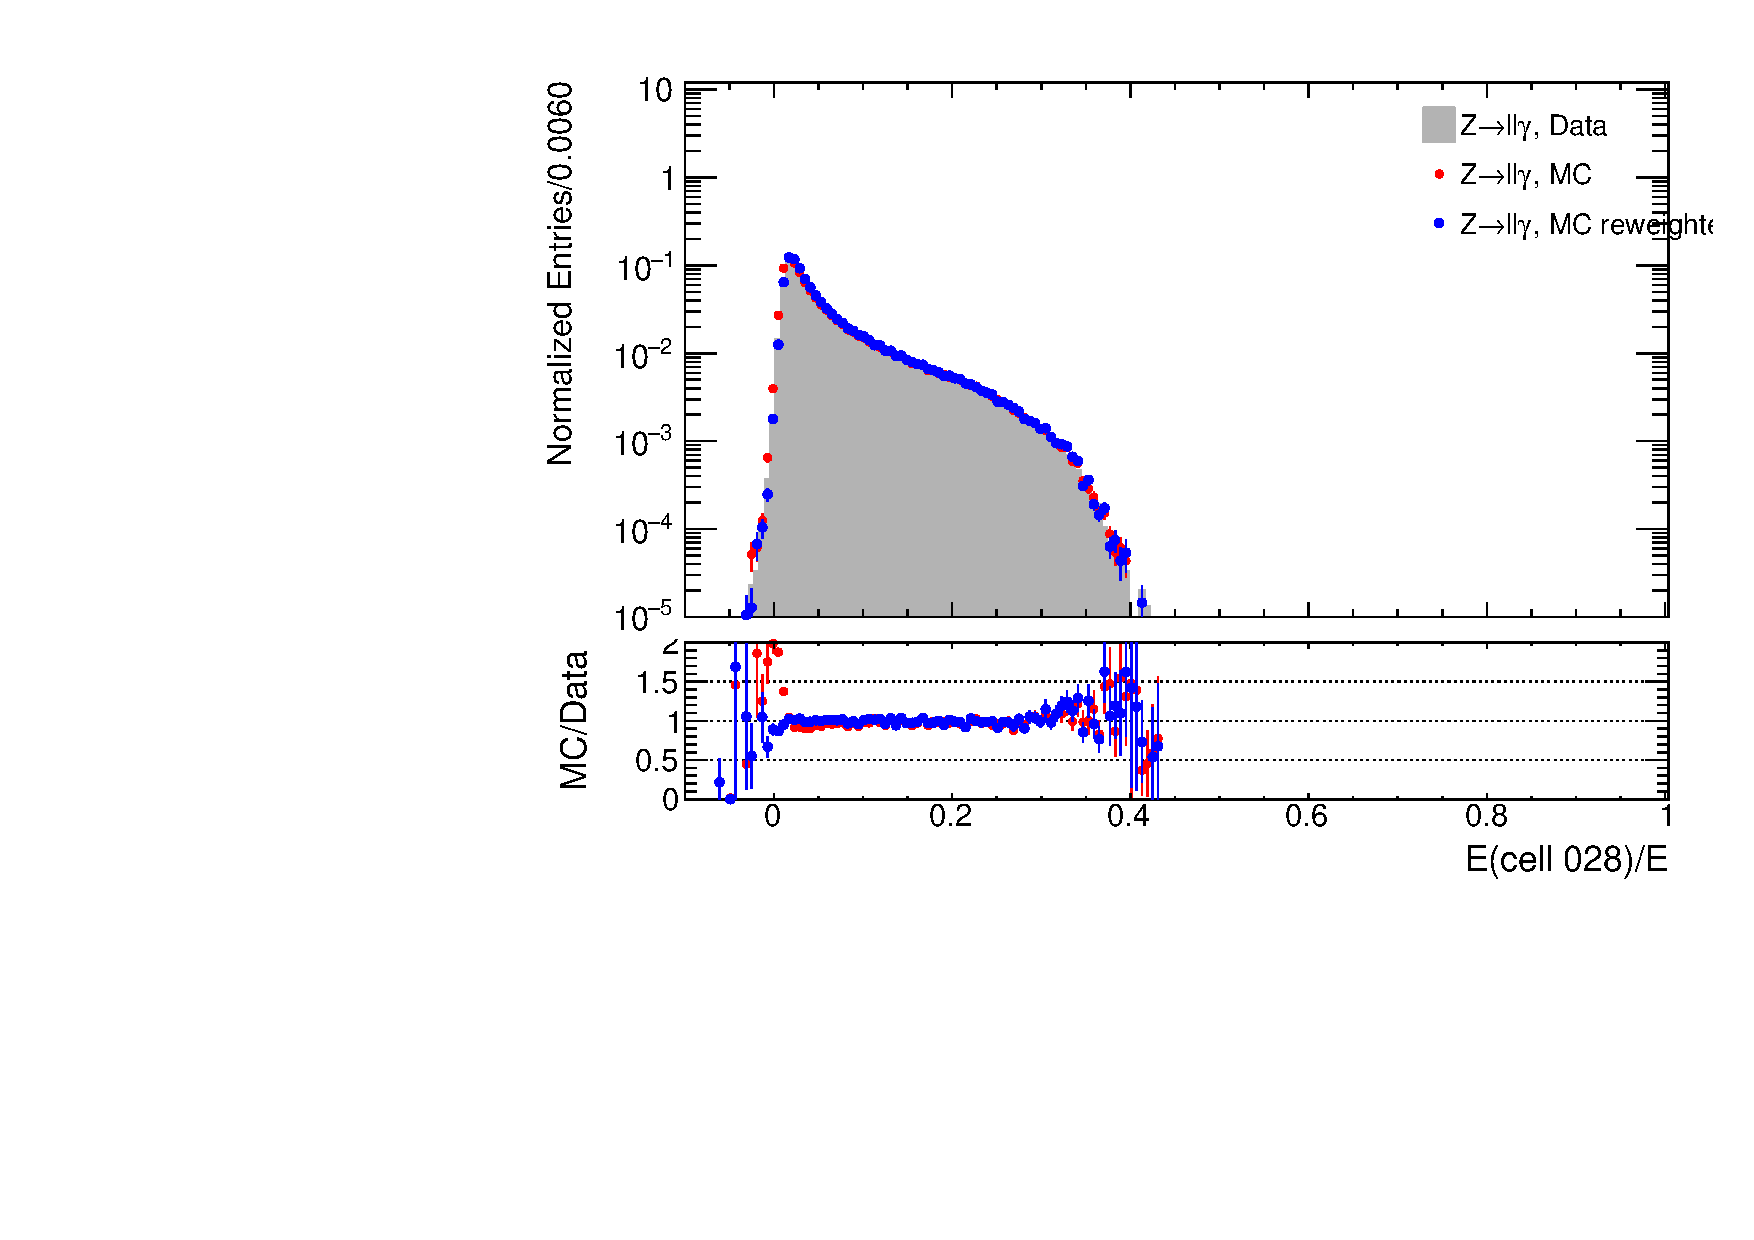
\includegraphics[width=\linewidth]{4_photonid/cell_rw/results/cells/c__u__L2_e_cell_028_normTo1}
        \caption{Celda 28}
    \end{subfigure}
    \hfill
    \begin{subfigure}[h]{0.32\linewidth}
        \centering
        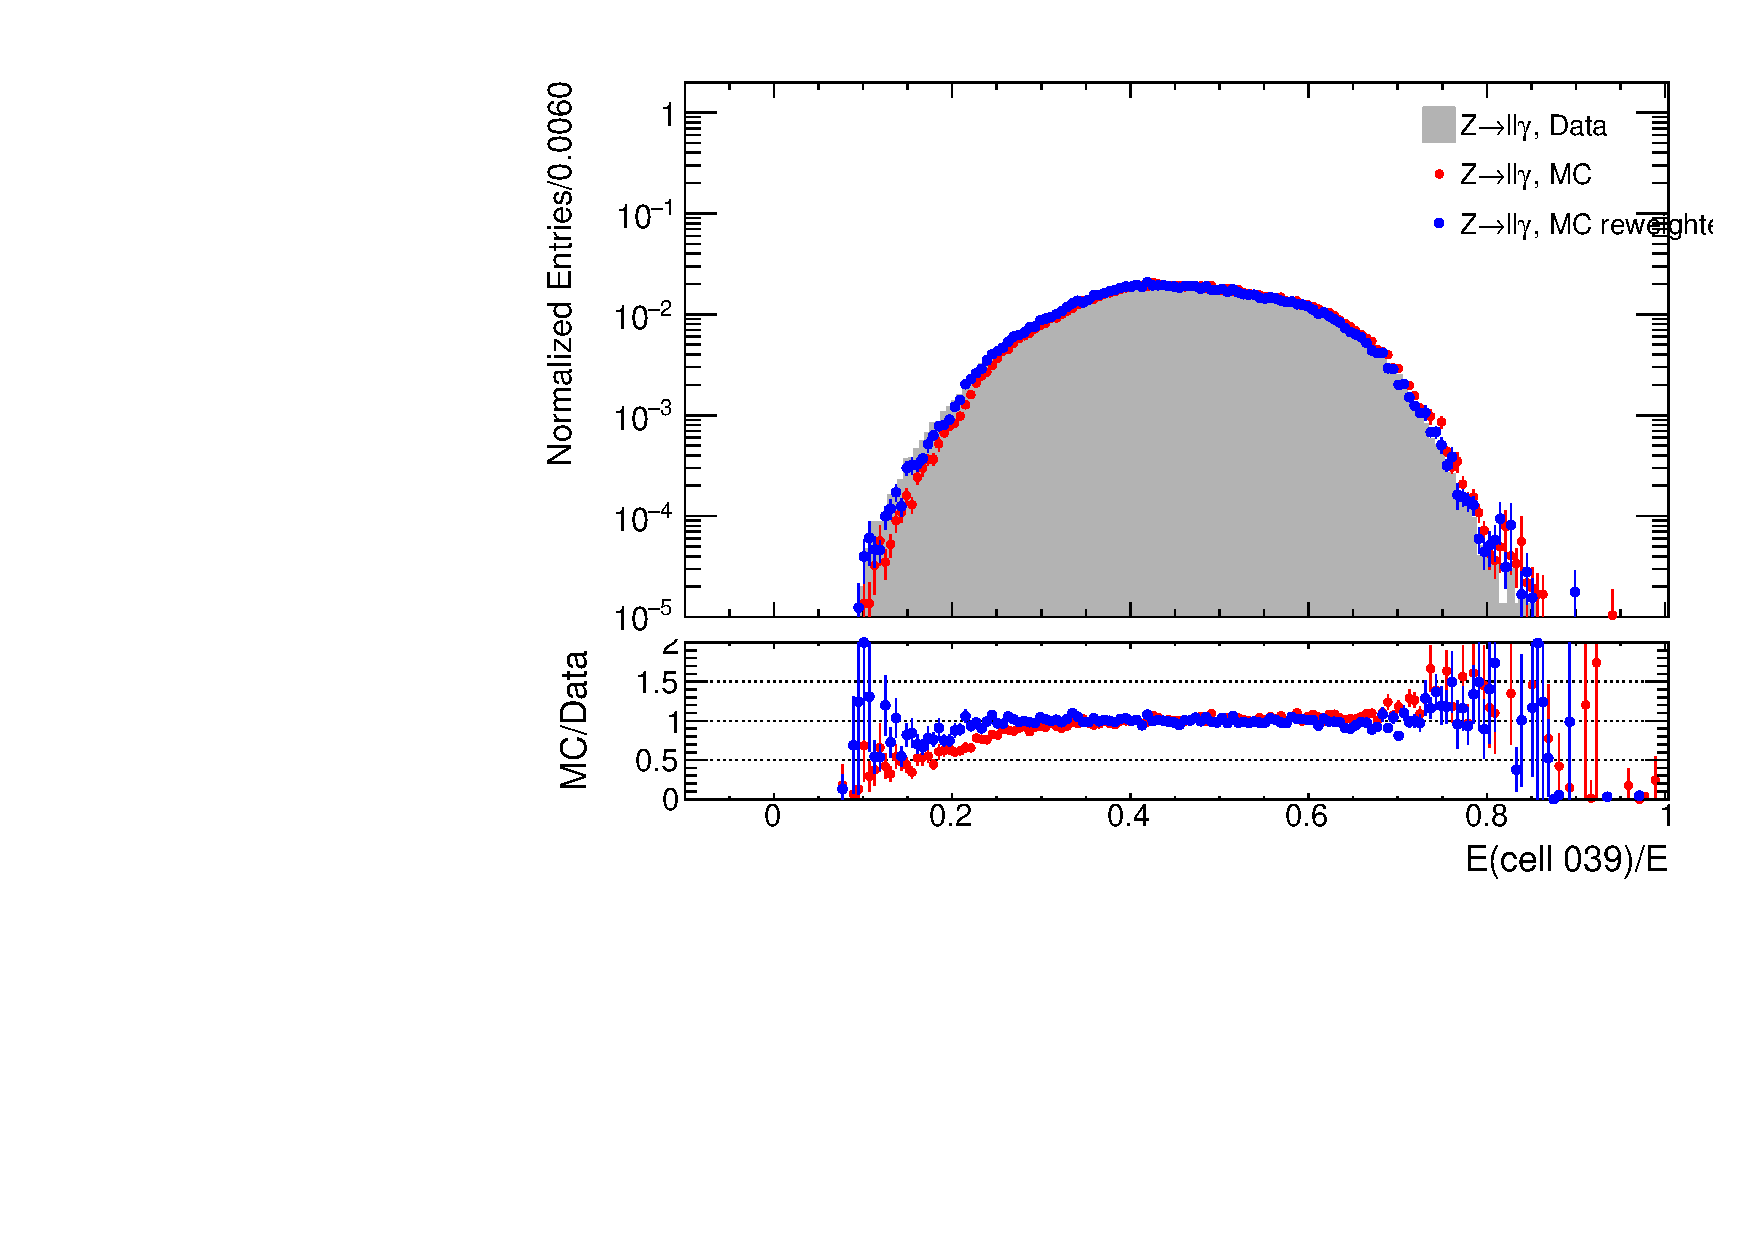
\includegraphics[width=\linewidth]{4_photonid/cell_rw/results/cells/c__u__L2_e_cell_039_normTo1}
        \caption{Celda 39}
    \end{subfigure}
    \hfill
    \begin{subfigure}[h]{0.32\linewidth}
        \centering
        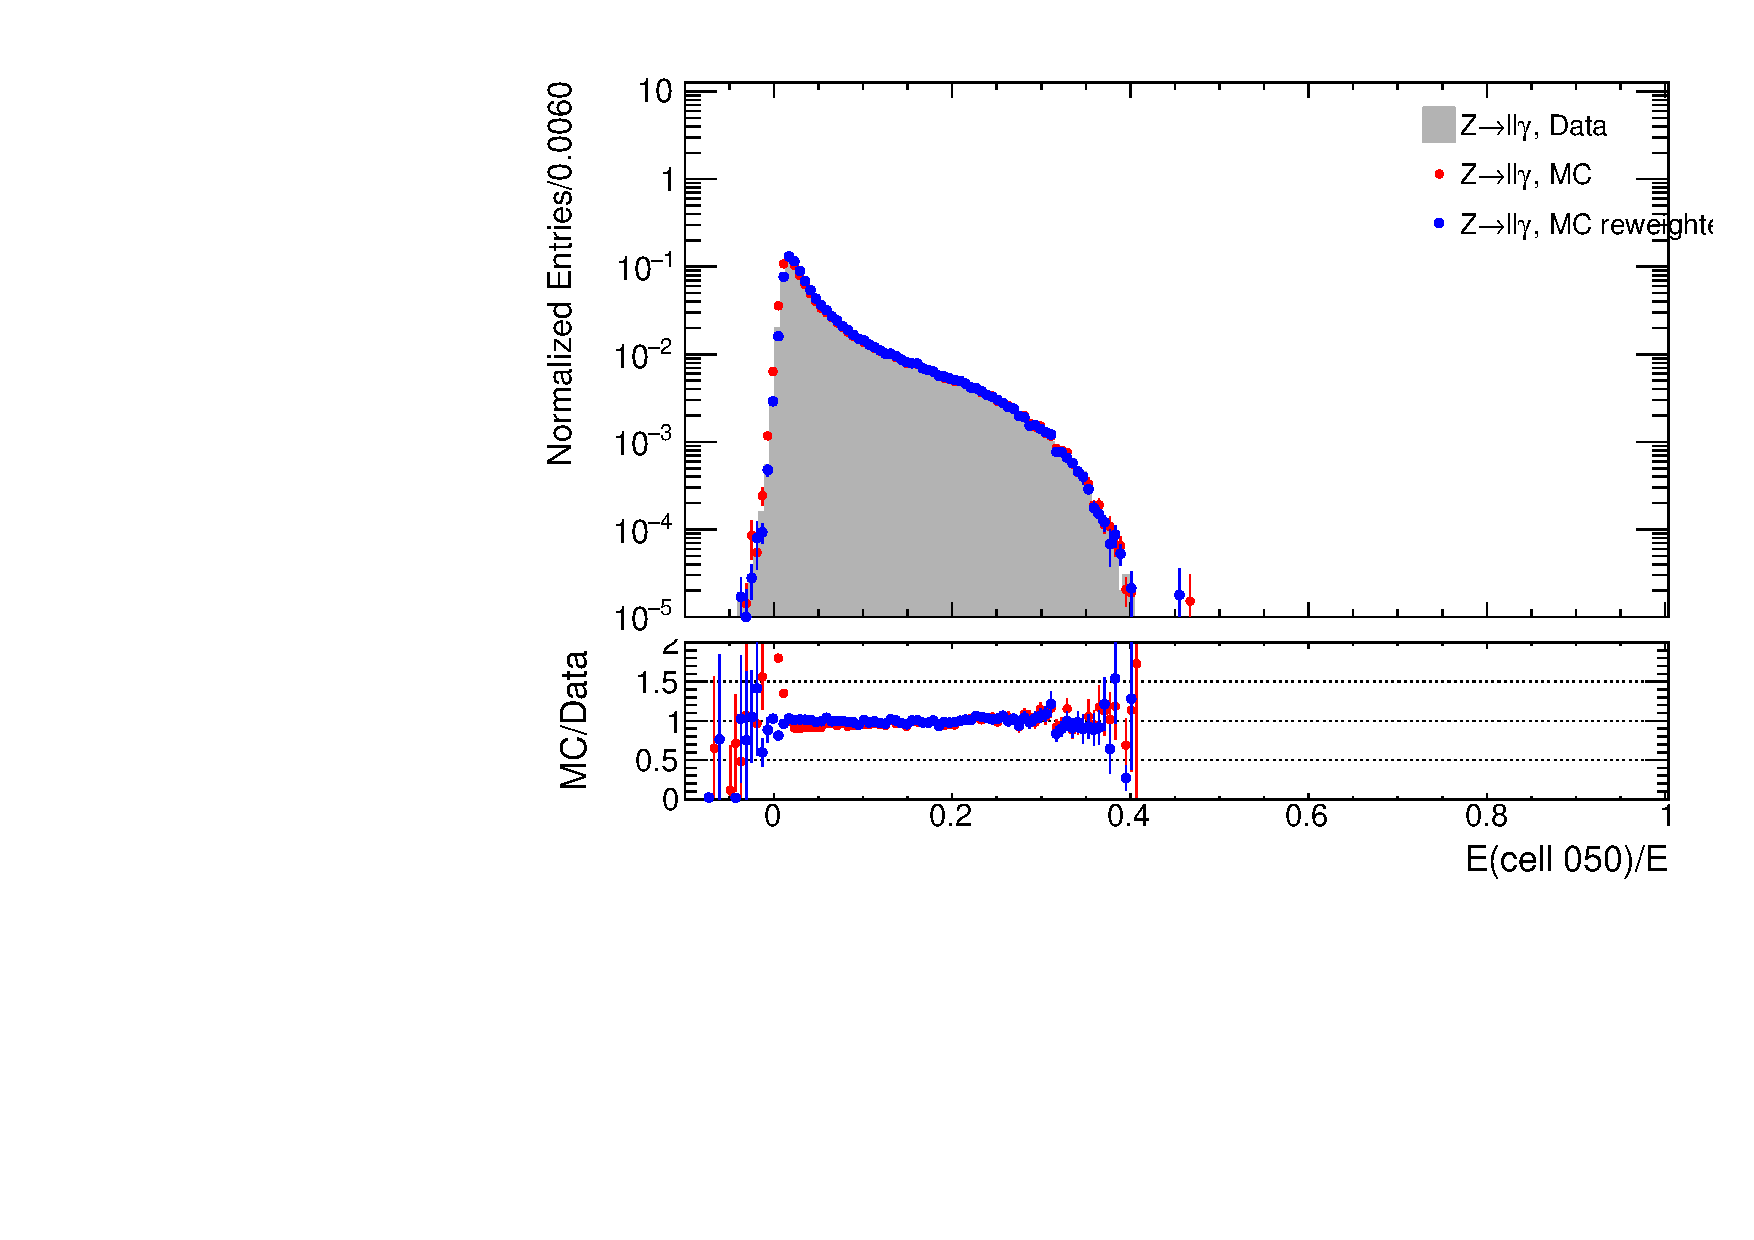
\includegraphics[width=\linewidth]{4_photonid/cell_rw/results/cells/c__u__L2_e_cell_050_normTo1}
        \caption{Celda 50}
    \end{subfigure}
    \caption{Distribuciones de las energías normalizadas de las celdas 28, 39 y 50 de cluster de 77 celdas, para fotones no convertidos. Los puntos azules y rojos corresponden a las distribuciones de la simulación \ac{MC} con y sin las correcciones, respectivamente, mientras que el histograma gris representa los datos.}
    \label{fig:ss_corrections:cell_rw:results:cells}
\end{figure}



Para evaluar el comportamiento del nuevo procedimiento de corrección aplicado a las \acp{SS} de la segunda capa \ac{ECAL}, en la \Fig{\ref{fig:ss_corrections:cell_rw:results:ss}} se muestra la comparación de los métodos de corrección para las variables \reta, \rphi y \weta. En los tres casos se observa una mejora con respecto al \ac{MC} sin corregir especialmente para \rphi y \weta. El método de corrección de energía, en el caso de fotones no convertidos, no alcanza el nivel de acuerdo con los datos logrado por el método de \acp{FF} que ha demostrado proporcionar una excelente acuerdo con los datos experimentales. Sin embargo, casi no se observan diferencias entre el método de corrección de energías y el de \acp{FF} para fotones convertidos lo que indica que aún hay margen de mejora en las correcciones.


\begin{figure}[ht!]
    \centering
    \begin{subfigure}[h]{0.32\linewidth}
        \centering
        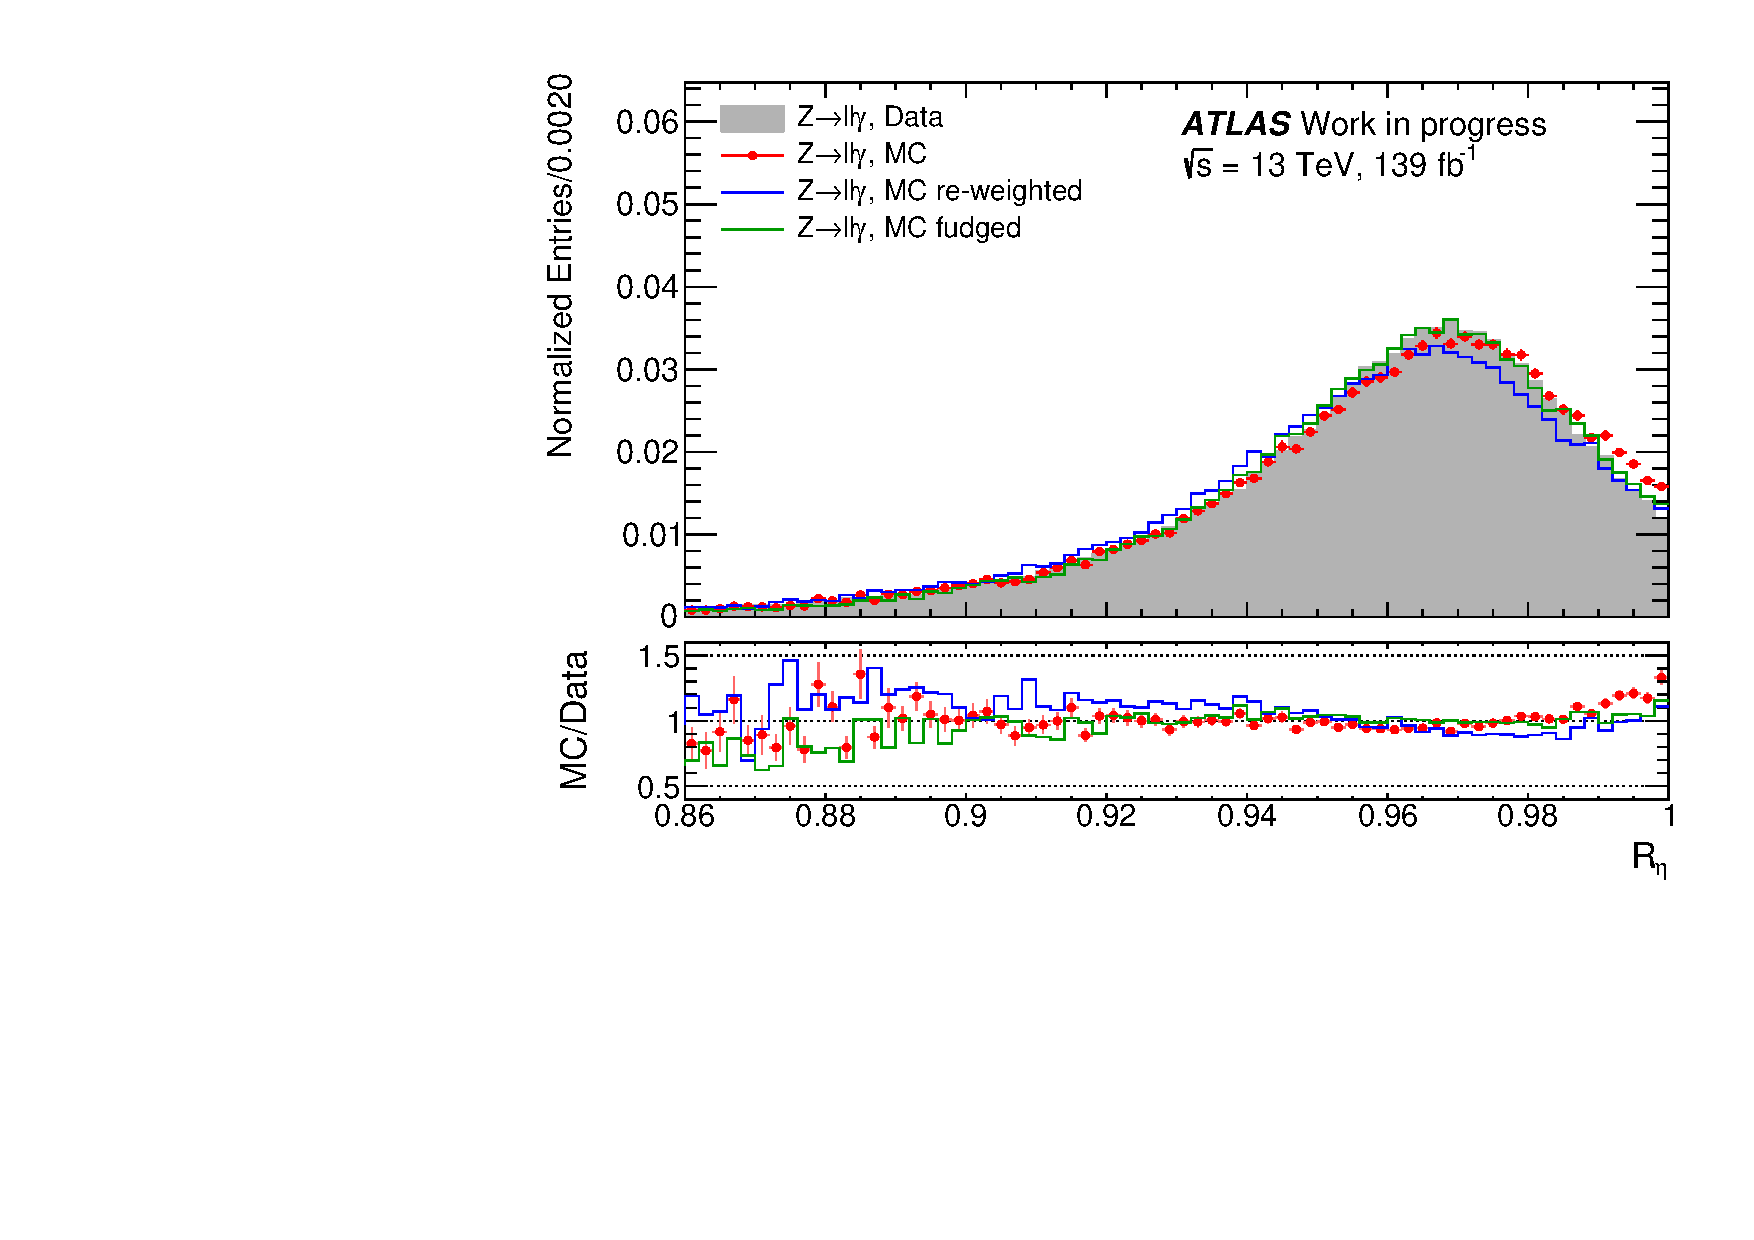
\includegraphics[width=\linewidth]{4_photonid/cell_rw/results/ss/c__u_eta00__ss_Reta}
        \caption{\reta, fotones no convertidos}
    \end{subfigure}
    \hfill
    \begin{subfigure}[h]{0.32\linewidth}
        \centering
        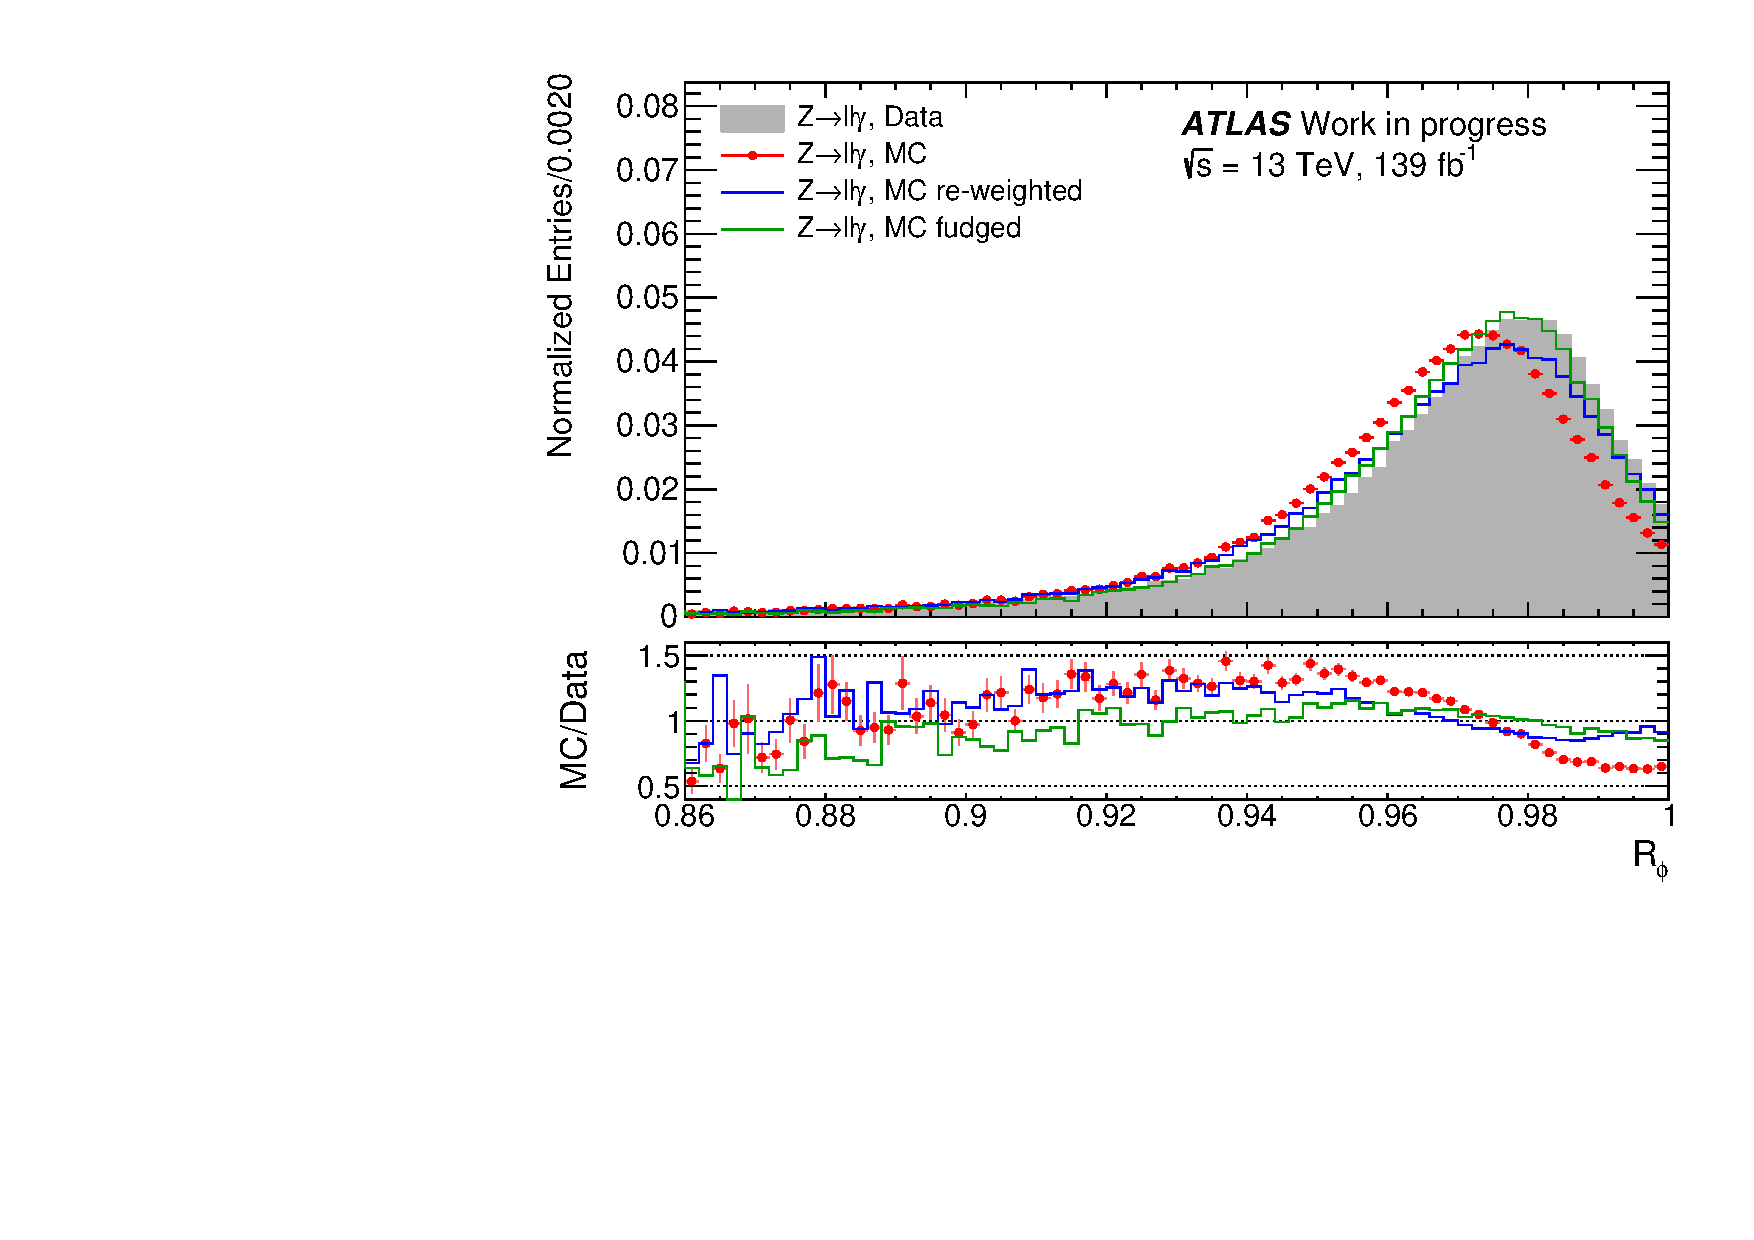
\includegraphics[width=\linewidth]{4_photonid/cell_rw/results/ss/c__u_eta00__ss_Rphi}
        \caption{\rphi, fotones no convertidos}
    \end{subfigure}
    \begin{subfigure}[h]{0.32\linewidth}
        \centering
        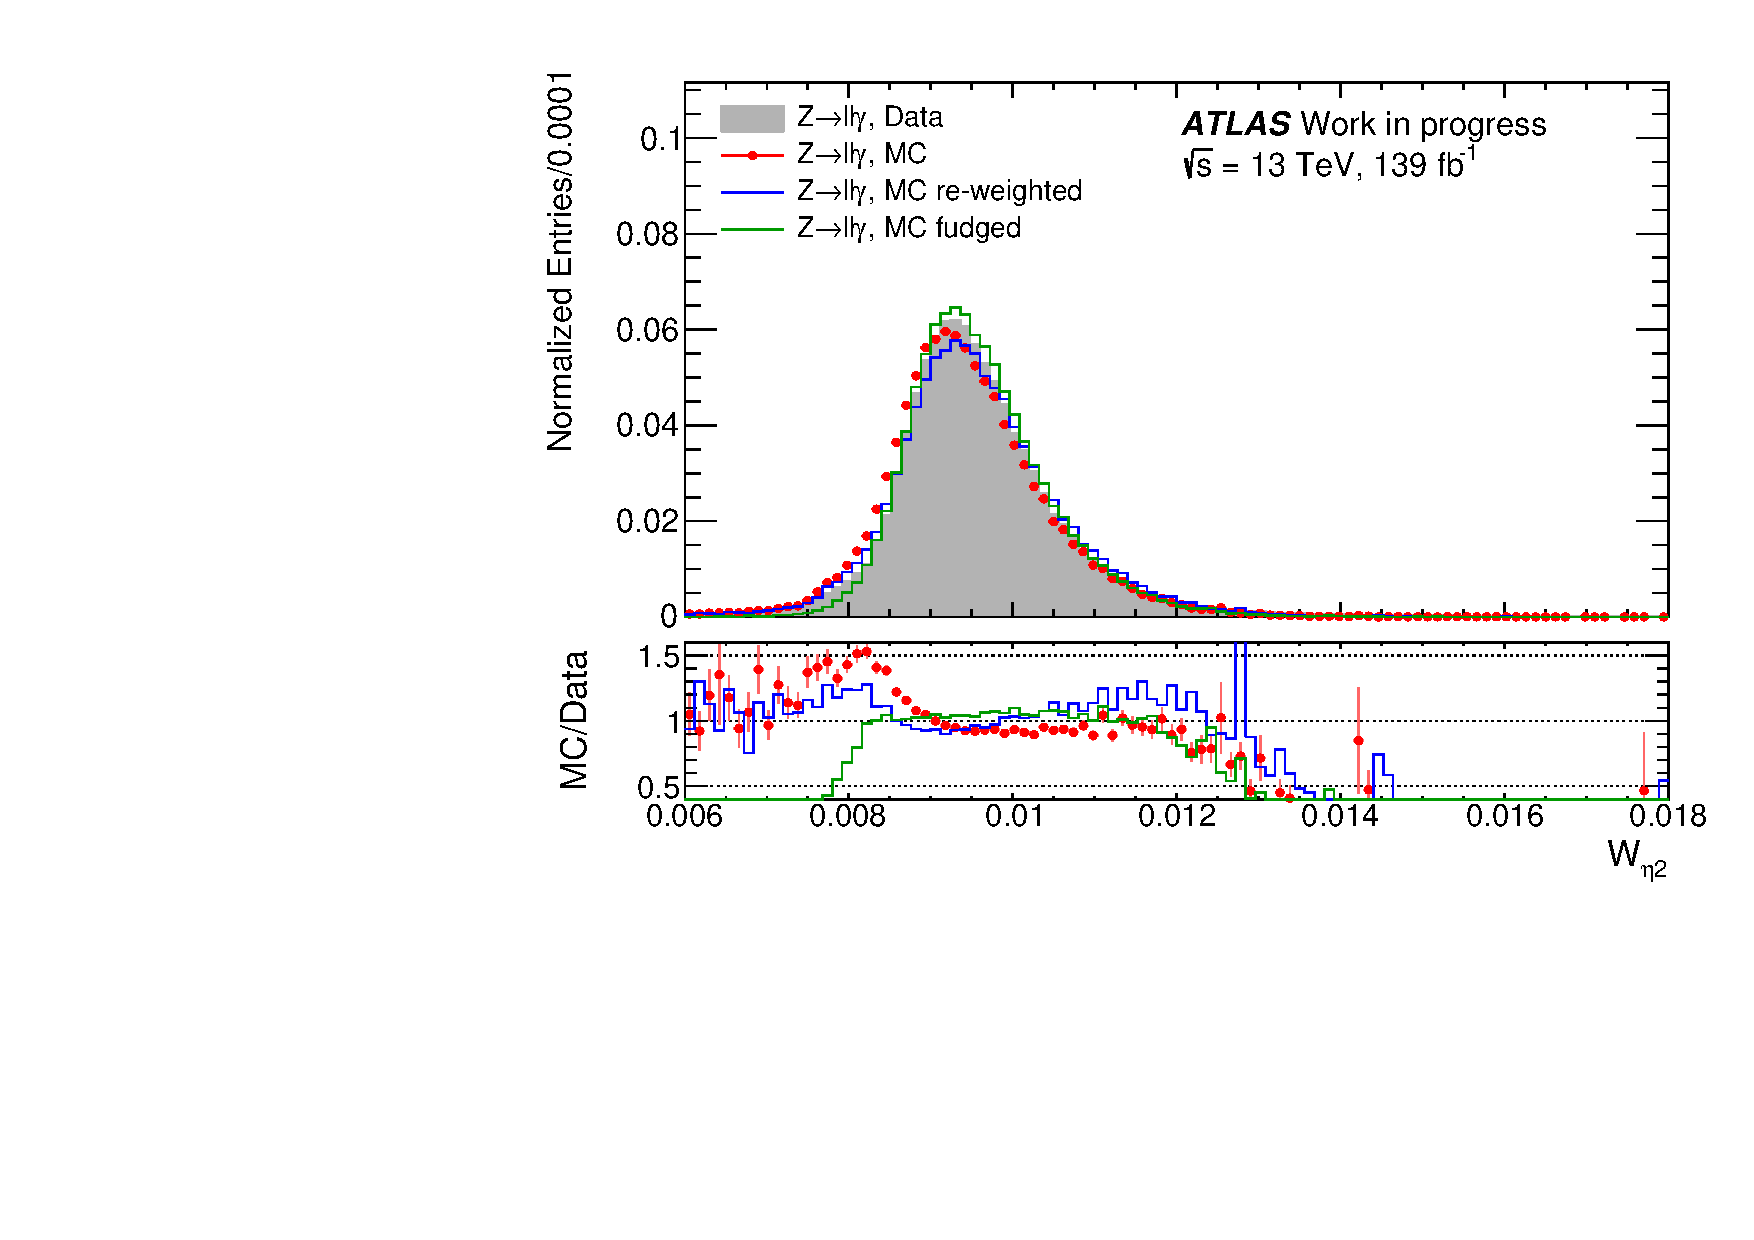
\includegraphics[width=\linewidth]{4_photonid/cell_rw/results/ss/c__u_eta00__ss_Weta2}
        \caption{\weta, fotones no convertidos}
    \end{subfigure}\\
    \begin{subfigure}[h]{0.32\linewidth}
        \centering
        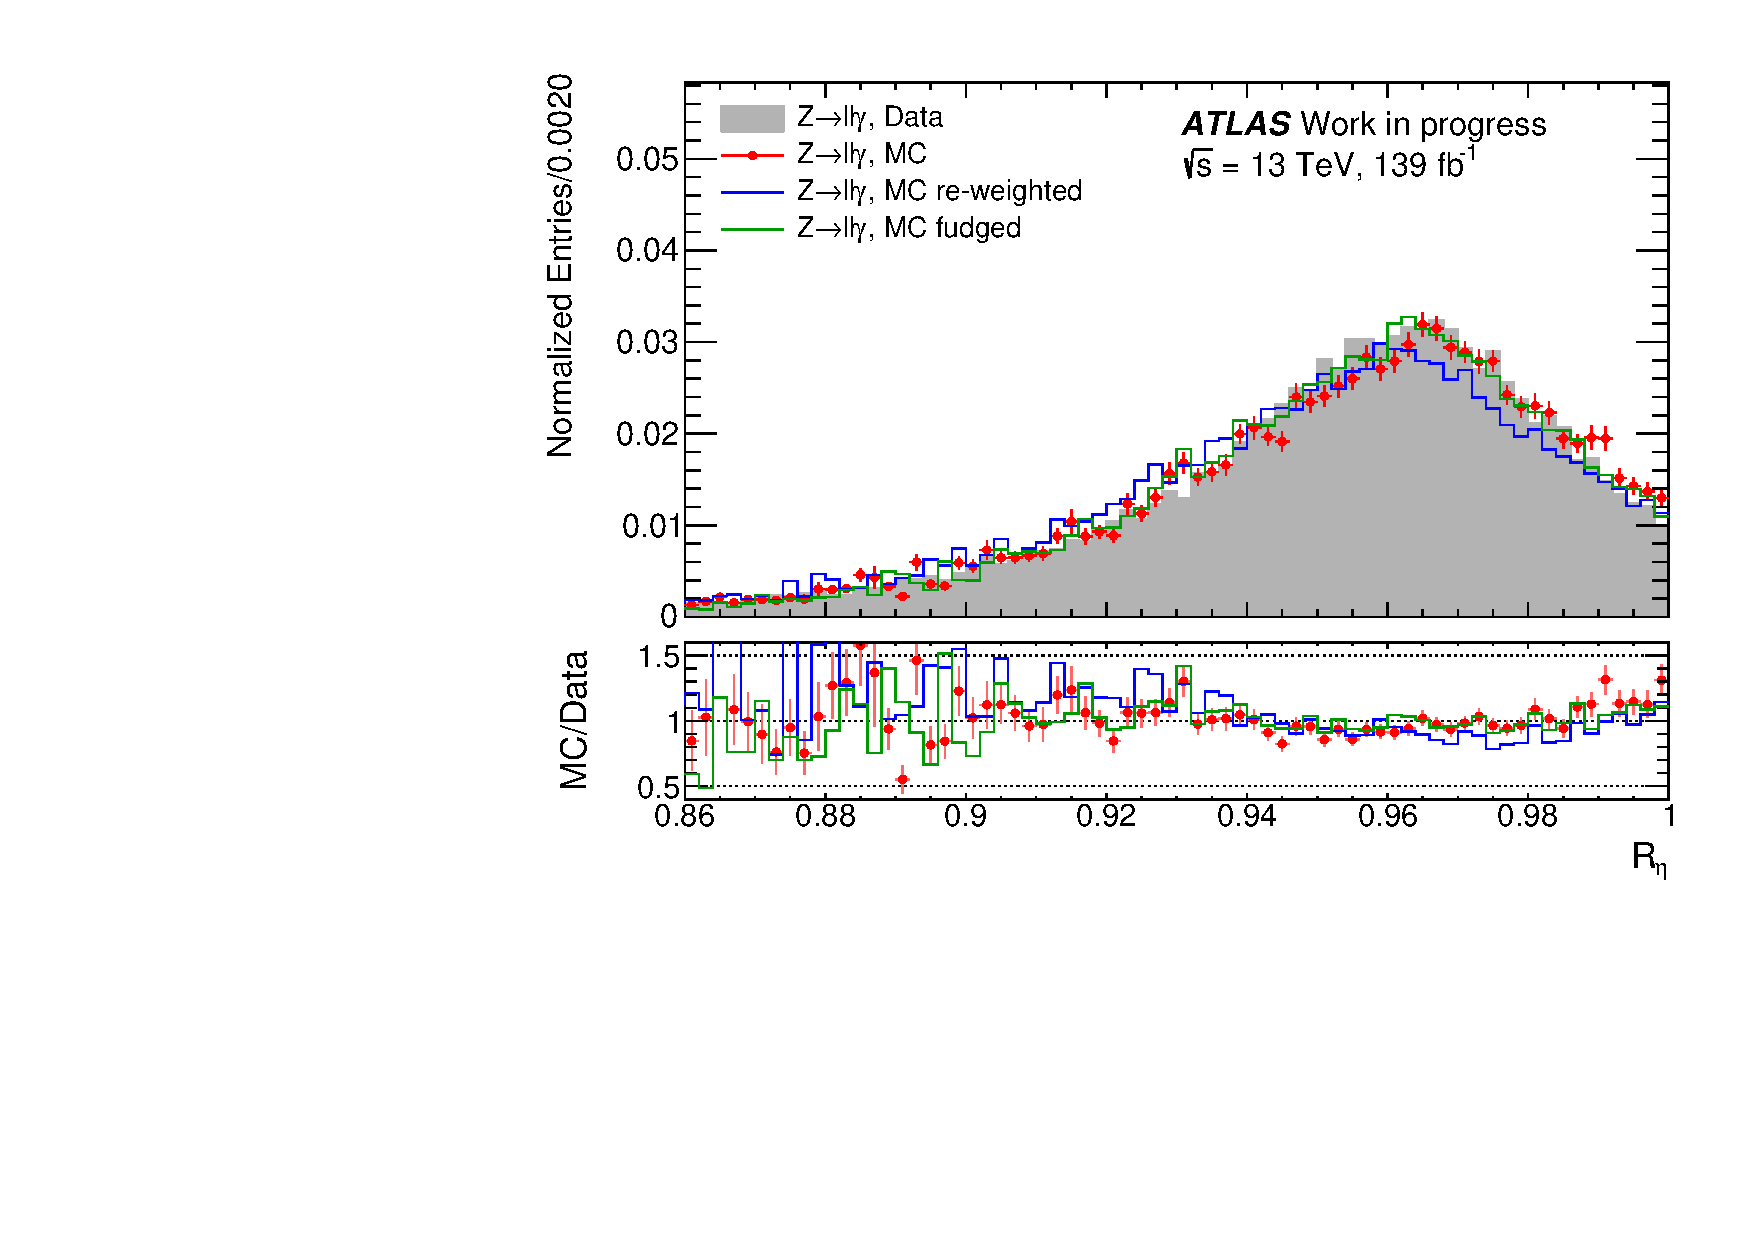
\includegraphics[width=\linewidth]{4_photonid/cell_rw/results/ss/c__c_eta00__ss_Reta}
        \caption{\reta, fotones convertidos}
    \end{subfigure}
    \hfill
    \begin{subfigure}[h]{0.32\linewidth}
        \centering
        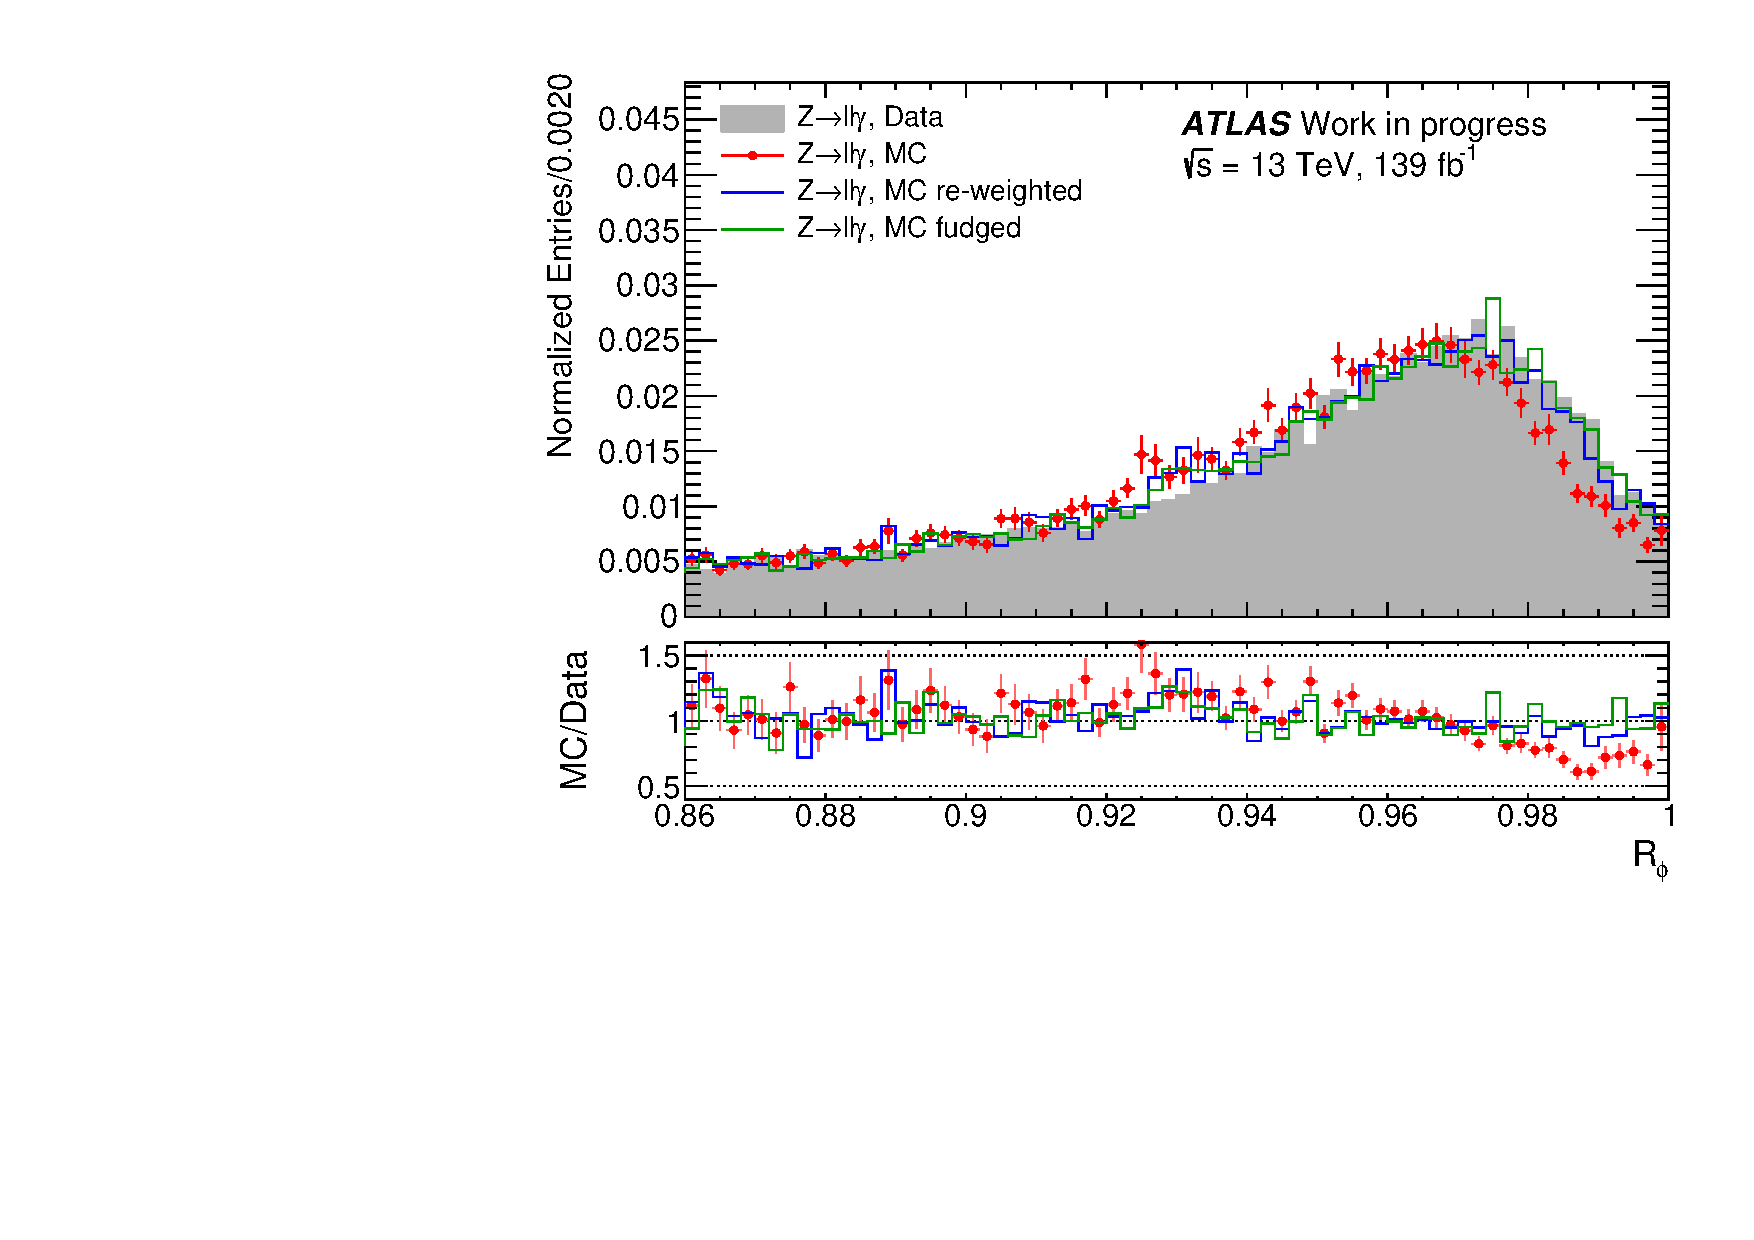
\includegraphics[width=\linewidth]{4_photonid/cell_rw/results/ss/c__c_eta00__ss_Rphi}
        \caption{\rphi, fotones convertidos}
    \end{subfigure}
    \begin{subfigure}[h]{0.32\linewidth}
        \centering
        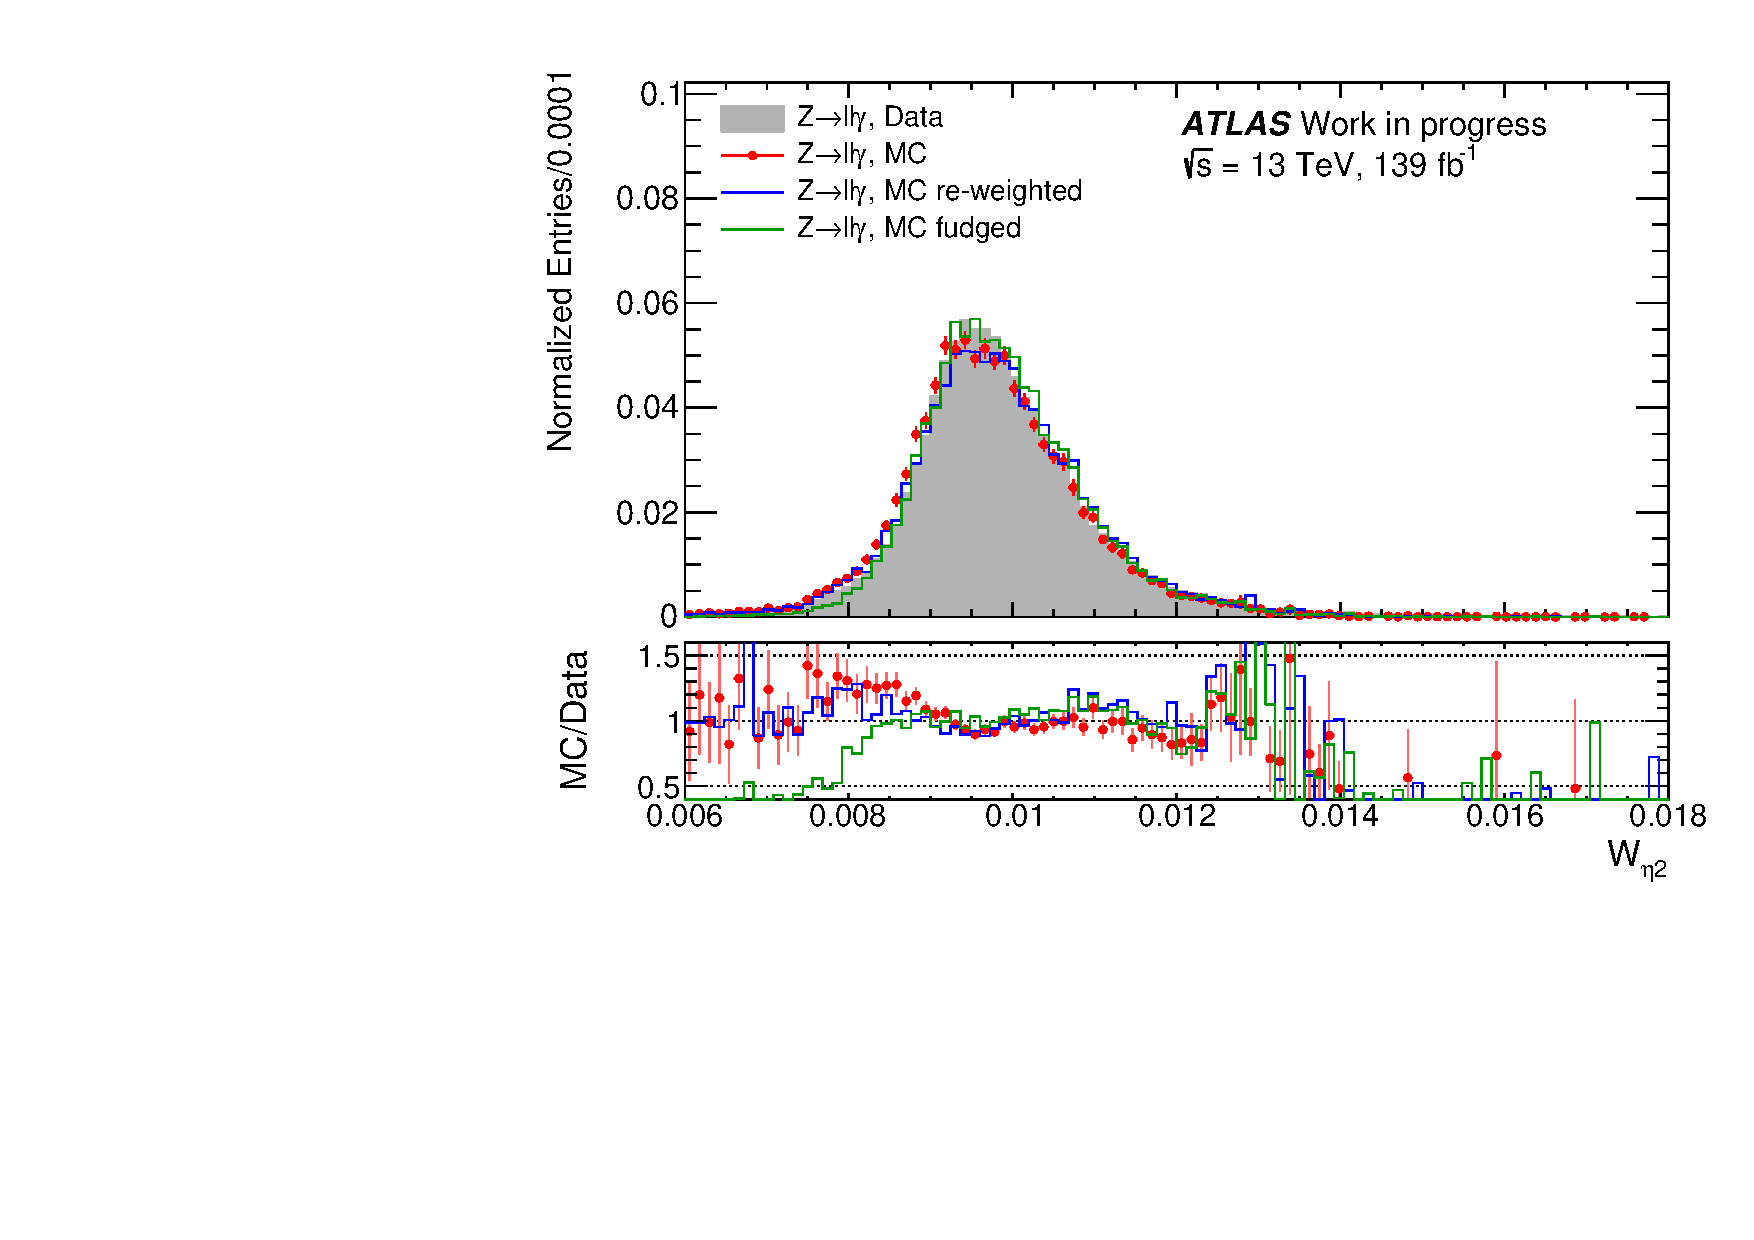
\includegraphics[width=\linewidth]{4_photonid/cell_rw/results/ss/c__c_eta00__ss_Weta2}
        \caption{\weta, fotones convertidos}
    \end{subfigure}\\
    \caption{Distribuciones de las \acp{SS} calculadas en la segunda capa del \ac{ECAL} para fotones no convertidos (fila superior) y convertidos (fila inferior) con pseudorapidez \(\abseta<0.6\), comparando los diferentes métodos de corrección con los datos. Los datos experimentales están representados por los histogramas grises. La simulación \ac{MC} sin corregir se muestra con los puntos rojos, la simulación corregida por el método de corrección de energías con la línea azul y la corregida por el método de \acp{FF} con la línea verde.}
    \label{fig:ss_corrections:cell_rw:results:ss}
\end{figure}






\section{Conclusiones y trabajo futuro}
\label{sec:ss_corrections:summary}

En el presente capítulo se han investigado dos métodos para corregir el desacuerdo observado en las \acfp{SS} entre los datos y la simulación \ac{MC}.

El método de \acf{FF} se ha utilizado históricamente en la colaboración, al principio basado únicamente en simples desplazamientos de las distribuciones. A pesar de que las correcciones conducían a buenas mejoras y, por tanto, a la obtención de mejores \acp{SF}, seguían existiendo notables diferencias de forma entre los datos y la simulación. En el contexto de este trabajo de tesis, al añadir un término lineal a la transformación de la variable se logra corregir los anchos de las distribuciones simuladas, lo que conduce a un acuerdo aún mejor con los datos. Este nuevo método de corrección de \acp{SS} mediante \acp{FF} se denomina método shift+stretch y actualmente se utiliza por toda la colaboración \ac{ATLAS}.

También se ha desarrollado un método de corrección novedoso y que actúa a más bajo nivel, que pretende modificar las energías en las celdas del \ac{ECAL}. Utilizando las distribuciones de energía en cada celda en clusters alrededor de la celda más energética (es decir, utilizando la información de más bajo nivel en el proceso de reconstrucción), es posible corregir todas las \acp{SS} (variables de alto nivel en el proceso de reconstrucción) en simultáneo. Este método usa la misma estrategia de shift+stretch pero esta vez aplicado a las distribuciones de energía normalizada en cada celda de la simulación \ac{MC} para que coincida con la distribución encontrada en los datos. Aunque el método es nuevo y aún necesita de mejoras, como también extenderlo a las demás capas del \ac{ECAL}, ha dado resultados prometedores en los que algunas variables se corrigen de la misma manera que con el \acp{FF}

El método de corrección de las energías de las celdas muestra un gran potencial en la colaboración. Este enfoque podría emplearse en diferentes pasos del proceso de identificación de fotones, como en el nivel de trigger, o de forma \textit{offline} para corregir todos los \acp{SS} simultáneamente. Otro uso potencial e importante es utilizar los clusters corregidos para la identificación de fotones, por ejemplo considerando a los clusters como imágenes y utilizando una red neuronal convolucional (CNN) para realizar la identificación de fotones~\cite{thesis_belfkir}.

Las \acp{SS} tienen la gran ventaja de que se pueden interpretar fácilmente en términos físicos. Por esta razón, mantener estas variables sirve para comprender la física subyacente de los procesos. Seguir corrigiendo estas variables es de gran interés y hay varias formas de hacerlo. El método actual de transformar la variable pero utilizando términos de orden superior sigue siendo una tarea difícil, pero aún no explorada. Haciendo uso de las novedosas técnicas de Machine Learning (ML), es posible obtener factores de corrección para los términos de orden superior en la expansión, corrigiendo además los momentos de orden superior de las distribuciones (asimetría estadística, curtosis, etc.). Otro enfoque interesante es el uso de un re-escaleo multivariable, que se exploró en la \Refn{\cite{thesis_spah}}, mostrando resultados muy prometedores.